\documentclass[11pt,a4paper]{article}
% ------------------------------------------------------------------ packages
\usepackage[T1]{fontenc}
\usepackage{lmodern}
\usepackage[margin=1.1in]{geometry}
\usepackage{amsmath,amssymb,amsthm,mathtools}
\usepackage{microtype}
\usepackage{enumitem}
\usepackage{array,booktabs,tabularx}
\usepackage{xcolor}
\usepackage{tikz}
\usetikzlibrary{arrows.meta,positioning,calc,fit,backgrounds,shapes.geometric,patterns,decorations.pathreplacing}
\usepackage[most]{tcolorbox}
\usepackage[font=small,labelfont=bf,skip=4pt]{caption}
\usepackage[colorlinks=true,linkcolor=blue!50!black,citecolor=teal!55!black,
            urlcolor=violet!65!black,bookmarksnumbered=true]{hyperref}
\usepackage{cleveref}

% ------------------------------------------------------------------ colours
\definecolor{ideacol}{RGB}{255,247,224}
\definecolor{ideaframe}{RGB}{214,178,80}
\definecolor{warncol}{RGB}{253,235,235}
\definecolor{warnframe}{RGB}{200,90,90}
\definecolor{checkcol}{RGB}{235,243,252}
\definecolor{checkframe}{RGB}{90,130,190}
\definecolor{plancol}{RGB}{240,247,240}
\definecolor{planframe}{RGB}{90,150,100}
\definecolor{contractcol}{RGB}{246,242,250}
\definecolor{contractframe}{RGB}{130,100,170}
\definecolor{graytext}{RGB}{90,90,90}

% ------------------------------------------------------------------ theorems
% thmtools is used so that cleveref prints the right environment name even
% though all statement types share one counter (and therefore one numbering).
\usepackage{thmtools}
\declaretheorem[name=Theorem,numberwithin=section,style=definition,
  refname={Theorem,Theorems},Refname={Theorem,Theorems}]{theorem}
\declaretheorem[name=Proposition,numberlike=theorem,style=definition,
  refname={Proposition,Propositions},Refname={Proposition,Propositions}]{proposition}
\declaretheorem[name=Lemma,numberlike=theorem,style=definition,
  refname={Lemma,Lemmas},Refname={Lemma,Lemmas}]{lemma}
\declaretheorem[name=Corollary,numberlike=theorem,style=definition,
  refname={Corollary,Corollaries},Refname={Corollary,Corollaries}]{corollary}
\declaretheorem[name=Definition,numberlike=theorem,style=definition,
  refname={Definition,Definitions},Refname={Definition,Definitions}]{definition}
\declaretheorem[name=Example,numberlike=theorem,style=definition,
  refname={Example,Examples},Refname={Example,Examples}]{example}
\declaretheorem[name=Construction,numberlike=theorem,style=definition,
  refname={Construction,Constructions},Refname={Construction,Constructions}]{construction}
\declaretheorem[name=Remark,numberlike=theorem,style=remark,
  refname={Remark,Remarks},Refname={Remark,Remarks}]{remark}

\crefname{figure}{Figure}{Figures}
\crefname{table}{Table}{Tables}
\crefname{section}{Section}{Sections}
\crefname{appendix}{Appendix}{Appendices}

\numberwithin{equation}{section}

% ------------------------------------------------------------------ boxes
% "In words" gloss, attached above a formal statement
\newtcolorbox{words}{
  enhanced, breakable=false, colback=black!4, colframe=black!4, boxrule=0pt,
  leftrule=2.4pt, arc=0pt, outer arc=0pt, left=7pt, right=7pt, top=3pt, bottom=3pt,
  fontupper=\small\itshape}

% section contract
\newtcolorbox{contract}[1][]{
  enhanced, breakable=true, colback=contractcol, colframe=contractframe,
  boxrule=0.6pt, arc=2pt, left=7pt, right=7pt, top=13pt, bottom=5pt,
  fonttitle=\small\bfseries\sffamily, title={What this section does},
  attach boxed title to top left={xshift=8pt, yshift=-8pt},
  boxed title style={colback=contractframe, colframe=contractframe, arc=1pt},
  #1}

% proof plan
\newtcolorbox{planbox}[1][Proof plan]{
  enhanced, breakable=true, colback=plancol, colframe=planframe,
  boxrule=0.5pt, arc=2pt, left=7pt, right=7pt, top=12pt, bottom=4pt,
  fonttitle=\small\bfseries, title={#1},
  attach boxed title to top left={xshift=6pt, yshift=-7pt},
  boxed title style={colback=planframe, colframe=planframe, arc=1pt, left=3pt,right=3pt,top=1pt,bottom=1pt}}

% idea / warning / checkpoint
\newtcolorbox{ideabox}[1][]{
  enhanced, breakable=true, colback=ideacol, colframe=ideaframe, boxrule=0.6pt,
  arc=2pt, left=7pt, right=7pt, top=12pt, bottom=4pt,
  fonttitle=\small\bfseries, title={Idea},
  attach boxed title to top left={xshift=6pt, yshift=-7pt},
  boxed title style={colback=ideaframe, colframe=ideaframe, arc=1pt, left=3pt,right=3pt,top=1pt,bottom=1pt},
  #1}
\newtcolorbox{warnbox}[1][]{
  enhanced, breakable=true, colback=warncol, colframe=warnframe, boxrule=0.6pt,
  arc=2pt, left=7pt, right=7pt, top=12pt, bottom=4pt,
  fonttitle=\small\bfseries, title={Watch out},
  attach boxed title to top left={xshift=6pt, yshift=-7pt},
  boxed title style={colback=warnframe, colframe=warnframe, arc=1pt, left=3pt,right=3pt,top=1pt,bottom=1pt},
  #1}
\newtcolorbox{checkpoint}[1][]{
  enhanced, breakable=true, colback=checkcol, colframe=checkframe, boxrule=0.6pt,
  arc=2pt, left=7pt, right=7pt, top=12pt, bottom=4pt,
  fonttitle=\small\bfseries, title={Where we are},
  attach boxed title to top left={xshift=6pt, yshift=-7pt},
  boxed title style={colback=checkframe, colframe=checkframe, arc=1pt, left=3pt,right=3pt,top=1pt,bottom=1pt},
  #1}

% "used in" line
\newcommand{\usedin}[1]{\par\smallskip\noindent{\small\color{graytext}\textbf{Used in:} #1.}}

% ------------------------------------------------------------------ macros
\newcommand{\abs}[1]{\lvert #1\rvert}
\newcommand{\card}[1]{\lvert #1\rvert}
\DeclareMathOperator{\rank}{rank}
\DeclareMathOperator{\im}{im}
\DeclareMathOperator{\Span}{span}
\newcommand{\R}{\mathbb R}
\newcommand{\from}{\leftarrow}
\newcommand{\disjoint}{\sqcup}
\newcommand{\Ne}{N_1^+}
\newcommand{\Nee}{N_2^+}
\newcommand{\Nminus}{N_1^-}
\newcommand{\restr}{\upharpoonright}
\DeclareMathOperator{\dom}{dom}
\DeclareMathOperator{\coker}{coker}
\newcommand{\Emph}[1]{\emph{#1}}
\newcommand{\code}[1]{\texttt{#1}}

% theorem-attached "In words" convenience
\newcommand{\inwords}[1]{\begin{words}#1\end{words}}

% step heading inside proofs
\newcommand{\steplabel}[1]{\par\smallskip\noindent\textbf{#1}\quad}

\hypersetup{pdftitle={A proof of Seymour's second-neighborhood conjecture --- a guided rewrite},
            pdfauthor={after OpenAI}, pdfsubject={Oriented graphs, second neighborhoods}}

\title{\bfseries A proof of Seymour's second-neighborhood conjecture\\[2pt]
\large A guided, figure-rich rewrite}
\author{after the preprint of OpenAI, September 23, 2026\\[2pt]
\small rewritten for readability; the mathematics is unchanged}
\date{}

\begin{document}
\maketitle

\begin{abstract}
\noindent
Every nonempty finite \emph{oriented} graph has a vertex with at least as many vertices at
directed distance exactly two as at directed distance one. This settles Seymour's
second-neighborhood conjecture in full generality.

\smallskip
\noindent
The proof has three moving parts, and this document is organised around them.
\emph{(i) Reduction.} A minimal counterexample yields, for every nonempty proper vertex set
$S$, a strict inequality $\abs{F^2(S)\setminus F(S)}<\abs{F(S)\setminus S}$ between a second
image and a first image; a transitive-tournament blowup converts it into
$\abs{U}+\abs{F^2(U)}<2\abs{F(U)}$ for every nonempty proper $U$.
\emph{(ii) Pruning.} Two families of ordered pairs that are almost compatible can be made
compatible by deleting few members, at a cost charged partly to the points left uncovered.
\emph{(iii) Extremal contradiction.} Maximising $\abs{P}+\abs{Q}$ plus the number of uncovered
points produces, through \emph{(i)} and \emph{(ii)}, a strictly better pair.

\smallskip
\noindent
This is a rewritten presentation of the preprint of OpenAI (23 September 2026). No statement
has been weakened, no case removed, and no proof step dropped; what is added is structure,
pictures, motivation, and an explicit record of how each step was checked. A dictionary in
\appref{app:dictionary} translates the notation back to the original.
\end{abstract}

\tableofcontents
\bigskip

\section*{How to read this paper}
\addcontentsline{toc}{section}{How to read this paper}
\markboth{How to read this paper}{How to read this paper}

The proof is short in outline and long in detail, and the details are of three very different
kinds: bookkeeping about subsets, a linear-algebra argument about matchings, and an extremal
choice. They are much easier to absorb one at a time. So:

\begin{description}[leftmargin=1.2em,itemsep=2pt]
\item[Level 1 --- five minutes.] Read \cref{sec:intro}, look at \cref{fig:roadmap}, and read the
  boxed \emph{Idea} passages. You will know what is proved and what the three engines are.
\item[Level 2 --- an hour.] Read \cref{sec:reduction,sec:incompatibility} (which use each other)
  and skip \cref{sec:pruning} on a first pass, taking \cref{lem:pruning} as a black box. Then read
  \cref{sec:pruning} only for the statement and the shape of the argument. \Cref{sec:weighted,sec:cycles}
  are consequences and are not needed for the main theorem.
\item[Level 3 --- a day.] Everything, in order, including the toolkit (\appref{app:toolkit}), which
  proves the five facts taken from outside graph theory, and the verification appendix
  (\appref{app:checks}), which records how each step was checked.
\end{description}

\paragraph{Conventions.}
\begin{itemize}[leftmargin=1.2em,itemsep=1pt]
\item All graphs are finite, and \emph{oriented} means: no loops, no two arcs between the same
  pair of vertices in the same direction, and never both $x\to y$ and $y\to x$.
\item $F(S)$ is the union of the out-neighborhoods of the vertices of $S$; it \emph{never}
  subtracts $S$. This convention is used constantly and is stated again where it matters.
\item $|S|$ is the cardinality of a finite set, $\setminus$ is set difference, and $\sqcup$ is a
  disjoint union (used when the two parts are known to be disjoint).
\item The word \emph{proper} means $\neq$ the whole vertex set; \emph{nonempty proper} subsets are
  the only subsets that ever appear in the subset inequalities.
\end{itemize}

\paragraph{The four kinds of box.} Each has a fixed job, so you can decide at a glance whether to
read it.
\begin{itemize}[leftmargin=1.2em,itemsep=1pt]
\item A \emph{What this section does} box opens every section: assumptions in, result out, and why
  the section exists.
\item An \emph{Idea} box says why a definition or a strategy is the right one. It is motivation,
  not part of any proof.
\item A \emph{Watch out} box flags a trap: a hypothesis that is silently used, or a plausible
  statement that is false.
\item A \emph{Where we are} box appears at the junctions of the long argument and says what has
  been established so far.
\end{itemize}
Formal statements are preceded by a grey \emph{In words} line: one sentence without symbols
saying what the statement asserts, so that you can read the statement without parsing it. Long
proofs are preceded by a green \emph{Proof plan} and split into labeled steps.

\paragraph{Notation at a glance.} Every symbol used in the paper appears here, once, with the
place where it is introduced. The dictionary in \appref{app:dictionary} translates back to the
notation of the original preprint.

{\small
\renewcommand{\arraystretch}{1.16}
\noindent\begin{tabularx}{\textwidth}{@{}lX@{}}
\toprule
\textbf{Symbol} & \textbf{Meaning} \\
\midrule
$G$, $D$, $V(G)$, $A(G)$ & an oriented graph, its vertex set, its arc set; $x\to y$ means $(x,y)\in A(G)$ \\
$n$ & the number of vertices (\emph{order}) of the graph under discussion \\
$F(S)$ & $\{y:\ \exists x\in S,\ x\to y\}$; the union of out-neighborhoods, never subtracting $S$ (\cref{sec:intro}) \\
$F^0(S),F^2(S),F^k(S)$ & $F^0(S)=S$, $F^{k+1}(S)=F(F^k(S))$; $F^2=F\circ F$ \\
$N_1^+(v)$, $N_2^+(v)$ & first and \emph{exact} second out-neighborhood: $F(\{v\})$ and $F^2(\{v\})\setminus F(\{v\})$ \\
$d^+(v)$, $d^-(v)$, $\delta^\pm(D)$ & out-degree, in-degree, and their minima over $V(D)$; $d^\pm$ only in \cref{sec:cycles} \\
$S$, $I$, $E$ & a vertex set, and its split $I=F(S)\cap S$, $E=F(S)\setminus S$ (\cref{sec:reduction}) \\
$g(Y)$ & $\abs{F(Y)\setminus(I\cup Y)}$, the counted quantity in \cref{lem:deficit} \\
$Y$, $D_Y$ & a subset of $E$, and $D$ with all arcs $S\to E\setminus Y$ deleted \\
$Q_v$ & $F(\{v\})\cap(E\setminus Y)$: the out-neighbors of $v$ that the deletion above removes \\
$\Lambda$ & $F(Q_v)\setminus(I\cup Y\cup Q_v\cup F(Y))$: second out-neighbors lost by the deletion \\
$m$, $T_m$, $\tau$, $U$ & block size, transitive tournament on $m$ vertices, its internal image operator, and a vertex set of the blowup (\cref{sec:reduction}) \\
$W$ & $F(S)\cup F^2(S)$: the set of blocks that are completely filled (\cref{lem:blowup}) \\
$X$, $X\times X$ & the vertex set of the graph $G$ of \cref{sec:incompatibility}, and the set of ordered pairs \\
$\Phi_1 P$, $\Phi_2 Q$ & coordinate images of a family of pairs: advance the first, resp.\ second, coordinate along an arc \\
$\Delta$ & $\{(v,v):v\in X\}$, the diagonal \\
$P$, $Q$, $M$ & the extremal left and right families and $M=|P|+|Q|$ \\
$P_j$, $Q_i$ & the column $\{p:(p,j)\in P\}$ and the row $\{s:(i,s)\in Q\}$ \\
$u$, $u'$ & the number of uncovered points, before and after pruning \\
$\mathcal L$, $\mathcal R$ & the left and right family of pairs of \cref{lem:pruning}; in \cref{sec:incompatibility} they are the complements of $\Phi_2^2Q$, $\Phi_1^2P$ \\
$\mathcal L'$, $\mathcal R'$ & the subfamilies retained by the pruning lemma \\
$Z$, $H$ & the conflict points $(i,j)$ and the collision pairs $(p,s)$ of \cref{lem:pruning} \\
$q$ & the number of points of $Z$ left uncovered by $\mathcal L'\cup\mathcal R'$ \\
$\Gamma$, $K$, $\mathcal M$ & the augmented bipartite graph, a vertex cover of it, a maximum matching \\
$k$, $\ell$, $t$ & the numbers of original--original, left--$Z$, and $Z$--right edges of $\mathcal M$ \\
$L$, $N$, $A$, $B$ & the four linear maps of the commuting square \eqref{eq:commute} \\
$D^{p,i}$, $T^{p,i}$ & auxiliary matrix for the pair of indices $p\to i$, and its allowed support \\
$J_p$, $S_i$ & $\{j:(p,j)\in\mathcal L\}$ and $\{s:(i,s)\in\mathcal R\}$ \\
$a_{xy}$, $b_{xy}$ & two independent arrays of variables, one per arc $x\to y$ \\
$\overline N(v)$ & the non-neighbors of $v$: $V\setminus(\{v\}\cup N_1^+(v)\cup N_1^-(v))$ (\cref{sec:cycles}) \\
\bottomrule
\end{tabularx}}

\section{Introduction}\label{sec:intro}

\begin{contract}
\textbf{Assumes:} nothing. \quad
\textbf{Produces:} the statement of the conjecture and of the main theorem
(\cref{thm:main}), the two elementary observations that fix the meaning of the definitions, and a
map of the proof (\cref{fig:roadmap}) naming its three engines.\\[2pt]
\textbf{Why:} the proof is an interplay of three ingredients that are individually simple and
collectively confusing. Knowing which is which before starting is most of the battle.
\end{contract}

\subsection{The conjecture}

An \emph{oriented graph} is a finite directed graph with no loops, no two arcs with the same tail
and head, and no pair of opposite arcs: if $x\to y$ then not $y\to x$. Its underlying undirected
graph need not be complete and need not be connected.

For a vertex $v$,
\begin{equation}\label{eq:N1N2}
 N_1^+(v)=\{u:\ v\to u\},\qquad
 N_2^+(v)=\bigl\{w\notin\{v\}\cup N_1^+(v):\ \text{there is }u\text{ with }v\to u\to w\bigr\}.
\end{equation}
So $N_1^+(v)$ is the set of out-neighbors and $N_2^+(v)$ is the set of vertices at directed
distance \emph{exactly} two. Each vertex is counted once, however many two-step paths reach it.

\begin{figure}[t]
\centering
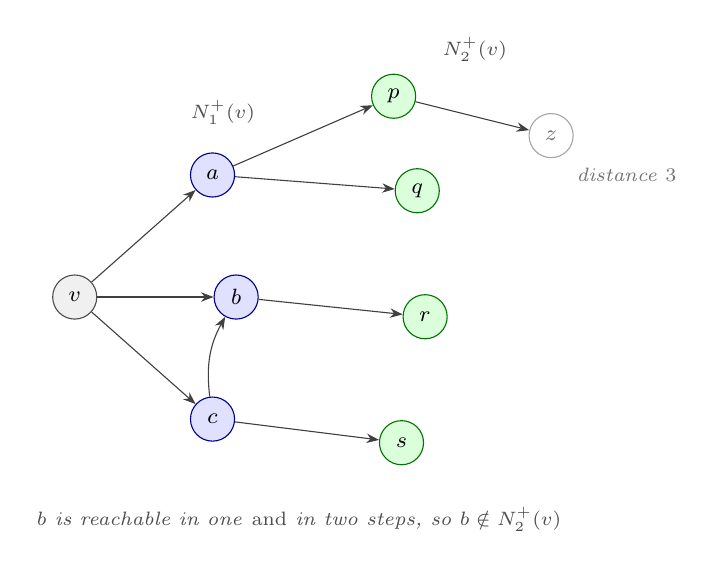
\begin{tikzpicture}[
  vertex/.style={circle,draw=black!70,fill=black!6,inner sep=0pt,minimum size=5.6mm,
                 font=\footnotesize},
  first/.style={circle,draw=blue!55!black,fill=blue!12,inner sep=0pt,minimum size=5.6mm,
                font=\footnotesize},
  second/.style={circle,draw=green!45!black,fill=green!14,inner sep=0pt,minimum size=5.6mm,
                 font=\footnotesize},
  far/.style={circle,draw=black!35,fill=white,inner sep=0pt,minimum size=5.6mm,
              font=\footnotesize,text=black!55},
  arc/.style={-{Stealth[length=1.6mm]},draw=black!75},
  lab/.style={font=\scriptsize\itshape,text=black!70}
]
% vertices
\node[vertex] (v) at (0,0) {$v$};
\node[first]  (a) at (1.75,1.55) {$a$};
\node[first]  (b) at (2.05,0)    {$b$};
\node[first]  (c) at (1.75,-1.55){$c$};
\node[second] (p) at (4.05,2.55) {$p$};
\node[second] (q) at (4.35,1.35) {$q$};
\node[second] (r) at (4.45,-0.25){$r$};
\node[second] (s) at (4.15,-1.85){$s$};
\node[far]    (z) at (6.05,2.05) {$z$};
% arcs
\draw[arc] (v) -- (a);
\draw[arc] (v) -- (b);
\draw[arc] (v) -- (c);
\draw[arc] (a) -- (p);
\draw[arc] (a) -- (q);
\draw[arc] (b) -- (r);
\draw[arc] (c) -- (s);
\draw[arc] (c) to[bend left=18] (b);
\draw[arc] (p) -- (z);
% region labels (placed clear of every node and arc)
\node[lab,anchor=west] at (1.35,2.35) {$N_1^+(v)$};
\node[lab,anchor=west] at (4.55,3.15) {$N_2^+(v)$};
\node[lab,anchor=west,text=black!55] at (6.25,1.55) {distance $3$};
\node[lab,anchor=north] at (2.85,-2.55) {$b$ is reachable in one \emph{and} in two steps,
                                        so $b\notin N_2^+(v)$};
\end{tikzpicture}

\caption{The two neighborhoods of \eqref{eq:N1N2}, and the two things that can go wrong if one is
 careless. \emph{Look at} the vertex $b$: it lies in $N_1^+(v)$ and is also reachable in two steps
 ($v\to c\to b$), but it is \emph{not} in $N_2^+(v)$, because distance two must be exact. Look
 also at $z$, reachable only in three steps. \emph{Why it matters:} the subtraction of $N_1^+(v)$
 in \eqref{eq:N1N2} is what makes the conjecture a comparison of two disjoint sets, and the first
 place where a proof can fail by forgetting a case.}
\label{fig:definitions}
\end{figure}

\begin{quote}\itshape
Seymour's second-neighborhood conjecture. Every nonempty finite oriented graph has a vertex $v$
with $\abs{N_1^+(v)}\le\abs{N_2^+(v)}$.
\end{quote}

\begin{theorem}[Main theorem]\label{thm:main}
Every nonempty finite oriented graph has a vertex $v$ such that
$\abs{N_1^+(v)}\le\abs{N_2^+(v)}$.
\end{theorem}

\inwords{In every finite oriented graph, some vertex has at least as many vertices at distance
exactly two as at distance exactly one.}

\begin{proof}[Proof]
Combine \cref{prop:reduction} with \cref{prop:no-concavity}: the first turns a counterexample into
a graph of a certain kind, the second shows that no graph of that kind exists. The two propositions
are proved in \cref{sec:reduction} and \cref{sec:incompatibility}; \cref{fig:roadmap} shows the
dependencies.
\end{proof}

\Cref{thm:main} is unconditional: no connectivity, no minimum degree, no regularity. This is not a
defect of the statement --- a sink (a vertex with no out-neighbor) satisfies the conclusion
trivially, with $0\le 0$ --- but it does mean that the interesting case, and the whole difficulty,
is a graph in which every vertex has both in- and out-neighbors.

\begin{warnbox}
Two natural weakenings are \emph{not} what is proved here, and the reader should not substitute
them. First, replacing $N_2^+$ by $F^2(\{v\})$ without subtracting $N_1^+(v)$ would make the
statement false in general digraphs and trivial in tournaments. Second, the theorem is a
\emph{maximum over vertices} of the ratio $\abs{N_2^+}/\abs{N_1^+}$, not an average: the average can
be smaller than $1$ (take a long directed path).
\end{warnbox}

\subsection{The shape of the proof: three inventions}

The proof is a single argument, but three of its steps are genuinely new and everything else is
either a reduction to them or a consequence of them. They are worth naming at the start, because
each is a different kind of idea.

\begin{ideabox}[title={The three engines}]
\begin{enumerate}[leftmargin=1.3em,itemsep=2pt,topsep=1pt]
\item \textbf{A subset inequality with the right right-hand side}
  (\cref{lem:deficit}). In a minimal counterexample, deleting a well-chosen set of arcs and using
  minimality shows
  \[
    \abs{F^2(S)\setminus F(S)}<\abs{F(S)\setminus S}
    \qquad\text{for every nonempty proper }S .
  \]
  The point is the right-hand side: $\abs{F(S)\setminus S}$, the part of the first image
  \emph{outside} $S$, rather than the whole first image. A transitive-tournament blowup
  (\cref{lem:blowup}) then turns this strict deficit into
  $\abs{U}+\abs{F^2(U)}<2\abs{F(U)}$.

\item \textbf{Pruning at a cost charged to what stays uncovered} (\cref{lem:pruning}). Two families
  of ordered pairs that are \emph{almost} compatible can be made compatible by deleting a few
  members; the number deleted is bounded by the number of collisions plus the number of points of
  a certain set $Z$ that remain uncovered \emph{after} the pruning. Charging the cost to the
  survivors is what makes the last step work.

\item \textbf{An extremal objective that refunds the cost} (\cref{sec:incompatibility}). Maximise
  $\abs{P}+\abs{Q}$ plus the number $u$ of uncovered points over all compatible pairs of families
  containing the diagonal. The subset inequality gives a pair worth more than $M+2u$; pruning it
  costs at most $u+u'$ and leaves $u'$ uncovered, so the net value exceeds $M+u$ --- a
  contradiction.
\end{enumerate}
\end{ideabox}

\begin{figure}[t]
\centering
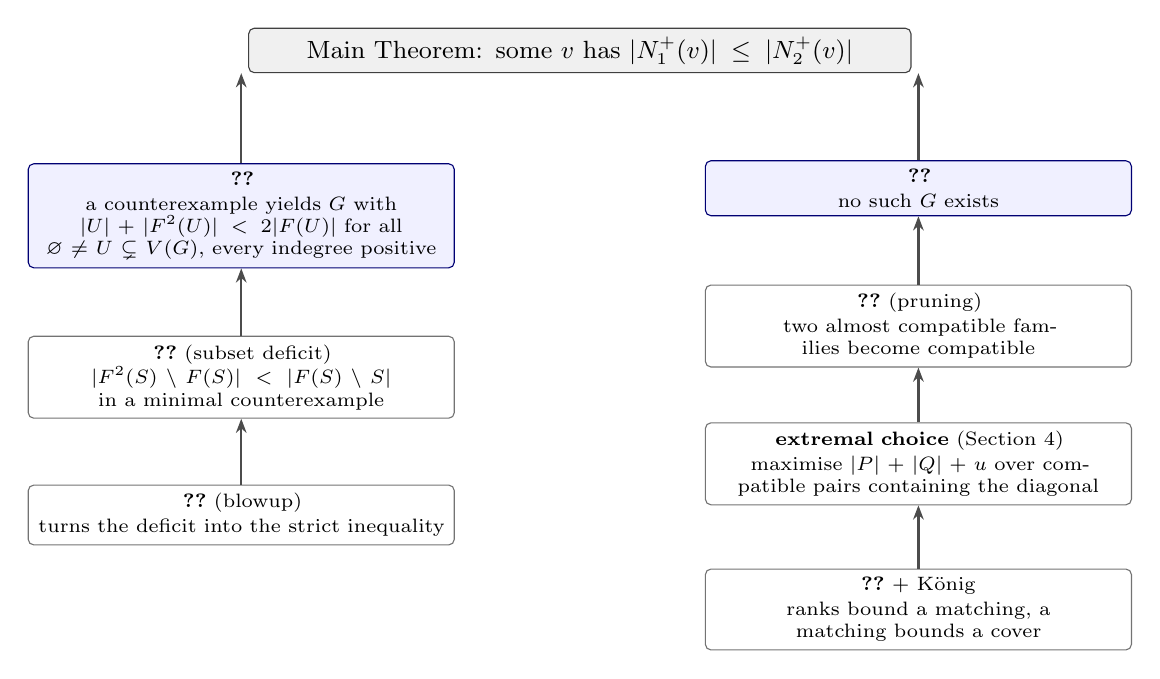
\begin{tikzpicture}[
  box/.style={draw=black!55,fill=white,rounded corners=2pt,align=center,
              font=\scriptsize,inner sep=3pt,text width=#1},
  box/.default=5.2cm,
  thm/.style={box=8.2cm,draw=black!75,fill=black!6,font=\small},
  ar/.style={-{Stealth[length=1.8mm]},draw=black!70,thick}
]
\node[thm] (T) at (0,0) {Main Theorem: some $v$ has $\abs{N_1^+(v)}\le\abs{N_2^+(v)}$};
\node[box,draw=blue!45!black,fill=blue!6] (P2) at (-4.3,-2.1)
  {\textbf{\cref{prop:reduction}}\\[1pt] a counterexample yields $G$ with
   $\abs{U}+\abs{F^2(U)}<2\abs{F(U)}$ for all $\varnothing\ne U\subsetneq V(G)$,
   every indegree positive};
\node[box,draw=blue!45!black,fill=blue!6] (P4) at (4.3,-1.75)
  {\textbf{\cref{prop:no-concavity}}\\[1pt] no such $G$ exists};
\node[box] (L22) at (-4.3,-4.15)
  {\textbf{\cref{lem:deficit}} (subset deficit)\\[1pt]
   $\abs{F^2(S)\setminus F(S)}<\abs{F(S)\setminus S}$ in a minimal counterexample};
\node[box] (L23) at (-4.3,-5.9)
  {\textbf{\cref{lem:blowup}} (blowup)\\[1pt] turns the deficit into the strict inequality};
\node[box] (L31) at (4.3,-3.5)
  {\textbf{\cref{lem:pruning}} (pruning)\\[1pt] two almost compatible families become compatible};
\node[box] (EX) at (4.3,-5.25)
  {\textbf{extremal choice} (Section 4)\\[1pt] maximise $\abs P+\abs Q+u$ over compatible
   pairs containing the diagonal};
\node[box] (L32) at (4.3,-7.1)
  {\textbf{\cref{lem:kernel}} + K\"onig\\[1pt] ranks bound a matching, a matching bounds a cover};
\draw[ar] (P2.north) -- (T.south -| P2.north);
\draw[ar] (P4.north) -- (T.south -| P4.north);
\draw[ar] (L22.north) -- (P2.south);
\draw[ar] (L23.north) -- (L22.south);
\draw[ar] (L31.north) -- (P4.south);
\draw[ar] (EX.north) -- (L31.south);
\draw[ar] (L32.north) -- (EX.south);
\end{tikzpicture}

\caption{The architecture of the proof, read from the bottom up. The main theorem rests on two
 propositions: one converts a counterexample into a graph satisfying a strict subset inequality,
 the other forbids such a graph. Each proposition in turn rests on one substantial lemma.
 \emph{Look at} the two lower boxes: the extremal choice sits between the pruning lemma and the
 contradiction, and is where the two halves of the argument meet. \emph{Why it matters:} \cref{sec:weighted,sec:cycles} are not in this diagram: they consume the
 theorem and produce nothing that is used earlier, so they can be skipped entirely on a first
 reading.}
\label{fig:roadmap}
\end{figure}

\paragraph{How the reduction goes, in words.}
Suppose the theorem fails and take a counterexample $D$ of minimum order, and among those of
minimum number of arcs. Deleting a cleverly chosen family of arcs produces a smaller graph, which
by minimality is \emph{not} a counterexample: some vertex $v$ of it satisfies the desired
inequality. Comparing the neighborhoods of $v$ before and after the deletion shows that the
deleted arcs ``bought'' more second out-neighbors for $v$ than first out-neighbors. Counting this
gain and loss over a chain of deletions, for an arbitrary subset $S$ of vertices, gives the subset
deficit of \cref{lem:deficit}. The blowup then amplifies an integer deficit (at least $1$) into a
margin large enough to survive the final rounding.

\paragraph{How the contradiction goes, in words.}
Represent a \emph{family of ordered pairs} $P\subseteq X\times X$ as a relation: it has a
\emph{column} $P_j=\{p:(p,j)\in P\}$ for each second coordinate and a \emph{row} for each first
coordinate. Advancing the first coordinate along an arc maps $P$ to $\Phi_1P$; advancing the second
coordinate maps a second family $Q$ to $\Phi_2Q$. The families are \emph{compatible} when these two
images are disjoint. Summing the subset inequality over the columns of $P$ and the rows of $Q$ turns
compatibility into a strict inequality between $\abs{P}+\abs{\Phi_1^2P}$ and $2\abs{\Phi_1P}$; taking
complements of the \emph{second} images then produces two families that are worth more than
$M+2u$ but may conflict. The pruning lemma repairs the conflicts at a cost that the uncovered
points pay for. The maximality of $(P,Q)$ is contradicted.

\begin{checkpoint}
After this section you should be able to say, without symbols: \emph{a minimal counterexample
satisfies a strict subset inequality; two families of pairs get pruned to compatibility at a
refundable cost; an extremal pair cannot survive being improved.} Everything that follows is the
proof of one of those three sentences.
\end{checkpoint}

\subsection{History and context}\label{sec:history}

The conjecture was recorded by Dean and Latka~\cite{DeanLatka1995}. The case of
\emph{tournaments} --- oriented graphs with an arc between every two distinct vertices, the case
also known as Dean's conjecture --- was proved by Fisher~\cite{Fisher1996}, using a probability
distribution obtained from Farkas' lemma. Havet and Thomass\'e gave a combinatorial proof using
local median orders~\cite{HavetThomasse2000}. Fidler and Yuster~\cite{FidlerYuster2007} extended
the tournament theorem to tournaments missing a matching, a star, or a clique; Ghazal corrected the
star case and treated generalized stars~\cite{Ghazal2012}. Later extensions cover a matching
together with a star~\cite{DaraFrancisJacobNarayanan2022} and two
stars~\cite{DaamouchAlMninyGhazal2025}.

A second line imposes degree conditions or weakens the ratio. Kaneko and Locke settled the case of
minimum out-degree at most six~\cite{KanekoLocke2001}, and a recent computer-assisted preprint
treats minimum out-degree seven~\cite{SadhukhanSandeepSen2026}. Chen, Shen and
Yuster~\cite{ChenShenYuster2003} proved a universal ratio second-to-first of about $0.657298$;
Huang and Peng~\cite{HuangPeng2024} raise this to about $0.715538$ and report a computational bound
of $0.74530$. Botler, Moura and Naia~\cite{BotlerMouraNaia2023}, followed by Espuny D\'iaz,
Gir\~ao, Granet and Kronenberg~\cite{EspunyDiazEtAl2025}, treated every orientation of a binomial
random graph; the latter covers every fixed edge probability below $1/2$ with probability tending
to one. Brukhman's recent dense-case preprint~\cite{Brukhman2026} concerns order $n\le 2\delta+2$,
where $\delta$ is the minimum out-degree.

The present proof builds on the minimal-counterexample and graph-product methods of Brantner,
Brockman, Kay and Snively~\cite{BrantnerBrockmanKaySnively2009} and on Seacrest's subset
perspective~\cite{Seacrest2019}. It adapts the edge-deletion idea in the proof of Seacrest's
Lemma~4 --- specializing his parameter to $1$ --- to obtain the stronger subset inequality needed
here, and gives that argument in full. The main additional ingredient is the pruning bound for
arbitrary finite binary relations (\cref{lem:pruning}), whose deletion cost depends on the points
left uncovered after pruning.

\subsection{Organization of the paper}\label{sec:organisation}

\begin{description}[leftmargin=1.4em,itemsep=2pt]
\item[\Cref{sec:reduction}] From a counterexample to a strict subset inequality
  (\cref{prop:reduction}), via the subset deficit (\cref{lem:deficit}) and the blowup
  (\cref{lem:blowup}). This is the \emph{first engine} and the easiest of the three to read.
\item[\Cref{sec:pruning}] The pruning lemma (\cref{lem:pruning}) for arbitrary finite binary
  relations, and the rank lemma (\cref{lem:kernel}) that makes it work. This is the \emph{second
  engine}; it is independent of graph theory and can be read on its own.
\item[\Cref{sec:incompatibility}] The extremal contradiction (\cref{prop:no-concavity}). This is
  the \emph{third engine} and the place where the first two meet.
\item[\Cref{sec:weighted,sec:cycles}] Consequences: the vertex- and arc-weighted forms via
  Seacrest's equivalences, and consequences for directed triangles, minimum degree and girth.
  Neither is used in the proof of \cref{thm:main}.
\item[\appref{app:toolkit}] The five facts used from outside graph theory, with proofs: K\H{o}nig's
  theorem, rank--nullity, Sylvester's inequality, the minor--matching bound, and the Farkas
  alternative. Nothing in the main text depends on anything else.
\item[\appref{app:alternatives}] What was tried in search of a shorter proof: two simplifications that
  were adopted (no Edmonds, no Seacrest for the vertex-weighted forms) and four attempts that failed,
  with the reason.
\item[Appendices~\ref{app:depgraph}, \ref{app:dictionary} and \ref{app:checks}] A dependency graph of the numbered statements,
  a dictionary of notation against the original preprint, and a record of how each step was
  checked (re-derivation, exhaustive computation on small cases, and a Lean formalisation).
\end{description}

\section{From a counterexample to a strict subset inequality}\label{sec:reduction}

\begin{contract}
\textbf{Assumes:} that \cref{thm:main} has a counterexample. \quad
\textbf{Produces:} an oriented graph $G$, all of whose indegrees are positive, satisfying the
strict inequality
\[
 \abs{U}+\abs{F_G^2(U)}<2\abs{F_G(U)}
 \qquad\text{for every nonempty proper }U\subseteq V(G).
\]
\textbf{Why:} this is the graph that \cref{sec:incompatibility} destroys. The section is the
\emph{first engine}: a minimal counterexample is forced to satisfy a strictly stronger, purely
set-theoretic inequality, and a blowup amplifies the integer margin so that later rounding cannot
lose it.
\end{contract}

Throughout, $F=F_D$ is the \emph{union of out-neighborhoods} in a graph $D$:
\begin{equation}\label{eq:Fdef}
 F(S)=\{y\in V(D):\ \text{there is }x\in S\text{ with }x\to y\},
 \qquad F^k(S)=\underbrace{F(F(\cdots F}_{k}(S)\cdots)).
\end{equation}
Two warnings about \eqref{eq:Fdef}, both used constantly. First, $F(S)$ does \emph{not} subtract
$S$: an arc inside $S$ keeps its head in $F(S)$. Second, $F^2(\{v\})$ does \emph{not} exclude $v$;
what excludes $v$ is the orientation. In an oriented graph there is no two-step walk from $v$ back
to $v$ (that would need $v\to u\to v$, two opposite arcs), so
\begin{equation}\label{eq:N2equals}
 N_2^+(v)=F^2(\{v\})\setminus F(\{v\}),
\end{equation}
with no need to remove $v$ separately. The two operators $F$ and $N_2^+$ are the same object seen
from two angles: $F$ acts on sets of vertices, $N_2^+$ is the special case of a single vertex, with
the first neighborhood subtracted.

The goal of the section is the following.

\begin{proposition}[Counterexample reduction]\label{prop:reduction}
If \cref{thm:main} has a counterexample, then there is a finite nonempty oriented graph $G$ in which
every vertex has positive indegree and
\begin{equation}\label{eq:strict-growth}
 \abs{U}+\abs{F_G^2(U)}<2\abs{F_G(U)}
 \qquad\text{for every }\varnothing\ne U\subsetneq V(G).
\end{equation}
\end{proposition}

\inwords{If the conjecture fails somewhere, then somewhere else there is a graph in which every
nonempty proper set of vertices has its second image strictly smaller than the average of the set
and its first image.}

\begin{planbox}
\begin{enumerate}[leftmargin=1.3em,itemsep=1pt,topsep=1pt]
\item \textbf{Subset deficit} (\cref{lem:deficit}): in a counterexample chosen minimal first by
  order and then by number of arcs, every nonempty proper $S$ satisfies the \emph{strict} deficit
  $\abs{F^2(S)\setminus F(S)}<\abs{F(S)\setminus S}$. The right-hand side is the part of the first
  image that lies outside $S$; that refinement is what makes the rest work.
\item \textbf{Blowup} (\cref{lem:blowup}): replacing every vertex by a transitive tournament on
  $m>\abs{V(D)}$ vertices multiplies the deficit by $m$ and costs at most $n$ in rounding, turning
  an integer deficit (at least $1$) into \eqref{eq:strict-growth}.
\end{enumerate}
\end{planbox}

\begin{proof}[Proof of \cref{prop:reduction}, assuming \cref{lem:deficit} and \cref{lem:blowup}]
Choose a counterexample $D$ of minimum order, and among those of minimum number of arcs.
\Cref{lem:deficit} supplies positive indegrees for $D$ and the deficit
$\abs{F^2(S)\setminus F(S)}<\abs{F(S)\setminus S}$ for every nonempty proper $S$. Apply
\cref{lem:blowup} with any integer $m>\abs{V(D)}$; the resulting $G$ is as required.
\end{proof}

\subsection{The subset deficit}\label{sec:deficit}

\begin{ideabox}
The conjecture says $\abs{N_2^+(v)}<\abs{N_1^+(v)}$ at every vertex of a counterexample. We want a
statement about \emph{sets} of vertices rather than single vertices, and we want it to be strict
with a robust right-hand side. The device that produces it is: delete the arcs from $S$ to a
carefully chosen part of $E=F(S)\setminus S$, and see what minimality says about the vertex that
must now satisfy the inequality. Deleting arcs can only shrink first neighborhoods and can only
shrink second neighborhoods; so the vertex that gains from the deletion must have \emph{lost} some
out-neighbors, and the bookkeeping of that trade is the content of the lemma.
\end{ideabox}

\begin{lemma}[Subset deficit]\label{lem:deficit}
Let $D$ be a finite nonempty oriented graph with $\abs{N_1^+(v)}>\abs{N_2^+(v)}$ for every
$v\in V(D)$, chosen with minimum order and, subject to that, with minimum number of arcs. Then $D$
is strongly connected, every vertex has positive indegree, and
\begin{equation}\label{eq:deficit}
 \abs{F^2(S)\setminus F(S)}<\abs{F(S)\setminus S}
 \qquad\text{for every }\varnothing\ne S\subsetneq V(D).
\end{equation}
\end{lemma}

\inwords{In a smallest counterexample, every proper nonempty set $S$ loses, at its second image,
strictly less than the size of the part of its first image that lies outside $S$.}

\usedin{This is the only place where minimality of the counterexample is used; it feeds
\cref{lem:blowup} and hence \cref{prop:reduction}}

\begin{planbox}
\begin{enumerate}[leftmargin=1.3em,itemsep=1pt,topsep=1pt]
\item \textbf{Clean up the graph} (Step~1): no sink, at least two vertices, strongly
  connected, all indegrees positive.
\item \textbf{Fix $S$ and split the first image} (Step~2): $I=F(S)\cap S$ is the
  \emph{internal} part, $E=F(S)\setminus S$ the \emph{external} part; $E\ne\varnothing$. Define
  $g(Y)=\abs{F(Y)\setminus(I\cup Y)}$ for $Y\subseteq E$, so that the target inequality reads
  $g(E)<\abs E$.
\item \textbf{Build a deletion machine} (Step~3): for $Y\subsetneq E$, delete all arcs
  from $S$ to $E\setminus Y$. Minimality of the arc count gives a vertex $v$ satisfying the
  inequality in the smaller graph; show $v\in S$, and let $Q_v$ be the out-neighbors it loses.
\item \textbf{Do the bookkeeping} (Step~4): the second out-neighborhood of $v$ loses
  exactly a set $\Lambda$ and gains only points of $Q_v\cap F(Y)$; hence the increase of $g$ is
  less than $\abs{Q_v}$.
\item \textbf{Iterate} (Step~5) from $Y=\varnothing$ to $Y=E$, and sum.
\end{enumerate}
\end{planbox}

\begin{proof}
\steplabel{Step 1: the graph is strongly connected.}
A sink satisfies $\abs{N_1^+(v)}=0\le\abs{N_2^+(v)}$, so $D$ has no sink; in particular $D$ is not
a single vertex, since a single vertex is a sink. If $D$ were not strongly connected, its
condensation would have a sink component $C$: a strongly connected component with no arc to
another component. Every out-neighbor, and therefore every two-step out-neighbor, of a vertex of
$C$ lies in $C$. Hence $D[C]$ would be a counterexample of smaller order, contradicting minimality.
So $D$ is strongly connected, and since it has more than one vertex, every vertex has an
in-neighbor.

\steplabel{Step 2: fix a subset and split its first image.}
Let $\varnothing\ne S\subsetneq V(D)$ and put
\begin{equation}\label{eq:IE}
 I=F(S)\cap S,\qquad E=F(S)\setminus S,\qquad F(S)=I\sqcup E,
\end{equation}
and, for $Y\subseteq E$,
\begin{equation}\label{eq:gdef}
 g(Y)=\abs{F(Y)\setminus(I\cup Y)} .
\end{equation}
We have $E\ne\varnothing$: otherwise $S$ would have no arc to $V(D)\setminus S$, contradicting
strong connectivity as $S$ is nonempty and proper. The reader should keep \cref{fig:deficit} in
mind: $I$ is the part of the first image that falls back inside $S$, $E$ the part that falls
outside.

\begin{figure}[t]
\centering
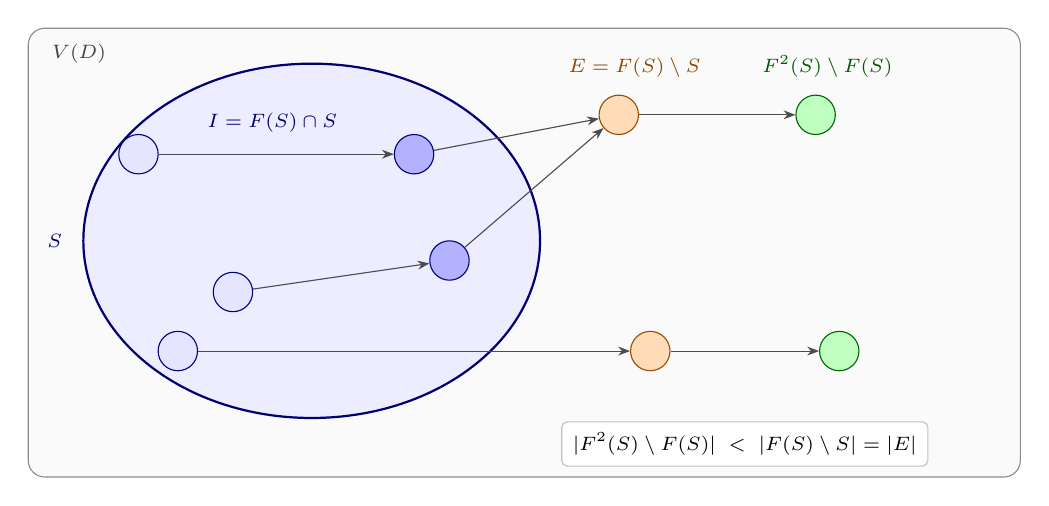
\begin{tikzpicture}[
  svert/.style={circle,draw=blue!50!black,fill=blue!10,inner sep=0pt,minimum size=5mm,font=\scriptsize},
  ivert/.style={circle,draw=blue!50!black,fill=blue!30,inner sep=0pt,minimum size=5mm,font=\scriptsize},
  evert/.style={circle,draw=orange!60!black,fill=orange!28,inner sep=0pt,minimum size=5mm,font=\scriptsize},
  gvert/.style={circle,draw=green!40!black,fill=green!25,inner sep=0pt,minimum size=5mm,font=\scriptsize},
  arc/.style={-{Stealth[length=1.5mm]},draw=black!70},
  lab/.style={font=\scriptsize,text=black!75}
]
% ambient box
\draw[draw=black!45,rounded corners=6pt,fill=black!2] (0,0) rectangle (12.6,5.7);
\node[lab,anchor=north west] at (0.18,5.62) {$V(D)$};
% S
\draw[blue!45!black,fill=blue!7,thick] (3.6,3.0) ellipse (2.9 and 2.25);
\node[lab,text=blue!45!black,anchor=west] at (0.12,3.0) {$S$};
% vertices
\node[svert] (s1) at (1.4,4.1) {};
\node[svert] (s2) at (1.9,1.6) {};
\node[svert] (s3) at (2.6,2.35) {};
\node[ivert] (i1) at (4.9,4.1) {};
\node[ivert] (i2) at (5.35,2.75) {};
\node[evert] (e1) at (7.5,4.6) {};
\node[evert] (e2) at (7.9,1.6) {};
\node[gvert] (g1) at (10.0,4.6) {};
\node[gvert] (g2) at (10.3,1.6) {};
% arcs
\draw[arc] (s1) -- (i1);
\draw[arc] (s3) -- (i2);
\draw[arc] (i2) -- (e1);
\draw[arc] (i1) -- (e1);
\draw[arc] (e1) -- (g1);
\draw[arc] (s2) -- (e2);
\draw[arc] (e2) -- (g2);
% region labels, all clear of nodes and arcs
\node[lab,text=blue!45!black,anchor=south] at (3.1,4.25) {$I=F(S)\cap S$};
\node[lab,text=orange!55!black,anchor=south] at (7.7,4.95) {$E=F(S)\setminus S$};
\node[lab,text=green!35!black,anchor=south] at (10.15,4.95) {$F^2(S)\setminus F(S)$};
% the inequality, on a plate below the ellipse
\node[draw=black!25,fill=white,rounded corners=2pt,inner sep=4pt,font=\scriptsize]
  at (9.1,0.42) {$\abs{F^2(S)\setminus F(S)} \;<\; \abs{F(S)\setminus S}=\abs E$};
\end{tikzpicture}

\caption{The split \eqref{eq:IE} of the first image of $S$. \emph{Look at} the three regions: $I$
 (the first image that stays inside $S$), $E$ (the first image outside $S$), and the region
 $F^2(S)\setminus F(S)$ (second image not already seen in one step). \emph{Why it matters:}
 \cref{lem:deficit} compares the size of the third region with the size of $E$, not with the size
 of $F(S)=I\sqcup E$. The part $I$ is free: it is already ``paid for'' by $S$.}
\label{fig:deficit}
\end{figure}

Note the two extremes: $g(\varnothing)=0$, and $g(E)=\abs{F(E)\setminus(I\cup E)}$. Since
$F(S)=I\sqcup E$ and $F(I)\subseteq F(S)=I\sqcup E$, we shall be able to identify the target
quantity at the end:
\begin{equation}\label{eq:deficit-via-g}
 F^2(S)\setminus F(S)
 =\bigl(F(I)\cup F(E)\bigr)\setminus(I\cup E)
 =F(E)\setminus(I\cup E),
\end{equation}
so that $\abs{F^2(S)\setminus F(S)}=g(E)$.

\steplabel{Step 3: the deletion machine.}
Fix $Y\subsetneq E$. Let $D_Y$ be the graph obtained from $D$ by deleting \emph{all} arcs from $S$
to $E\setminus Y$; all other arcs are kept. Every vertex of $E\setminus Y$ has an in-neighbor in
$S$, because $E\setminus Y\subseteq E=F(S)\setminus S$; so at least one arc is deleted and $D_Y$
has strictly fewer arcs than $D$.

Minimality of the number of arcs (the order is unchanged) says that $D_Y$ is \emph{not} a
counterexample. So there is a vertex $v$ with
\begin{equation}\label{eq:DY-inequality}
 \abs{N_{1,D_Y}^+(v)}\le\abs{N_{2,D_Y}^+(v)}.
\end{equation}
If $v$ had lost no out-neighbor, then $N_{1,D_Y}^+(v)=N_1^+(v)$ while $N_{2,D_Y}^+(v)\subseteq
N_2^+(v)$ (deleting arcs creates no paths), so
$\abs{N_{2,D_Y}^+(v)}\le\abs{N_2^+(v)}<\abs{N_1^+(v)}=\abs{N_{1,D_Y}^+(v)}$, contradicting
\eqref{eq:DY-inequality}. Hence $v$ lost an out-neighbor, which means $v\in S$: only arcs with tail
in $S$ were deleted. Put
\begin{equation}\label{eq:Qv}
 Q_v=F(\{v\})\cap(E\setminus Y)=\{\text{out-neighbors of }v\text{ that }D_Y\text{ does not have}\}.
\end{equation}
Then $Q_v\ne\varnothing$, and $Q_v$ is disjoint from $I\cup Y$ because $Q_v\subseteq E\setminus Y$
and $Y\subseteq E$ is disjoint from $S\supseteq I$. Also $F(\{v\})\subseteq I\cup Y\cup Q_v$,
since $F(\{v\})\subseteq F(S)=I\sqcup E$.

\steplabel{Step 4: what $v$ loses and what it gains.}
\Cref{fig:deletion} shows the four sets involved. We record four facts.

\emph{(4a) The second image after deletion is confined.} Since $v\in S$, its out-neighbors in
$D_Y$ lie in $I\cup Y$; and for such an out-neighbor $x$,
\begin{itemize}[leftmargin=1.4em,itemsep=1pt,topsep=1pt]
\item if $x\in I\subseteq S$, then all arcs out of $x$ into $E\setminus Y$ were deleted, so
  $F_{D_Y}(x)\subseteq F(x)\setminus(E\setminus Y)\subseteq (I\sqcup E)\setminus(E\setminus
  Y)=I\cup Y$;
\item if $x\in Y$, then $F_{D_Y}(x)\subseteq F(x)\subseteq F(Y)$.
\end{itemize}
Hence
\begin{equation}\label{eq:confined}
 F_{D_Y}^2(\{v\})\subseteq I\cup Y\cup F(Y).
\end{equation}

\emph{(4b) New second out-neighbors are first out-neighbors.} A vertex counted in
$N_{2,D_Y}^+(v)$ but not in $N_2^+(v)$ is the end of a two-step path of $D_Y$, hence of $D$; it is
not a first out-neighbor in $D_Y$. So it was a first out-neighbor in $D$, i.e.\ it lies in $Q_v$;
and by \eqref{eq:confined} it lies in $I\cup Y\cup F(Y)$. As $Q_v$ misses $I\cup Y$,
\begin{equation}\label{eq:new}
 N_{2,D_Y}^+(v)\setminus N_2^+(v)\subseteq Q_v\cap F(Y).
\end{equation}

\emph{(4c) The set $\Lambda$ is lost.} Define
\begin{equation}\label{eq:Lambda}
 \Lambda=F(Q_v)\setminus\bigl(I\cup Y\cup Q_v\cup F(Y)\bigr).
\end{equation}
Each $y\in\Lambda$ has $v\to q\to y$ with $q\in Q_v\subseteq F(\{v\})$, so $y\in F^2(\{v\})$. Also
$y\notin F(\{v\})$, because $F(\{v\})\subseteq I\cup Y\cup Q_v$; and $y\ne v$, because $y\in F(Q_v)$
and an arc $q\to v$ would be opposite to the arc $v\to q$. Hence
\begin{equation}\label{eq:Lambda-sub}
 \Lambda\subseteq N_2^+(v).
\end{equation}
On the other hand $\Lambda\cap(I\cup Y\cup F(Y))=\varnothing$ by definition, so \eqref{eq:confined}
gives $\Lambda\cap N_{2,D_Y}^+(v)=\varnothing$: every point of $\Lambda$ was counted before the
deletion and is not counted after it.

\emph{(4d) The change of $g$ is exact.} Since $F(Y\cup Q_v)=F(Y)\cup F(Q_v)$,
\begin{align}
 F(Y\cup Q_v)\setminus(I\cup Y\cup Q_v)
 &=\bigl(F(Y)\setminus(I\cup Y\cup Q_v)\bigr)
   \;\sqcup\;\bigl(F(Q_v)\setminus(I\cup Y\cup Q_v\cup F(Y))\bigr)\notag\\
 &=\bigl(F(Y)\setminus(I\cup Y)\bigr)\setminus Q_v\;\;\sqcup\;\;\Lambda,
 \label{eq:g-change}
\end{align}
using $Q_v\cap(I\cup Y)=\varnothing$ in the second line. Therefore
\begin{equation}\label{eq:g-diff}
 g(Y\cup Q_v)-g(Y)=\abs\Lambda-\abs{Q_v\cap F(Y)}.
\end{equation}

Now put $d_1=\abs{N_1^+(v)}$ and $d_2=\abs{N_2^+(v)}$, the degrees \emph{in $D$}. By definition of
$Q_v$ the first out-neighborhood loses exactly $Q_v$:
\begin{equation}\label{eq:first-loss}
 \abs{N_{1,D_Y}^+(v)}=d_1-\abs{Q_v}.
\end{equation}
By \eqref{eq:Lambda-sub} and \eqref{eq:confined}, the second out-neighborhood can only lose points
of $\Lambda$ and can only gain points of $Q_v\cap F(Y)$:
\begin{equation}\label{eq:second-change}
 \abs{N_{2,D_Y}^+(v)}\le d_2-\abs\Lambda+\abs{Q_v\cap F(Y)}.
\end{equation}
Substituting \eqref{eq:first-loss} and \eqref{eq:second-change} into \eqref{eq:DY-inequality},
\begin{equation}\label{eq:increment-bound}
 \abs\Lambda-\abs{Q_v\cap F(Y)}
 \overset{\eqref{eq:g-diff}}{=}g(Y\cup Q_v)-g(Y)
 \le \abs{Q_v}+d_2-d_1<\abs{Q_v},
\end{equation}
where the last inequality is the counterexample hypothesis $d_2<d_1$.

\steplabel{Step 5: iterate and sum.}
Start with $Y_0=\varnothing$ and, as long as $Y_i\ne E$, apply Step 3--4 to $Y_i$ to obtain
$Q_{v_i}\ne\varnothing$ with $Q_{v_i}\subseteq E\setminus Y_i$, and set $Y_{i+1}=Y_i\cup Q_{v_i}$.
The sets $Y_i$ strictly increase inside the finite set $E$, so the process stops, and it can only
stop at $Y_r=E$. Each step is performed afresh on the \emph{original} $D$, so minimality applies at
every step. Summing \eqref{eq:increment-bound} over the steps and telescoping,
\[
 g(E)-g(\varnothing)=\sum_{i=0}^{r-1}\bigl(g(Y_{i+1})-g(Y_i)\bigr)<\sum_{i=0}^{r-1}\abs{Q_{v_i}}
 =\abs{E},
\]
because the $Q_{v_i}$ partition $E$. As $g(\varnothing)=0$ and, by \eqref{eq:deficit-via-g},
$g(E)=\abs{F^2(S)\setminus F(S)}$ while $\abs E=\abs{F(S)\setminus S}$, this is
\eqref{eq:deficit}. As $S$ was arbitrary, the lemma is proved.
\end{proof}

\begin{figure}[t]
\centering
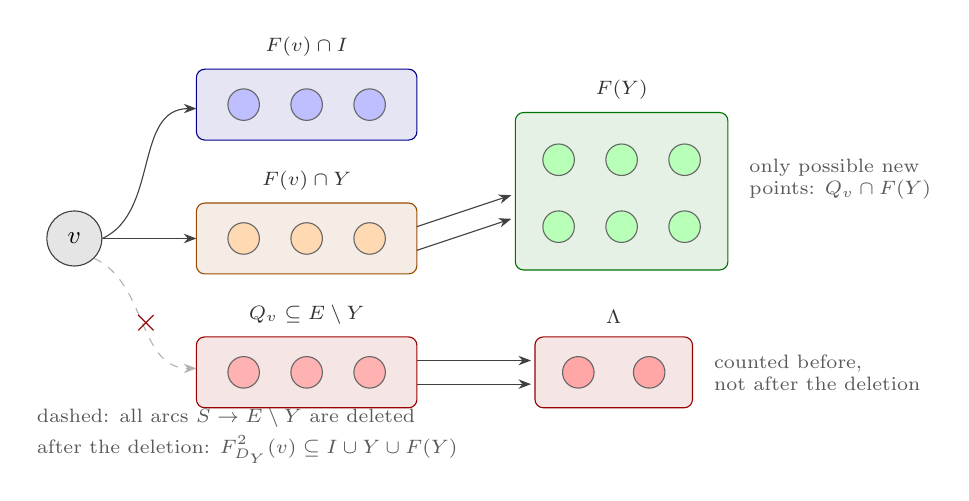
\begin{tikzpicture}[
  dot/.style={circle,draw=black!60,fill=#1,inner sep=0pt,minimum size=4mm},
  dot/.default=black!10,
  grp/.style={draw=#1,fill=#1!10,rounded corners=3pt},
  grp/.default=black!40,
  arc/.style={-{Stealth[length=1.6mm]},draw=black!75},
  del/.style={-{Stealth[length=1.6mm]},draw=black!30,dashed},
  lab/.style={font=\scriptsize,text=black!80},
  annot/.style={font=\scriptsize,text=black!65,align=left}
]
% v
\node[circle,draw=black!75,fill=black!10,inner sep=0pt,minimum size=7mm,font=\small] (v) at (0.7,2.8) {$v$};
% three groups of out-neighbours (drawn as boxes, labels above)
\draw[grp=blue!55!black] (2.25,4.05) rectangle (5.05,4.95);
\node[lab,anchor=south] at (3.65,4.99) {$F(v)\cap I$};
\node[dot=blue!25] at (2.85,4.5) {}; \node[dot=blue!25] at (3.65,4.5) {}; \node[dot=blue!25] at (4.45,4.5) {};
\draw[grp=orange!60!black] (2.25,2.35) rectangle (5.05,3.25);
\node[lab,anchor=south] at (3.65,3.29) {$F(v)\cap Y$};
\node[dot=orange!30] at (2.85,2.8) {}; \node[dot=orange!30] at (3.65,2.8) {}; \node[dot=orange!30] at (4.45,2.8) {};
\draw[grp=red!60!black] (2.25,0.65) rectangle (5.05,1.55);
\node[lab,anchor=south] at (3.65,1.59) {$Q_v\subseteq E\setminus Y$};
\node[dot=red!30] at (2.85,1.1) {}; \node[dot=red!30] at (3.65,1.1) {}; \node[dot=red!30] at (4.45,1.1) {};
% kept and deleted arcs out of v
\draw[arc] (v.east) to[out=25,in=180] (2.25,4.45);
\draw[arc] (v.east) to[out=0,in=180]  (2.25,2.8);
\draw[del] (v.south east) to[out=-25,in=180] (2.25,1.15);
\node[font=\large,text=red!55!black] at (1.62,1.72) {$\times$};
% F(Y) and Lambda
\draw[grp=green!45!black] (6.3,2.4) rectangle (9.0,4.4);
\node[lab,anchor=south] at (7.65,4.44) {$F(Y)$};
\node[dot=green!28] at (6.85,3.8) {}; \node[dot=green!28] at (7.65,3.8) {}; \node[dot=green!28] at (8.45,3.8) {};
\node[dot=green!28] at (6.85,2.95) {}; \node[dot=green!28] at (7.65,2.95) {}; \node[dot=green!28] at (8.45,2.95) {};
\draw[grp=red!60!black] (6.55,0.65) rectangle (8.55,1.55);
\node[lab,anchor=south] at (7.55,1.59) {$\Lambda$};
\node[dot=red!35] at (7.1,1.1) {}; \node[dot=red!35] at (8.0,1.1) {};
% arcs into F(Y) and Lambda
\draw[arc] (5.05,2.95) -- (6.25,3.35);
\draw[arc] (5.05,2.65) -- (6.25,3.05);
\draw[arc] (5.05,1.25) -- (6.5,1.25);
\draw[arc] (5.05,0.95) -- (6.5,0.95);
% side annotations
\node[annot,anchor=west] at (9.15,3.55) {only possible new\\ points: $Q_v\cap F(Y)$};
\node[annot,anchor=west] at (8.7,1.1) {counted before,\\ not after the deletion};
% legend, clear of everything
\node[annot,anchor=west] at (0.1,0.52) {dashed: all arcs $S\to E\setminus Y$ are deleted};
\node[annot,anchor=west] at (0.1,0.12) {after the deletion: $F_{D_Y}^2(v)\subseteq I\cup Y\cup F(Y)$};
\end{tikzpicture}

\caption{The deletion step of \cref{lem:deficit}. \emph{Look at} the crossed-out arcs on the left:
 all arcs from $S$ to $E\setminus Y$ are deleted, so the out-neighbors of $v$ that lie in $Q_v$
 disappear, and with them every two-step path that used one of them. \emph{Why it matters:} the
 second out-neighborhood is confined to $I\cup Y\cup F(Y)$ after the deletion
 \eqref{eq:confined}; the points of $\Lambda$ (bottom right) were counted before and are not
 counted after, while the only points that can be gained are the points of $Q_v\cap F(Y)$ ---
 which are also first out-neighbors of $v$, hence are paid for by the first loss.}
\label{fig:deletion}
\end{figure}

\begin{remark}[The ledger, and why the right-hand side is $\abs{F(S)\setminus S}$]\label{rem:ledger}
The four facts of Step 4 are best remembered as a table of what happens to the two neighborhoods of
$v$ when the arcs from $S$ to $E\setminus Y$ are deleted.

\begin{center}
\small
\renewcommand{\arraystretch}{1.25}
\begin{tabular}{@{}llll@{}}
\toprule
quantity & in $D$ & in $D_Y$ & reason \\
\midrule
$\abs{N_1^+(v)}$ & $d_1$ & $d_1-\abs{Q_v}$ & loses exactly $Q_v$, \eqref{eq:first-loss}\\
$\abs{N_2^+(v)}$ & $d_2$ & $\le d_2-\abs\Lambda+\abs{Q_v\cap F(Y)}$ & \eqref{eq:Lambda-sub}, \eqref{eq:confined}, \eqref{eq:new}\\
$g(Y)$ & $g(Y)$ & $g(Y)+\abs\Lambda-\abs{Q_v\cap F(Y)}$ & exact, \eqref{eq:g-diff}\\
\bottomrule
\end{tabular}
\end{center}

Two remarks explain the shape of the lemma.

\emph{(i) The gain is charged to the first out-neighbors.} The new second out-neighbors lie in
$Q_v\cap F(Y)\subseteq Q_v$, and $Q_v$ is precisely the set of first out-neighbors that the
deletion removed. This is why the increment is bounded by $\abs{Q_v}$ and not by $\abs{N_1^+(v)}$:
the deletion pays for the gain out of the first neighborhood, and the deficit $d_2<d_1$ supplies the
strictness.

\emph{(ii) Why $I$ does not appear on the right-hand side.} If the right-hand side of
\eqref{eq:deficit} were $\abs{F(S)}$, the display \eqref{eq:g-diff} would have to account for
$I$ as well, and $I$ is not controlled by the deletion at all. Working with
$F(S)\setminus S=E$ means that the internal part of the image is simply not part of the ledger.
\end{remark}

\subsection{The blowup}\label{sec:blowup}

\begin{ideabox}
\Cref{eq:deficit} has an integer left-hand side and an integer right-hand side, so it gives a
margin of at least $1$. The final argument, however, needs the inequality $\abs{U}+\abs{F^2(U)}<
2\abs{F(U)}$ to survive a comparison in which a term of size at most $n$ (the number of base
vertices) competes with the margin. Replacing every vertex by many twins multiplies the margin by
the block size $m$ while the rounding error stays at $n$: choose $m>n$ and the margin wins.
\end{ideabox}

\begin{lemma}[Transitive-tournament blowup]\label{lem:blowup}
Let $D$ be an oriented graph on $n\ge1$ vertices, all of positive indegree, satisfying
\eqref{eq:deficit} for every nonempty proper subset of $V(D)$. Let $m>n$ be an integer. Replace
every vertex of $D$ by a transitive tournament on $m$ vertices; for every arc $v\to w$ of $D$ put
\emph{all} arcs from the block of $v$ to the block of $w$, and put no other arcs between distinct
blocks. Then the resulting graph $G$ is oriented, all its indegrees are positive, and
\[
 \abs{U}+\abs{F_G^2(U)}<2\abs{F_G(U)}
 \qquad\text{for every }\varnothing\ne U\subsetneq V(G).
\]
\end{lemma}

\inwords{Putting a large transitive tournament in place of each vertex multiplies the subset deficit
by the block size, which beats the rounding error.}

\usedin{Combined with \cref{lem:deficit} it gives \cref{prop:reduction}, hence the hypothesis of
\cref{prop:no-concavity}}

\begin{planbox}
\begin{enumerate}[leftmargin=1.3em,itemsep=1pt,topsep=1pt]
\item \textbf{Internal accounting} (Step~1): inside one block, a nonempty set $T$ of
  labels has image $\tau(T)=\{a+1,\dots,m\}$ where $a=\min T$; hence $\abs T-\abs{\tau(T)}\le1$,
  $\tau^2(T)\subseteq\tau(T)$ and $\abs T-2\abs{\tau(T)}+\abs{\tau^2(T)}\le1$.
\item \textbf{External accounting} (Step~3): if $U$ meets exactly the blocks in $S$, then
  every block indexed by $F(S)$ is \emph{completely} contained in $F_G(U)$, and every block
  indexed by $F^2(S)$ is completely contained in $F_G^2(U)$.
\item \textbf{The ledger} (Step~4): combine the two accounts; the coefficient of $m$ is
  exactly $\abs{F^2(S)\setminus F(S)}-\abs{F(S)\setminus S}\le-1$, and everything else is at most
  $n$.
\item \textbf{The case $S=V(D)$} (Step~5), where the hypothesis \eqref{eq:deficit} is not
  available and a separate argument is needed.
\end{enumerate}
\end{planbox}

\begin{proof}
\steplabel{Step 1: inside a block.}
Write $V(G)=V(D)\times\{1,\dots,m\}$, with the block of $v$ being $\{v\}\times\{1,\dots,m\}$, and
put an arc from $(v,a)$ to $(v,b)$ exactly when $a<b$. Let $\tau$ be the image operator of this
transitive tournament: for $T\subseteq\{1,\dots,m\}$,
\begin{equation}\label{eq:tau}
 \tau(T)=\{b:\ \exists a\in T,\ a<b\}
 =\begin{cases}\{a+1,\dots,m\},&a=\min T,\ T\ne\varnothing,\\ \varnothing,&T=\varnothing.\end{cases}
\end{equation}
For nonempty $T$ with $a=\min T$ we have $T\subseteq\{a,\dots,m\}$ and $\tau(T)=\{a+1,\dots,m\}$,
so
\begin{equation}\label{eq:tau-bounds}
 \abs T-\abs{\tau(T)}\le1,\qquad
 \tau^2(T)\subseteq\tau(T),\qquad
 \abs T-2\abs{\tau(T)}+\abs{\tau^2(T)}\le1 .
\end{equation}
(The inclusion is immediate from \eqref{eq:tau}. The first inequality says that $T$ contains at
most one label below $\tau(T)$; the second that $\tau(T)$ is an interval ending at $m$, so its own
image is smaller still.)

\steplabel{Step 2: the construction is oriented with positive indegrees.}
Inside a block the arcs are transitive, so no loops and no opposite pairs; between two blocks the
arcs all point one way, determined by the arc of $D$; and there is no arc between non-adjacent
blocks. So $G$ is oriented. A vertex $(v,a)$ receives arcs from every block $\{u\}\times\{1,\dots,m\}$
with $u\to v$ in $D$, and every vertex of $D$ has an in-neighbor by hypothesis; so every indegree in
$G$ is positive.

\steplabel{Step 3: which blocks are completely covered.}
Fix a nonempty proper $U\subseteq V(G)$ and let
\begin{equation}\label{eq:support}
 \begin{gathered}
  T_v=\{a:(v,a)\in U\}\subseteq\{1,\dots,m\},\qquad
  S=\{v\in V(D):T_v\ne\varnothing\},\\
  W=F(S)\cup F^2(S).
 \end{gathered}
\end{equation}
\Cref{fig:blowup} shows the three kinds of blocks. First, \emph{every block indexed by $F(S)$ is
completely contained in $F_G(U)$}: if $w\in F(S)$ there is $v\in S$ with $v\to w$, and then
$(v,a)\to(w,b)$ for \emph{all} $a,b$, so the whole block of $w$ is reached. In a block $w\notin
F(S)$ there are no arcs from $U$ into it, so its contribution to $F_G(U)$ is exactly the internal
image $\tau(T_w)$. Therefore
\begin{equation}\label{eq:FG}
 \abs{F_G(U)}=m\,\abs{F(S)}+\sum_{v\in S\setminus F(S)}\abs{\tau(T_v)} .
\end{equation}
Second, \emph{every block indexed by $F^2(S)$ is completely contained in $F_G^2(U)$}: a two-step
path from $U$ whose two steps are external ends anywhere in a block of $F(F(S))=F^2(S)$. A
two-step path with exactly one external step lands in a block of $F(S)$ (if the external step is
the second) or stays inside a block of $F(S)$ (if it is the first, and the block is already full).
A two-step path with no external step contributes $\tau^2(T_v)$ inside the block of $v$. Since
blocks indexed by $F(S)\subseteq W$ are already fully counted,
\begin{equation}\label{eq:FG2}
 \abs{F_G^2(U)}\le m\,\abs W+\sum_{v\in S\setminus W}\abs{\tau^2(T_v)} .
\end{equation}

\steplabel{Step 4: the ledger.}
Subtracting twice \eqref{eq:FG} from \eqref{eq:FG2} and adding $\abs U=\sum_{v\in S}\abs{T_v}$,
\begin{align}
 \abs U-2\abs{F_G(U)}+\abs{F_G^2(U)}
 &\le m\bigl(\abs W-2\abs{F(S)}\bigr)+\sum_{v\in S}\abs{T_v}\notag\\
 &\qquad{}-2\!\!\sum_{v\in S\setminus F(S)}\!\!\abs{\tau(T_v)}
       +\sum_{v\in S\setminus W}\abs{\tau^2(T_v)} .\label{eq:blowup-sharp}
\end{align}
Since $F(S)\subseteq W$, extending the last sum from $S\setminus W$ to $S\setminus F(S)$ only adds
nonnegative terms; this may count an internal second image twice, which is why the display is an
inequality. Now use $\abs{T_v}\le m$ for $v\in S\cap F(S)$ and \eqref{eq:tau-bounds} for
$v\in S\setminus F(S)$:
\begin{align}
 \abs U-2\abs{F_G(U)}+\abs{F_G^2(U)}
 &\le m\bigl(\abs W-2\abs{F(S)}+\abs{S\cap F(S)}\bigr)+\abs{S\setminus F(S)}\notag\\
 &=m\bigl(\abs{F^2(S)\setminus F(S)}-\abs{F(S)\setminus S}\bigr)+\abs{S\setminus F(S)}
 \label{eq:blowup-main}
\end{align}
because $W=F(S)\cup F^2(S)$ gives $\abs W=\abs{F(S)}+\abs{F^2(S)\setminus F(S)}$, and
$\abs{F(S)}-\abs{S\cap F(S)}=\abs{F(S)\setminus S}$.

If $S\ne V(D)$ then $S$ is a nonempty proper subset of $V(D)$, so by hypothesis the parenthesis in
\eqref{eq:blowup-main} is an integer $\le-1$. As $\abs{S\setminus F(S)}\le\abs S\le n<m$,
\[
 \abs U-2\abs{F_G(U)}+\abs{F_G^2(U)}\le -m+\abs{S\setminus F(S)}\le-m+n<0,
\]
which is \eqref{eq:strict-growth} for this $U$.

\steplabel{Step 5: the case $S=V(D)$.}
Here \eqref{eq:deficit} is not available, since $S$ is not proper. But $F(S)=V(D)$: every vertex of
$D$ has an in-neighbor, so every vertex of $D$ is in $F(V(D))$. Hence $F_G(U)=V(G)$, every block
being full. And then $F_G^2(U)=V(G)$ too, because every vertex of $G$ has positive indegree (Step
2). Therefore
\[
 \abs U-2\abs{F_G(U)}+\abs{F_G^2(U)}=\abs U-2\abs{V(G)}+\abs{V(G)}=\abs U-\abs{V(G)}<0,
\]
as $U$ is proper. This is again \eqref{eq:strict-growth}, and the lemma is proved.
\end{proof}

\begin{figure}[t]
\centering
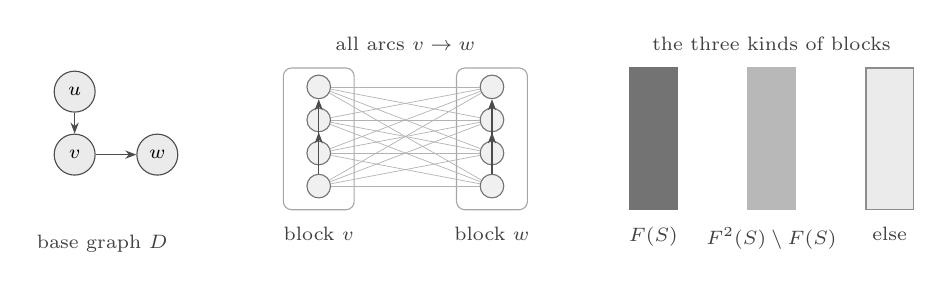
\begin{tikzpicture}[
  base/.style={circle,draw=black!70,fill=black!8,inner sep=0pt,minimum size=5.2mm,font=\scriptsize},
  labd/.style={circle,draw=black!55,fill=black!6,inner sep=0pt,minimum size=3mm},
  arc/.style={-{Stealth[length=1.4mm]},draw=black!70},
  thin/.style={draw=black!30,line width=0.25pt},
  lab/.style={font=\scriptsize,text=black!75},
  pan/.style={font=\scriptsize\bfseries,text=black!55}
]
% ---------------- panel 1: the base graph
\node[base] (u) at (0.7,2.05) {$u$};
\node[base] (v) at (0.7,1.25) {$v$};
\node[base] (w) at (1.75,1.25) {$w$};
\draw[arc] (u) -- (v);
\draw[arc] (v) -- (w);
\node[lab,anchor=north] at (1.05,0.35) {base graph $D$};
% ---------------- panel 2: the blowup of one arc
\draw[rounded corners=3pt,draw=black!35] (3.35,0.55) rectangle (4.25,2.35);
\draw[rounded corners=3pt,draw=black!35] (5.55,0.55) rectangle (6.45,2.35);
\foreach \i in {0,1,2,3}{
  \node[labd] (a\i) at (3.8,0.85+\i*0.42) {};
  \node[labd] (b\i) at (6.0,0.85+\i*0.42) {};
}
\draw[arc] (a0) -- (a3); \draw[arc] (a1) -- (a2);
\draw[arc] (b0) -- (b3); \draw[arc] (b1) -- (b2);
\foreach \i in {0,1,2,3}{ \foreach \j in {0,1,2,3}{ \draw[thin] (a\i) -- (b\j); }}
\node[lab,anchor=north] at (3.8,0.45) {block $v$};
\node[lab,anchor=north] at (6.0,0.45) {block $w$};
\node[lab,anchor=south] at (4.9,2.45) {all arcs $v\to w$};
% ---------------- panel 3: the three kinds of blocks
\draw[fill=black!55,draw=black!55] (7.75,0.55) rectangle (8.35,2.35);
\draw[fill=black!28,draw=black!28] (9.25,0.55) rectangle (9.85,2.35);
\draw[fill=black!8,draw=black!45] (10.75,0.55) rectangle (11.35,2.35);
\node[lab,anchor=north] at (8.05,0.45) {$F(S)$};
\node[lab,anchor=north] at (9.55,0.45) {$F^2(S)\setminus F(S)$};
\node[lab,anchor=north] at (11.05,0.45) {else};
\node[lab,anchor=south] at (9.55,2.45) {the three kinds of blocks};

\end{tikzpicture}

\caption{The blowup $G=D[T_m]$. \emph{Left:} the base graph $D$; a vertex $v$ and an arc $v\to w$.
 \emph{Middle:} each vertex is replaced by a transitive tournament on $m$ labels $1<\dots<m$; the arc
 $v\to w$ becomes a complete set of arcs from block $v$ to block $w$. \emph{Right:} for a set $U$
 meeting the blocks in $S$, the blocks of $F(S)$ are \emph{full} in $F_G(U)$ (dark) and the blocks of
 $F^2(S)\setminus F(S)$ are full in $F_G^2(U)$ (medium); in the remaining blocks only the internal
 image $\tau(T_v)$ is seen. \emph{Why it matters:} the full blocks contribute a multiple of $m$,
 which is where the amplification comes from; the partial blocks contribute at most $n$, which is
 the rounding error.}
\label{fig:blowup}
\end{figure}

\begin{remark}[Reading \eqref{eq:blowup-main}]\label{rem:blowup-read}
The single line \eqref{eq:blowup-main} is the whole point of the blowup, and it is worth seeing why
it is exactly what \cref{eq:deficit} says. The parenthesis
$\abs W-2\abs{F(S)}+\abs{S\cap F(S)}$ counts the blocks as follows: each block of
$F^2(S)\setminus F(S)$ contributes $+1$ (it is full in the second image but not in the first), each
block of $F(S)\setminus S$ contributes $-1$ (it is full in the first image and not in $S$), blocks
of $S\cap F(S)$ contribute $0$ (full in the first image and already in $U$), and all other blocks
contribute $0$ (they are in neither full set). So the parenthesis is precisely
$\abs{F^2(S)\setminus F(S)}-\abs{F(S)\setminus S}$: the deficit of \cref{lem:deficit}, block by
block. The factor $m$ is the number of vertices in a full block, and $\abs{S\setminus F(S)}\le n$
is the price of the blocks that are only partly seen.
\end{remark}

\begin{checkpoint}
Two sentences summarise the section. \emph{Minimality plus arc deletion} produces, for every proper
nonempty $S$, a strict deficit $\abs{F^2(S)\setminus F(S)}<\abs{F(S)\setminus S}$
(\cref{lem:deficit}); the deletion pays for the second-image gain out of the first-image loss, which
is why the deficit is strict. \emph{Blowing up} multiplies that deficit by the block size $m$ and
adds an error of at most $n$, so $m>n$ makes the sum strictly negative
(\cref{lem:blowup}). The next section builds the tool that will convert such inequalities into a
contradiction.
\end{checkpoint}

\section{Pruning two families of pairs}\label{sec:pruning}

\begin{contract}
\textbf{Assumes:} a finite set $X$ with a binary relation $\to$, and two families
$\mathcal L,\mathcal R\subseteq X\times X$ of ordered pairs, each regarded as a separate copy.
\quad
\textbf{Produces:} subfamilies $\mathcal L'\subseteq\mathcal L$ and $\mathcal R'\subseteq\mathcal R$
that do not conflict, retain every member that did not conflict to begin with, and lose at most
\[
 \abs H+\abs{\{z\in Z:\ z\text{ is covered by no member of }\mathcal L'\cup\mathcal R'\}}
\]
members, where $Z$ is the set of conflict points and $H$ the set of collisions
(\cref{def:conflict}). \quad
\textbf{Why:} \cref{sec:incompatibility} produces two families that are almost compatible and
worth more than a target value; this lemma makes them compatible at a price that the points left
uncovered pay for. Nothing here uses that $\to$ comes from an oriented graph, and nothing depends
on \cref{sec:reduction}.

\textbf{How it is proved.} In three pieces, which can be read independently.
\begin{enumerate}[label=(\alph*),leftmargin=1.5em,itemsep=1pt,topsep=1pt]
\item \emph{A cover suffices} (\cref{lem:pruning}, second half): a vertex cover of an auxiliary
  bipartite graph $\Gamma$, of size $\abs Z+\abs H$, gives the bound; the number of deletions is
  then the number of members in the cover.
\item \emph{A matching bounds the cover} (\cref{thm:konig}, proved in \appref{app:toolkit}): K\H{o}nig's
  theorem turns a bound on the maximum matching of $\Gamma$ into a cover of the same size, so it
  remains to prove $\nu(\Gamma)\le\abs Z+\abs H$.
\item \emph{The matching bound} (\cref{lem:matching}): this is the only step that uses linear
  algebra. Its proof is the longest in the paper and is the paper's second engine.
\end{enumerate}
\end{contract}

\subsection{What the lemma says}\label{sec:pruning-statement}

The objects are \emph{families of ordered pairs}. A family $\mathcal L\subseteq X\times X$ should be
pictured as a set of cells of the grid $X\times X$; a member $(p,j)$ sits in column $j$ and row $p$.
The one operation we need is \emph{advancing a coordinate along the relation}:
\begin{equation}\label{eq:Phi}
 \Phi_1 S=\{(i,j):(p,j)\in S,\ p\to i\},\qquad
 \Phi_2 S=\{(i,j):(i,s)\in S,\ s\to j\}.
\end{equation}
So $\Phi_1$ replaces the first coordinate by an out-neighbor, $\Phi_2$ the second.
\Cref{fig:conflict} shows the single most important configuration.

\begin{figure}[t]
\centering
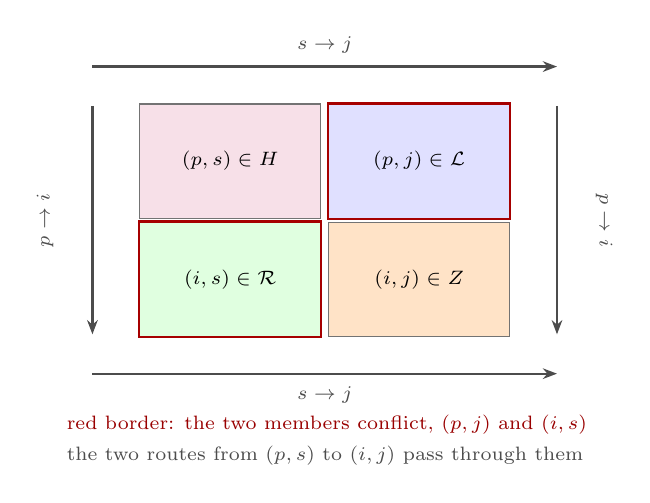
\begin{tikzpicture}[
  cell/.style={draw=black!55,minimum width=2.3cm,minimum height=1.45cm,align=center,
               font=\scriptsize,inner sep=2pt},
  hcell/.style={cell,fill=purple!12},
  lcell/.style={cell,fill=blue!12},
  rcell/.style={cell,fill=green!12},
  zcell/.style={cell,fill=orange!22},
  trav/.style={-{Stealth[length=1.8mm]},draw=black!70,thick},
  lab/.style={font=\scriptsize,text=black!70}
]
% the four cells: row p (top), row i (bottom); column s (left), column j (right)
\node[hcell] (ps) at (-1.2,0.75) {$(p,s)\in H$};
\node[lcell] (pj) at (1.2,0.75) {$(p,j)\in\mathcal L$};
\node[rcell] (is) at (-1.2,-0.75) {$(i,s)\in\mathcal R$};
\node[zcell] (ij) at (1.2,-0.75) {$(i,j)\in Z$};
% the conflicting pair: thick red border
\draw[red!65!black,thick] (pj.north west) rectangle (pj.south east);
\draw[red!65!black,thick] (is.north west) rectangle (is.south east);
% the square of traversals, outside the block
\draw[trav] (-2.95,1.45) -- (-2.95,-1.45);
\node[lab,rotate=90] at (-3.55,0) {$p\to i$};
\draw[trav] (-2.95,1.95) -- (2.95,1.95) node[midway,above=1pt,lab] {$s\to j$};
\draw[trav] (2.95,1.45) -- (2.95,-1.45);
\node[lab,rotate=-90] at (3.55,0) {$p\to i$};
\draw[trav] (-2.95,-1.95) -- (2.95,-1.95) node[midway,below=1pt,lab] {$s\to j$};
% legend
\node[lab,text=red!60!black,anchor=north west,align=left] at (-3.4,-2.35)
  {red border: the two members conflict, $(p,j)$ and $(i,s)$};
\node[lab,anchor=north west,align=left] at (-3.4,-2.75)
  {the two routes from $(p,s)$ to $(i,j)$ pass through them};
\end{tikzpicture}

\caption{A conflict, drawn as a rectangle of the grid $X\times X$. \emph{Look at} the middle column:
 the rectangle has corners $(p,s)$, $(p,j)$, $(i,s)$, $(i,j)$, and the two solid arrows are the two
 arrows of the relation that make the two members conflict. \emph{Why it matters:} the top-left cell
 $(p,s)$ is a \emph{collision} (an element of $H$) and the bottom-right cell $(i,j)$ is a
 \emph{conflict point} (an element of $Z$); a conflict is the same thing as such a rectangle, which
 is why $H$ and $Z$ are the right quantities to count. Many different conflicts can share one
 collision, and that is the reason the pruning bound cannot be proved by counting conflicts.}
\label{fig:conflict}
\end{figure}

\begin{definition}[Conflict, conflict point, collision, covering]\label{def:conflict}
Let $\mathcal L,\mathcal R\subseteq X\times X$, regarded as \emph{separate} copies of $X\times X$:
an element may belong to both, and when it does it counts twice.
\begin{itemize}[leftmargin=1.4em,itemsep=1pt,topsep=1pt]
\item $(p,j)\in\mathcal L$ and $(i,s)\in\mathcal R$ \emph{conflict} if $p\to i$ and $s\to j$.
\item $Z=\{(i,j):$ some $(p,j)\in\mathcal L$ conflicts with some $(i,s)\in\mathcal R\}$ is the set of
  \emph{conflict points}.
\item $H=\{(p,s):$ some $(p,j)\in\mathcal L$ conflicts with some $(i,s)\in\mathcal R\}$ is the set of
  \emph{collisions}.
\item A point $(i,j)\in X\times X$ is \emph{covered by} a member $(p,j)\in\mathcal L$ when $p\to i$,
  and \emph{covered by} a member $(i,s)\in\mathcal R$ when $s\to j$. These are the only ways in which
  a member covers a point: a member covers only points with which it shares a coordinate, and the
  other coordinate is advanced along the relation.
\end{itemize}
Two families are \emph{compatible} if no member of one conflicts with a member of the other.
\end{definition}

\begin{remark}[Two names, and a warning about one of them]\label{rem:names}
The points of $Z$ deserve their name: they are the points where the two images meet. The points of
$H$ do not, and the word we use for them --- \emph{collisions} --- is a historical accident of this
document: the two images of a conflict collide at $z=(i,j)$, not at $h=(p,s)$.  The right mental
picture for $h$ is the \emph{opposite corner} of the conflict rectangle in \cref{fig:conflict}.  The
distinction matters, because the whole pruning bound uses $Z$ for the points that are covered and $H$
for the corners that are not; a reader who conflates them will write a false statement, and one of us
did, in the first version of the Lean companion (see \appref{app:checks}).
\end{remark}

\begin{remark}[Compatibility is disjointness of the images]\label{rem:compat}
With $\Phi_1,\Phi_2$ as in \eqref{eq:Phi}, $\mathcal L$ and $\mathcal R$ are compatible exactly when
$\Phi_1\mathcal L\cap\Phi_2\mathcal R=\varnothing$. Indeed $(i,j)$ lies in both images exactly when
there are $(p,j)\in\mathcal L$ and $(i,s)\in\mathcal R$ with $p\to i$ and $s\to j$, which is a
conflict. Also $Z=\Phi_1\mathcal L\cap\Phi_2\mathcal R$: the set of covered points is exactly the union
of the two images, and the points of $Z$ are the ones covered from both sides.
\end{remark}

\begin{lemma}[Pruning]\label{lem:pruning}
Let $X$ be a finite set with a binary relation $\to$, and let
$\mathcal L,\mathcal R\subseteq X\times X$ be two families as in \cref{def:conflict}. Then there are
subfamilies $\mathcal L'\subseteq\mathcal L$ and $\mathcal R'\subseteq\mathcal R$ with no conflicts
between them, containing every member that is initially conflict-free, and such that
\begin{equation}\label{eq:pruning-bound}
 \abs{\mathcal L\setminus\mathcal L'}+\abs{\mathcal R\setminus\mathcal R'}
 \le\abs H+\abs{\{z\in Z:\ z\text{ is covered by no member of }\mathcal L'\cup\mathcal R'\}} .
\end{equation}
\end{lemma}

\inwords{Two families that are almost compatible can be made compatible by deleting a few members,
and the number deleted is at most the number of collisions plus the number of conflict points that
remain uncovered afterwards.}

\usedin{Applied once, in \cref{sec:incompatibility}, to the complement families
$\mathcal L=(X\times X)\setminus\Phi_2^2Q$ and $\mathcal R=(X\times X)\setminus\Phi_1^2P$. There
$H$ lies in the uncovered set of the extremal pair and the last term is at most $u'$, so the total
cost is at most $u+u'$}

\begin{ideabox}[title={Why this is the right statement}]
Three features of \eqref{eq:pruning-bound} are deliberate.
\begin{enumerate}[leftmargin=1.3em,itemsep=2pt,topsep=1pt]
\item \textbf{Only conflicts are repaired.} Members that never conflicted are kept, even if they
  cover conflict points. This is what allows the diagonal to survive in
  \cref{sec:incompatibility}: the diagonal members are conflict-free there.
\item \textbf{The cost is charged twice.} Each conflict contributes a collision (a point of $H$),
  so conflicts are counted by $H$; but different conflicts may share a collision, and a cover does
  not need to pay per conflict, only per collision. This is the first, fixed part of the cost.
\item \textbf{The remainder is charged to the survivors.} If a conflict point $z\in Z$ is still
  covered after the pruning, then some surviving member covers it, and that member occupies a vertex
  of the cover. So the number of conflict points that must be paid for individually is
  $\abs Z-q$, where $q$ is the number left uncovered. The bound is thus
  $\abs{\mathcal L\setminus\mathcal L'}+\abs{\mathcal R\setminus\mathcal R'}\le\abs H+q$, which is
  \eqref{eq:pruning-bound} rearranged. Charging part of the cost to the points still uncovered is
  exactly what the extremal argument of \cref{sec:incompatibility} needs: it can refund that part.
\end{enumerate}
\end{ideabox}


\inwords{Two families that are almost compatible can be made compatible by deleting a few members,
and the number deleted is at most the number of collisions plus the number of conflict points that
remain uncovered afterwards.}

\usedin{Applied once, in \cref{sec:incompatibility}, to the complement families
$\mathcal L=(X\times X)\setminus\Phi_2^2Q$ and $\mathcal R=(X\times X)\setminus\Phi_1^2P$. There
$H$ lies in the uncovered set of the extremal pair and the last term is at most $u'$, so the total
cost is at most $u+u'$}

\begin{example}[The bound is not the minimum number of deletions]\label{ex:k22}
Let $X=\{0,1,2\}$ and let $0\to1$, $0\to2$ be the only arrows. Take
\[
 \mathcal L=\{(0,1),(0,2)\},\qquad \mathcal R=\{(1,0),(2,0)\}.
\]
A left member $(0,j)$ and a right member $(i,0)$ conflict exactly when $0\to i$ and $0\to j$, which
here holds for all four pairs. So
\[
 Z=\{1,2\}\times\{1,2\},\qquad H=\{(0,0)\},\qquad \abs Z=4,\ \abs H=1 .
\]
Deleting one whole family costs $2$ deletions and removes all conflicts, but the survivors then
cover every point of $Z$, so the right-hand side of \eqref{eq:pruning-bound} is $\abs H+0=1$ and the
bound \emph{fails}. Keeping only $(0,1)$ costs $3$ deletions; the survivor covers $(1,1)$ and
$(2,1)$, so $q=2$ and $3=\abs H+q$. Thus no pruning with two deletions satisfies the bound, and
some pruning with three does. The lemma promises \emph{a} pruning, not the cheapest one --- a
minimum cover of the conflict graph is not enough, which is exactly why the auxiliary graph
$\Gamma$ of \cref{sec:matching} has two extra copies of every point of $Z$.
\end{example}

\begin{remark}[Why this is the right statement]\label{rem:why-pruning}
Three features of \eqref{eq:pruning-bound} are deliberate.
\begin{enumerate}[leftmargin=1.3em,itemsep=2pt,topsep=1pt]
\item \textbf{Only conflicts are repaired.} Members that never conflicted are kept, even if they
 cover conflict points. This is what allows the diagonal to survive in
 \cref{sec:incompatibility}: the diagonal members are conflict-free there.
\item \textbf{The cost is charged twice.} Each conflict contributes a collision, so conflicts are
 counted by $H$; but different conflicts may share a collision (\cref{fig:conflict}), and a cover
 does not need to pay per conflict, only per collision. This is the fixed part of the cost.
\item \textbf{The remainder is charged to the survivors.} If a conflict point $z\in Z$ is still
 covered after the pruning, some surviving member covers it, and that member occupies a vertex of
 the cover. So the number of conflict points paid for individually is $\abs Z-q$, where $q$ is the
 number left uncovered, and the bound reads
 $\abs{\mathcal L\setminus\mathcal L'}+\abs{\mathcal R\setminus\mathcal R'}\le\abs H+q$. Charging
 part of the cost to the points still uncovered is exactly what the extremal argument of
 \cref{sec:incompatibility} needs: it can refund that part.
\end{enumerate}
\end{remark}

\subsection{The rank lemma}\label{sec:kernel}

The matching bound is proved by linear algebra. The only ingredient it needs is the following
observation: at a matrix of maximum rank on a given support, a kernel vector of the matrix and a
kernel vector of its transpose cannot both be nonzero at the two ends of an allowed entry.

\begin{lemma}[Kernels at maximum support rank]\label{lem:kernel}
Let $T\subseteq I\times J$ with $I,J$ finite, and let $D\colon\R^J\to\R^I$ be a real matrix of
\emph{maximum rank among all matrices supported on $T$}, i.e.\ whose entries outside $T$ vanish.
Then for every $x\in\ker D$, every $y\in\ker D^{\mathsf T}$ and every $(s,j)\in T$,
\[
 x_j\,y_s=0 .
\]
\end{lemma}

\inwords{At a maximum-rank matrix, a vector killed by the matrix and a vector killed by its transpose
cannot both be nonzero at the two ends of an allowed entry.}

\begin{proof}
Suppose $x_jy_s\ne0$ with $(s,j)\in T$. Let $D_\tau=D+\tau e_se_j^{\mathsf T}$ for a real $\tau$;
since $(s,j)\in T$, the matrix $D_\tau$ is still supported on $T$. Because $x\in\ker D$,
\[
 D_\tau x=\tau x_j e_s ,
\]
so $e_s\in\im D_\tau$ (as $x_j\ne0$). For every $w\in\R^J$,
\[
 Dw=D_\tau w-\tau w_j e_s\in\im D_\tau ,
\]
so $\im D\subseteq\im D_\tau$. On the other hand $y$ annihilates $\im D$ (that is what
$y\in\ker D^{\mathsf T}$ means) and $y_s\ne0$, so $e_s\notin\im D$. Hence
$\im D\subsetneq\im D_\tau$ and $\rank D_\tau>\rank D$, contradicting maximality.
\end{proof}

\begin{remark}[What the lemma is for]\label{rem:kernel-use}
The lemma is applied to the auxiliary matrices $D^{p,i}$ introduced in Step~5 of the matching
bound (\cref{sec:matching}), whose rows are indexed by the right members above $i$ and whose columns
by the left members above $j$, and it is used in Step~7 to prove \eqref{eq:key}. The hypothesis that
the rank is \emph{maximum on the support} is essential and is the reason for the extra family of rank
conditions in Step~5: at a rank below the maximum, two kernel vectors could both be nonzero at an
allowed entry.
\end{remark}


\subsection{The matching bound}\label{sec:matching}

Throughout, fix the two families and let $Z,H$ be as in \cref{def:conflict}. Form the
bipartite graph $\Gamma$ with parts
\begin{equation}\label{eq:Gamma}
 \mathcal V_L=\mathcal L\sqcup Z_L,\qquad \mathcal V_R=\mathcal R\sqcup Z_R,
\end{equation}
where $Z_L$ and $Z_R$ are two disjoint copies of $Z$, also disjoint from $\mathcal L$ and
$\mathcal R$. Join two original members when they conflict; join an original member to the opposite
copy of every point of $Z$ that it covers; put no edge between $Z_L$ and $Z_R$.
\Cref{fig:pruning-graph} shows one conflict's forced path.

\begin{figure}[t]
\centering
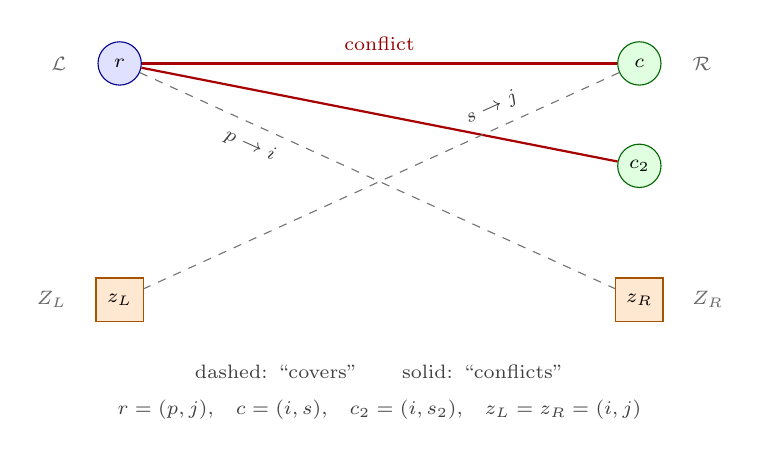
\begin{tikzpicture}[
  lv/.style={circle,draw=blue!55!black,fill=blue!12,minimum size=5.5mm,inner sep=0pt,font=\scriptsize},
  rv/.style={circle,draw=green!40!black,fill=green!12,minimum size=5.5mm,inner sep=0pt,font=\scriptsize},
  zv/.style={rectangle,draw=orange!65!black,fill=orange!18,minimum width=6mm,minimum height=5.5mm,inner sep=1pt,font=\scriptsize},
  conf/.style={draw=red!65!black,thick},
  cov/.style={draw=black!55,dashed},
  lab/.style={font=\scriptsize,text=black!75},
  grp/.style={font=\scriptsize\bfseries,text=black!60}
]
\node[lv] (r) at (0,3.2) {$r$};
\node[zv] (zl) at (0,0.2) {$z_L$};
\node[rv] (c) at (6.6,3.2) {$c$};
\node[rv] (c2) at (6.6,1.9) {$c_2$};
\node[zv] (zr) at (6.6,0.2) {$z_R$};
\node[grp,anchor=east] at (-0.55,3.2) {$\mathcal L$};
\node[grp,anchor=east] at (-0.55,0.2) {$Z_L$};
\node[grp,anchor=west] at (7.15,3.2) {$\mathcal R$};
\node[grp,anchor=west] at (7.15,0.2) {$Z_R$};
\draw[conf] (r) -- node[above=1pt,lab,text=red!60!black] {conflict} (c);
\draw[conf] (r) -- (c2);
\draw[cov] (c) -- node[near start,above=1pt,lab,sloped] {$s\to j$} (zl);
\draw[cov] (r) -- node[near start,below=1pt,lab,sloped] {$p\to i$} (zr);
\node[lab,anchor=north] at (3.3,-0.5) {dashed: ``covers''\qquad solid: ``conflicts''};
\node[lab,anchor=north] at (3.3,-0.95) {$r=(p,j)$,\quad $c=(i,s)$,\quad $c_2=(i,s_2)$,\quad $z_L=z_R=(i,j)$};
\end{tikzpicture}

\caption{The augmented bipartite graph $\Gamma$. \emph{Look at} the path
 $z_L-c-r-z_R$ forced by the conflict between $r=(p,j)\in\mathcal L$ and $c=(i,s)\in\mathcal R$,
 where $z=(i,j)$: the two dashed edges are the covering relations $s\to j$ and $p\to i$, the solid
 edges are conflicts. \emph{Why it matters:} conflicts and covering relations become edges of one
 bipartite graph, so that a single vertex cover pays for both: a conflict edge forces ``delete $r$ or
 delete $c$'', while a covering edge forces ``delete the member or spend the copy of $z$''. The
 second conflict drawn shares $r$, showing that the graph is not a disjoint union of such paths ---
 which is why a matching bound, not a path count, is needed.}
\label{fig:pruning-graph}
\end{figure}

\begin{lemma}[Matching bound]\label{lem:matching}
The maximum size $\nu(\Gamma)$ of a matching in $\Gamma$ satisfies
\[
 \nu(\Gamma)\le \abs Z+\abs H .
\]
\end{lemma}

\inwords{A maximum matching of the augmented graph has at most as many edges as there are conflict
points plus collisions.}

\begin{planbox}
\begin{enumerate}[leftmargin=1.3em,itemsep=1pt,topsep=1pt]
\item \textbf{Split the matching} (Step~2): choose a maximum matching $\mathcal M$ minimizing the
 number $k$ of original--original edges. Its other edges come in two families, $\alpha$ of size
 $\ell$ and $\beta$ of size $t$, and each of $\alpha,\beta$ is a maximum matching in its own
 subgraph.
\item \textbf{Encode by ranks} (Steps 3--5): build four matrices $L,N,A,B$ forming a commutative
 square $NL=AB$, and choose the coefficients so that $\rank L=\ell$, $\rank N^{\mathsf T}=t$ and
 some auxiliary matrices have maximum rank on their supports.
\item \textbf{Rank bookkeeping} (Step~4, used later): rank--nullity and the square give
 $\abs H\ge k+\ell+t-\abs Z$ as soon as $\dim\ker A\ge k$.
\item \textbf{Feed the kernel} (Steps 6--7): lift the $k$ original left endpoints to vectors
 $\lambda^r\in\ker L$ and show that their images $B\lambda^r$ are independent, using the rank lemma
 at the conflicting pairs.
\end{enumerate}
\end{planbox}

\begin{proof}
\steplabel{Step 1: the graph.}\label{step:gamma}
Throughout, $\Gamma$ is the augmented bipartite graph of \eqref{eq:Gamma}: its vertices are the
members of $\mathcal L$ and $\mathcal R$ together with the two copies $Z_L,Z_R$ of the conflict
points, and its edges are the conflicts and the covering relations. We must show that a matching of
$\Gamma$ has at most $\abs Z+\abs H$ edges.

\steplabel{Step 2: a maximum matching, split in three.}
Choose a maximum matching $\mathcal M$ of $\Gamma$ with as few edges as possible between two original
members. Write $k$ for the number of those edges, and let
\begin{equation}\label{eq:alpha-beta}
 \alpha=\mathcal M\cap(\mathcal L\times Z_R),\qquad
 \beta=\mathcal M\cap(Z_L\times\mathcal R),\qquad
 \ell=\abs\alpha,\qquad t=\abs\beta,
\end{equation}
so that $\abs{\mathcal M}=k+\ell+t$: these are the only kinds of edges of $\Gamma$.

\emph{$\alpha$ is a maximum matching between $\mathcal L$ and $Z_R$.} Suppose that subgraph had a
larger matching. Its symmetric difference with $\alpha$ contains an $\alpha$-augmenting path $P$
from an $\alpha$-unmatched member $r\in\mathcal L$ to an $\alpha$-unmatched vertex $z\in Z_R$. Every
internal vertex of $P$ is matched by $\alpha$, and $z$ is unmatched in $\mathcal M$ altogether
(because $z\in Z_R$ has neighbors only in $\mathcal L$, where $\mathcal M$ acts through $\alpha$).
If $r$ is unmatched in $\mathcal M$, augmenting along $P$ enlarges $\mathcal M$, which is impossible.
If $r$ is matched in $\mathcal M$, it is matched by an original--original edge (it is unmatched by
$\alpha$), and removing that edge and augmenting along $P$ keeps the size of $\mathcal M$ and lowers
$k$, contradicting the choice of $\mathcal M$. So no larger matching exists. The same argument with
the sides exchanged shows that $\beta$ is a maximum matching between $Z_L$ and $\mathcal R$. Write
$R_\alpha\subseteq\mathcal L$ and $C_\beta\subseteq\mathcal R$ for the original vertices matched by
$\alpha$ and by $\beta$.

\steplabel{Step 3: four matrices and the commutative square.}
For every arrow $x\to y$ of the relation introduce two \emph{independent} real variables
$a_{xy}$ and $b_{xy}$, and set an entry to $0$ whenever the corresponding arrow is absent. For any
assignment of the variables define four matrices
\begin{equation}\label{eq:fourmaps}
 \begin{array}{ccc}
 \R^{\mathcal L}&\xrightarrow{\ L\ }&\R^{Z}\\[2pt]
 {\scriptstyle B}\big\downarrow&&\big\downarrow{\scriptstyle N}\\[2pt]
 \R^{H}&\xrightarrow{\ A\ }&\R^{\mathcal R}
 \end{array}
 \qquad
 \begin{aligned}
  L_{(i,j),(p,j)}&=a_{pi},&\quad N_{(i,s),(i,j)}&=b_{sj},\\
  B_{(p,s),(p,j)}&=b_{sj},&\quad A_{(i,s),(p,s)}&=a_{pi},
 \end{aligned}
\end{equation}
all other entries being zero; the indices range over the indicated coordinate sets, so for instance
$L_{(i,j),(p,j)}$ is defined only for $(i,j)\in Z$ and $(p,j)\in\mathcal L$. The maps $L$ and $A$
advance the \emph{first} coordinate along an arrow $p\to i$; the maps $N$ and $B$ advance the
\emph{second} coordinate along an arrow $s\to j$. Two steps can be composed in two orders, and
\Cref{fig:fourmaps} shows that the two orders give the same result:
\begin{equation}\label{eq:commute}
 NL=AB .
\end{equation}
Indeed, the entry of $NL$ at $((i,s),(p,j))$ is $a_{pi}b_{sj}$ if $(i,j)\in Z$ and $0$ otherwise,
while the entry of $AB$ at the same place is $a_{pi}b_{sj}$ if $(p,s)\in H$ and $0$ otherwise. For
$(p,j)\in\mathcal L$ and $(i,s)\in\mathcal R$ the two conditions are equivalent: either both hold,
when the two members conflict, or neither does, and then $a_{pi}b_{sj}=0$ because at least one of
the two arrows is missing.

\begin{figure}[t]
\centering
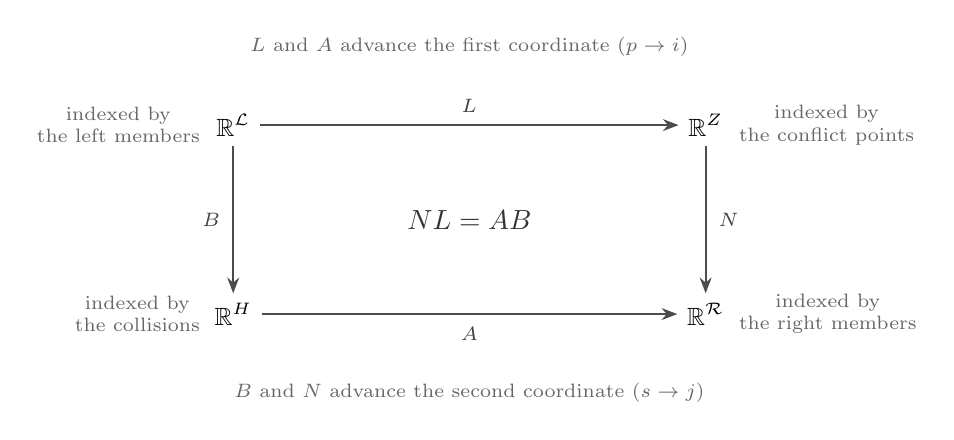
\begin{tikzpicture}[
  sp/.style={font=\small},
  ar/.style={-{Stealth[length=2mm]},draw=black!70,thick},
  lab/.style={font=\scriptsize,text=black!75},
  note/.style={font=\scriptsize,text=black!60,align=center}
]
\node[sp] (L) at (0,2.4) {$\R^{\mathcal L}$};
\node[sp] (Z) at (6.0,2.4) {$\R^{Z}$};
\node[sp] (H) at (0,0) {$\R^{H}$};
\node[sp] (R) at (6.0,0) {$\R^{\mathcal R}$};
\draw[ar] (L) -- node[above=1pt,lab] {$L$} (Z);
\draw[ar] (L) -- node[left=1pt,lab] {$B$} (H);
\draw[ar] (H) -- node[below=1pt,lab] {$A$} (R);
\draw[ar] (Z) -- node[right=1pt,lab] {$N$} (R);
\node[lab,text=black!80,font=\normalsize] at (3.0,1.2) {$NL=AB$};
\node[note,anchor=east] at (-0.3,2.4) {indexed by\\ the left members};
\node[note,anchor=west] at (6.3,2.4) {indexed by\\ the conflict points};
\node[note,anchor=east] at (-0.3,0) {indexed by\\ the collisions};
\node[note,anchor=west] at (6.3,0) {indexed by\\ the right members};
\node[note,anchor=south] at (3.0,3.15) {$L$ and $A$ advance the first coordinate ($p\to i$)};
\node[note,anchor=north] at (3.0,-0.75) {$B$ and $N$ advance the second coordinate ($s\to j$)};
\end{tikzpicture}

\caption{The commutative square \eqref{eq:commute}. \emph{Look at} the two routes from
 $\R^{\mathcal L}$ to $\R^{\mathcal R}$: one goes through $\R^{Z}$, the other through $\R^{H}$, and
 the two composites agree. \emph{Why it matters:} this is the same square as the grid picture of
 \cref{fig:conflict} --- advancing the first coordinate and then the second, or the other way round,
 both take a left member to a right member, with intermediate cells $(i,j)\in Z$ and
 $(p,s)\in H$ --- and \eqref{eq:commute} is the only link between the matching $\mathcal M$ (whose
 pieces are counted by $Z$ and $H$) and the kernel of $A$ (which is where the $k$
 original--original edges are hidden).}
\label{fig:fourmaps}
\end{figure}

\steplabel{Step 4: rank bookkeeping.}
Suppose the coefficients are chosen so that
\begin{equation}\label{eq:rank-conditions}
 \rank L=\ell,\qquad \rank N^{\mathsf T}=t,\qquad \dim\ker A\ge k .
\end{equation}
Then, writing $\dim\ker A=\abs H-\rank A$ by rank--nullity,
\begin{align}
 \abs H&=\dim\ker A+\rank A\ge k+\rank A\ge k+\rank(NL)\notag\\
 &\ge k+\bigl(\ell-(\abs Z-t)\bigr)=k+\ell+t-\abs Z ,
 \label{eq:rank-bound}
\end{align}
where the second inequality uses $\im(NL)\subseteq\im A$ (from $NL=AB$) and the third restricts $N$
to $\im L$:
\begin{equation}\label{eq:rank-restrict}
 \rank(NL)=\dim\im L-\dim(\im L\cap\ker N)\ge\ell-(\abs Z-t),
\end{equation}
since $\dim\im L=\rank L=\ell$ and $\im L\cap\ker N\subseteq\ker N$ with
$\dim\ker N=\abs Z-\rank N=\abs Z-t$. Hence $\abs{\mathcal M}=k+\ell+t\le\abs Z+\abs H$, which is
the matching bound we need.

The first two conditions of \eqref{eq:rank-conditions} will come from $\alpha$ and $\beta$. The third
is the subtle one: it will be produced from the $k$ original--original edges, by finding $k$
independent vectors in $\ker A$.

\steplabel{Step 5: choosing the coefficients.}
We must justify that \eqref{eq:rank-conditions} can hold, together with one further family of rank
conditions, all at the same assignment. Two facts about ranks and matchings do all the work, and both
are proved in \appref{app:toolkit}:
\begin{itemize}[leftmargin=1.4em,itemsep=1pt,topsep=1pt]
\item \emph{a nonzero minor exhibits a matching} (\cref{lem:minor-matching}): a matrix supported on a
 set $T$ has rank at most $\nu(T)$, the largest number of entries of $T$ no two in a row or column;
\item \emph{an explicit matching gives an explicit maximal-rank matrix}: placing $1$s on the entries
 of a maximum matching and $0$s elsewhere produces a matrix of rank $\nu(T)$ supported on $T$,
 and every nonzero minor of such a matrix is a product of \emph{distinct} variables, hence a nonzero
 polynomial.
\end{itemize}
So for each of the matrices below we argue twice: an upper bound for \emph{every} assignment (no
support-matching is larger than the maximum matching we already have), and the existence of \emph{one}
assignment attaining it (an explicit minor whose determinant does not vanish identically). The
maximizing assignments of the various matrices must be combined, which is what (5d) does.

\emph{(5a) $\rank L=\ell$ with the columns $R_\alpha$ a basis of $\im L$.} For any assignment, a
nonzero $r\times r$ minor of $L$ needs $r$ entries no two in the same row or column and all nonzero,
i.e.\ a matching of size $r$ between $\mathcal L$ and $Z_R$; since $\alpha$ is maximum, $r\le\ell$ and
therefore $\rank L\le\ell$ always. For the reverse inequality consider the square minor with rows the
$Z$-endpoints of $\alpha$ and columns $R_\alpha$. Its entries $L_{(i,j),(p,j)}=a_{pi}$ vanish unless
the two second coordinates agree, so the minor is block diagonal with one block for each value of $j$.
Inside a block the only nonzero entries are the variables $a_{pi}$ of the matched pairs, one per row
and column, so the determinant is, up to sign, the product of those variables. Different permutations
of a block use different sets of variables, so no cancellation occurs: the determinant is a nonzero
polynomial in the $a$-variables. The determinant of the whole minor is the product of the block
determinants, up to sign (variables may occur in more than one block, but a product of nonzero
polynomials is nonzero). Hence at any assignment where this one polynomial does not vanish,
$\rank L=\ell$ and the columns $R_\alpha$ are independent, hence a basis of $\im L$.

\emph{(5b) $\rank N^{\mathsf T}=t$ with the columns $C_\beta$ a basis of $\im N^{\mathsf T}$.} The same
argument, with the roles of the two coordinates exchanged: the minor with rows the $Z$-endpoints of
$\beta$ and columns $C_\beta$ is block diagonal with one block per value of the \emph{first}
coordinate, each block determinant a product of distinct $b$-variables.

\emph{(5c) The auxiliary matrices.} For every arrow $p\to i$ of the relation put
\begin{equation}\label{eq:Dpi}
 J_p=\{j:(p,j)\in\mathcal L\},\qquad S_i=\{s:(i,s)\in\mathcal R\},
 \qquad D^{p,i}=(b_{sj})_{s\in S_i,\ j\in J_p} .
\end{equation}
So $D^{p,i}$ has rows indexed by $S_i$ and columns by $J_p$, and it is supported on
\begin{equation}\label{eq:Tpi}
 T^{p,i}=\{(s,j)\in S_i\times J_p:\ s\to j\}.
\end{equation}
For each arrow $p\to i$, choose a minor of $D^{p,i}$ that attains the maximum rank among matrices
supported on $T^{p,i}$; the entries of the minor are $b$-variables, so its determinant is a nonzero
polynomial in the $b$-variables, or the empty minor $1$ if that maximum rank is $0$. These matrices
are what connects the two kernels in Step~7: a conflict is exactly a triple with $(s,j)\in T^{p,i}$.

\emph{(5d) One assignment for everything.} Multiply the finitely many nonzero polynomials obtained in
(5a)--(5c). The product is a nonzero polynomial in the finitely many variables $a_{xy},b_{xy}$, since
the polynomial ring is an integral domain. A nonzero real polynomial in finitely many variables is
nonzero at some real point: induct on the number of variables, writing the polynomial as a polynomial
in the last variable whose coefficients are polynomials in the others. Fix once and for all a real
assignment at which the product does not vanish. At that assignment all the required minors are
nonzero simultaneously: $\rank L=\ell$ with $R_\alpha$ a basis of $\im L$, $\rank N^{\mathsf T}=t$
with $C_\beta$ a basis of $\im N^{\mathsf T}$, and every $D^{p,i}$ has maximum rank on $T^{p,i}$.

\steplabel{Step 6: lifting the original--original edges.}
For each original--original edge $(r,c)\in\mathcal M$, say $r=(p,j)\in\mathcal L$ and
$c=(i,s)\in\mathcal R$, the basis property of $R_\alpha$ provides coefficients $\xi^r_a$ with
\begin{equation}\label{eq:lifts}
 \lambda^r=e_r+\sum_{a\in R_\alpha}\xi^r_a\,e_a\in\ker L,
 \qquad
 \kappa^c=e_c+\sum_{b\in C_\beta}\eta^c_b\,e_b\in\ker N^{\mathsf T}.
\end{equation}
Such vectors exist because the column $Le_r$ of $L$ lies in $\im L=\Span\{Le_a:a\in R_\alpha\}$, so a
suitable linear combination of the $e_a$ cancels it. The endpoints $r$ and $c$ of an
original--original edge are matched by $\mathcal M$, hence not matched by $\alpha$ or $\beta$, so
$r\notin R_\alpha$ and $c\notin C_\beta$; consequently
\[
 \lambda^r_r=1,\qquad \lambda^r_{r'}=0\ \text{for every other original left endpoint }r',
 \qquad \kappa^c_c=1 .
\]

\steplabel{Step 7: the key vanishing, and $\dim\ker A\ge k$.}
The assertion to prove is
\begin{equation}\label{eq:key}
 u_{pj}\,v_{is}=0
 \qquad\text{for every conflict }\bigl((p,j),(i,s)\bigr),\quad
 u\in\ker B,\quad v\in\ker N^{\mathsf T}.
\end{equation}
Here $u\in\ker B\subseteq\R^{\mathcal L}$ and $v\in\ker N^{\mathsf T}\subseteq\R^{\mathcal R}$, so
the two factors are coordinates of the two vectors at the two conflicting members.

Fix an arrow $p\to i$ and $u\in\ker B$. The coordinate of $Bu=0$ at $(p,s)\in H$ reads
\begin{equation}\label{eq:row-eq}
 \sum_{j\in J_p}b_{sj}u_{pj}=0 .
\end{equation}
If a row $s\in S_i$ of $D^{p,i}$ has an allowed entry, choose $j\in J_p$ with $s\to j$; then $(p,j)$
and $(i,s)$ conflict (as $p\to i$), so $(p,s)\in H$ and \eqref{eq:row-eq} is exactly the statement
that the row $s$ of $D^{p,i}$ annihilates the vector $(u_{pj})_{j\in J_p}$. If the row has no allowed
entry, all its entries are $0$ and the same equation holds trivially. So
$(u_{pj})_{j\in J_p}\in\ker D^{p,i}$.

Similarly, for $v\in\ker N^{\mathsf T}$, the coordinate of $N^{\mathsf T}v=0$ at $(i,j)$ reads
\begin{equation}\label{eq:col-eq}
 \sum_{s\in S_i}b_{sj}v_{is}=0 ,
\end{equation}
which is the statement that $(v_{is})_{s\in S_i}$ is annihilated by the columns of $D^{p,i}$; the
coordinate $(i,j)$ is available in $Z$ whenever some $s\in S_i$ has $s\to j$, and the equation holds
trivially otherwise. So $(v_{is})_{s\in S_i}\in\ker(D^{p,i})^{\mathsf T}$.

Since $D^{p,i}$ has maximum rank on its support $T^{p,i}$, \cref{lem:kernel} applies to the two kernel
vectors and gives $u_{pj}v_{is}=0$ for every $(s,j)\in T^{p,i}$, i.e.\ whenever $s\to j$, which is
exactly \eqref{eq:key}. Note that the single-entry perturbation inside \cref{lem:kernel} is applied to
$D^{p,i}$ alone and need not preserve any other rank condition; the conclusion holds for the fixed
assignment of Step~5.

Now substitute $v=\kappa^c$ in \eqref{eq:key} for an original--original edge $(r,c)$ with $r=(p,j)$ and
$c=(i,s)$. Since $\kappa^c_c=1$, \eqref{eq:key} says $u_{pj}=0$ for every $u\in\ker B$: every vector of
$\ker B$ vanishes at $r$. Therefore the vectors $B\lambda^r$, for $r$ ranging over the $k$ original
left endpoints, are linearly independent. Indeed a relation $\sum_r\theta_rB\lambda^r=0$ puts
$u=\sum_r\theta_r\lambda^r$ in $\ker B$, and the coordinate of $u$ at each $r$ is $u_r=\theta_r$ by
\eqref{eq:lifts}; all these coordinates vanish, so all $\theta_r$ vanish. Moreover
\[
 A(B\lambda^r)=NL\lambda^r=0
\]
by \eqref{eq:commute}, because $\lambda^r\in\ker L$. So the $B\lambda^r$ are $k$ independent vectors
of $\ker A$, i.e.\ $\dim\ker A\ge k$. This is the third condition of \eqref{eq:rank-conditions}, and
Step~4 now gives $\abs{\mathcal M}\le\abs Z+\abs H$.

\end{proof}

\subsection{From the matching bound to the pruning}\label{sec:matching-to-pruning}

\begin{proof}[Proof of \cref{lem:pruning}]
If there is no conflict at all, keep every member; then $Z=H=\varnothing$ and
\eqref{eq:pruning-bound} is trivial. Otherwise build $\Gamma$ as in \eqref{eq:Gamma}.

\emph{An initially conflict-free member is isolated in $\Gamma$.} Let $(p,j)\in\mathcal L$ be
conflict-free and suppose it covers $(i,j)\in Z$. By definition of $Z$ there is a conflict between
some $(\tilde p,j)\in\mathcal L$ and some $(i,s)\in\mathcal R$; in particular $s\to j$. Then
$(p,j)$ and $(i,s)$ satisfy $p\to i$ and $s\to j$, so they conflict, contrary to the assumption.
The same argument with the sides exchanged applies to $\mathcal R$. So conflict-free members have
no edges at all.

\emph{A cover gives the bound.} By \cref{thm:konig} (proved in \appref{app:toolkit}) the graph
$\Gamma$ has a vertex cover $K$ with $\abs K=\nu(\Gamma)\le\abs Z+\abs H$ that contains exactly one
endpoint of each edge of a maximum matching and no unmatched vertices; in particular it contains no
isolated vertex. Delete exactly the original members lying in $K$. Since $K$ covers every edge, no
conflict survives, and since $K$ contains no isolated vertex, no initially conflict-free member is
deleted. Let $q$ be the number of points of $Z$ covered by no surviving member. Each of the other
$\abs Z-q$ points $z\in Z$ is covered by some surviving member; that member is adjacent to one of
the two copies of $z$, so that copy lies in $K$, because the edge between them is not covered from
the other side (the member is not in $K$). Distinct points have distinct copies, so
\begin{equation}\label{eq:cover-charge}
 \abs{K\cap(\mathcal L\sqcup\mathcal R)}
 \le\abs K-(\abs Z-q)\le\abs H+q ,
\end{equation}
which is \eqref{eq:pruning-bound}. \Cref{fig:cover} records the counting.
\end{proof}

\begin{figure}[t]
\centering
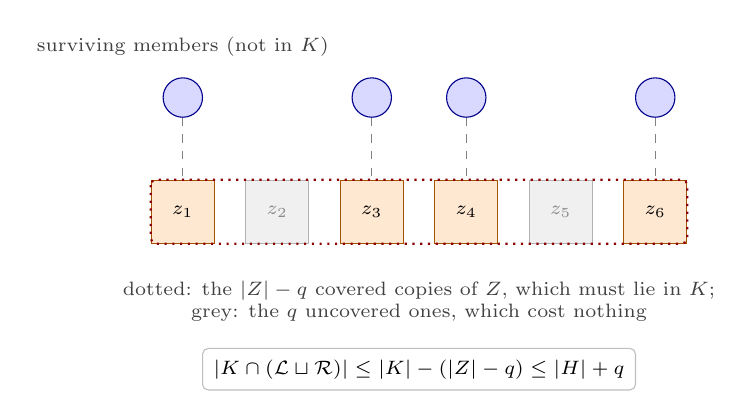
\begin{tikzpicture}[
  zv/.style={rectangle,draw=orange!65!black,fill=orange!18,minimum width=8mm,minimum height=8mm,inner sep=0pt,font=\scriptsize},
  unc/.style={rectangle,draw=black!30,fill=black!6,minimum width=8mm,minimum height=8mm,inner sep=0pt,
              font=\scriptsize,text=black!45},
  mem/.style={circle,draw=blue!55!black,fill=blue!15,minimum size=5mm,inner sep=0pt},
  cov/.style={draw=black!50,dashed},
  lab/.style={font=\scriptsize,text=black!75}
]
\node[zv]  (z1) at (0.0,0) {$z_1$};
\node[unc] (z2) at (1.2,0) {$z_2$};
\node[zv]  (z3) at (2.4,0) {$z_3$};
\node[zv]  (z4) at (3.6,0) {$z_4$};
\node[unc] (z5) at (4.8,0) {$z_5$};
\node[zv]  (z6) at (6.0,0) {$z_6$};
\node[mem] (m1) at (0.0,1.45) {};
\node[mem] (m3) at (2.4,1.45) {};
\node[mem] (m4) at (3.6,1.45) {};
\node[mem] (m6) at (6.0,1.45) {};
\foreach \a/\b in {m1/z1,m3/z3,m4/z4,m6/z6}{ \draw[cov] (\a) -- (\b); }
\draw[red!55!black,dotted,thick,rounded corners=2pt] (z1.north west) rectangle (z6.south east);
\node[lab,anchor=south] at (0.0,1.85) {surviving members (not in $K$)};
\node[lab,anchor=north,align=center] at (3.0,-0.75)
  {dotted: the $\abs Z-q$ covered copies of $Z$, which must lie in $K$;\\
   grey: the $q$ uncovered ones, which cost nothing};
\node[draw=black!25,fill=white,rounded corners=2pt,inner sep=4pt,font=\scriptsize]
  at (3.0,-2.0) {$\abs{K\cap(\mathcal L\sqcup\mathcal R)}\le\abs K-(\abs Z-q)\le\abs H+q$};
\end{tikzpicture}

\caption{The counting behind \eqref{eq:cover-charge}. \emph{Look at} the row of copies of the points
 of $Z$: the $q$ points left uncovered cost nothing, and each of the remaining $\abs Z-q$ must have a
 copy in $K$ because the edge from it to its surviving member is not covered from the other side.
 \emph{Why it matters:} this is the only place where the ``uncovered'' term of the pruning bound comes
 from, and it is why the bound degrades gracefully: the more the survivors leave uncovered, the less
 the cover has to pay for the points of $Z$.}
\label{fig:cover}
\end{figure}

\begin{checkpoint}
The lemma is proved. Three sentences to keep: \emph{conflicts and covering relations become edges of
a bipartite graph $\Gamma$}; \emph{K\"onig turns a bound on the maximum matching of $\Gamma$ into a
vertex cover of the same size, and deleting its original members is the pruning}; \emph{a maximum
matching has at most $\abs Z+\abs H$ edges, because the two coverage matchings $\alpha,\beta$ and the
$k$ original--original edges are three quantities that ranks can count, and the commuting square
$NL=AB$ forces the $k$ lifts into the kernel of $A$}. The next section applies the lemma to the
families produced by the subset inequalities of \cref{sec:reduction}.
\end{checkpoint}

\begin{remark}[What the rank argument is really doing]\label{rem:rank-philosophy}
It is worth separating the three roles of linear algebra in Steps 3--7, because the proof is easy to
read as a sequence of tricks.
\begin{enumerate}[leftmargin=1.3em,itemsep=2pt,topsep=1pt]
\item \textbf{Rank as a matching counter.} The maximum rank of a matrix supported on a set $T$ equals
  the maximum size of a matching in $T$; only the easy direction is needed
  (\cref{lem:minor-matching}): a nonzero
  minor exhibits a matching, so $\rank\le$ matching size; and the explicit minors of (5a), (5b) are
  chosen to \emph{achieve} the matching bound. Thus $\rank L=\ell$ is a certificate that
  $\alpha$ is maximum, and $\rank N^{\mathsf T}=t$ that $\beta$ is.
\item \textbf{Rank--nullity as a trade-off.} If a matrix from a space of dimension $\abs H$ has rank
  $r$, its kernel has dimension $\abs H-r$. So a lower bound on the kernel is an upper bound on the
  rank, hence on a matching. This is the chain \eqref{eq:rank-bound}: $\dim\ker A\ge k$ and
  $\rank A\ge\rank(NL)$ together give $\abs H\ge k+\ell+t-\abs Z$.
\item \textbf{The commuting square as incompatibility.} The identity $NL=AB$ says that a conflict can
  be traversed in two ways. If both a left kernel vector and a right kernel vector were nonzero at the
  two ends of a conflict, the two routes would force a contradiction, and the rank lemma turns that
  into the vanishing \eqref{eq:key}. That vanishing is what makes $k$ vectors out of nothing: the
  right kernel vector $\kappa^c$ kills the coordinate of every left kernel vector at $r$.
\end{enumerate}
\end{remark}

\section{The extremal contradiction}\label{sec:incompatibility}

\begin{contract}
\textbf{Assumes:} \cref{prop:reduction}, i.e.\ a graph $G$ with positive indegrees satisfying
$\abs U+\abs{F^2(U)}<2\abs{F(U)}$ for every nonempty proper $U$. \quad
\textbf{Produces:} a contradiction (\cref{prop:no-concavity}), hence \cref{thm:main}.
\textbf{Why:} this is where the subset inequality and the pruning lemma meet. The subset inequality
applied to the rows and columns of two families of pairs yields two \emph{better} families that may
conflict; the pruning lemma repairs the conflicts without losing the improvement.
\end{contract}

\subsection{The setting}\label{sec:setting}

For the rest of the section fix an oriented graph $G$ with vertex set $X$, all indegrees positive,
and
\begin{equation}\label{eq:hypothesis}
 \abs U+\abs{F^2(U)}<2\abs{F(U)}
 \qquad\text{for every }\varnothing\ne U\subsetneq X .
\end{equation}
The object we extremise over is a \emph{pair of families of ordered pairs}, exactly as in
\cref{sec:pruning}. The two coordinate maps of \eqref{eq:Phi} act on them:
\begin{equation}\label{eq:Phi-again}
 \Phi_1 P=\{(i,j):(p,j)\in P,\ p\to i\},\qquad
 \Phi_2 Q=\{(i,j):(i,s)\in Q,\ s\to j\},
\end{equation}
and we abbreviate $\Phi_1^2P=\Phi_1(\Phi_1P)$ and $\Phi_2^2Q=\Phi_2(\Phi_2Q)$. Two families are
\emph{compatible} if $\Phi_1P\cap\Phi_2Q=\varnothing$ (\cref{rem:compat}). \Cref{fig:grid} fixes the
picture, and $\Delta=\{(v,v):v\in X\}$ is the diagonal.

\begin{figure}[t]
\centering
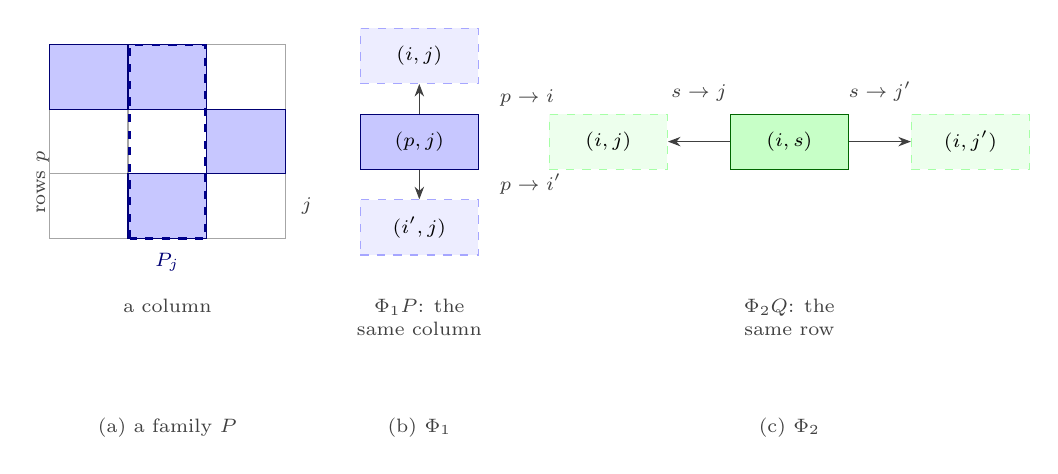
\begin{tikzpicture}[
  cell/.style={draw=black!35,minimum width=1.0cm,minimum height=0.82cm,inner sep=0pt},
  widecell/.style={draw=black!45,minimum width=1.5cm,minimum height=0.7cm,align=center,
                   font=\scriptsize,inner sep=1pt},
  filled/.style={cell,fill=blue!22,draw=blue!45!black},
  wfilled/.style={widecell,fill=blue!22,draw=blue!45!black},
  wghost/.style={widecell,fill=blue!7,draw=blue!35,dashed},
  rfilled/.style={widecell,fill=green!22,draw=green!40!black},
  rghost/.style={widecell,fill=green!7,draw=green!35,dashed},
  ar/.style={-{Stealth[length=1.6mm]},draw=black!75},
  lab/.style={font=\scriptsize,text=black!75},
  pan/.style={font=\scriptsize\bfseries,text=black!55}
]
% ---------------- (a) a family and one of its columns
\begin{scope}
\foreach \i in {0,1,2}{\foreach \j in {0,1,2}{
  \node[cell] at (\j*1.0+0.5, \i*0.82+0.41) {};}}
\node[filled] at (0.5,2.05) {};
\node[filled] at (1.5,2.05) {};
\node[filled] at (1.5,0.41) {};
\node[filled] at (2.5,1.23) {};
\draw[blue!55!black,dashed,thick] (1.02,0.0) rectangle (1.98,2.46);
\node[lab,anchor=north,text=blue!45!black] at (1.5,-0.06) {$P_j$};
\node[lab,anchor=north,align=center] at (1.5,-0.65) {a column};
\node[lab,anchor=north] at (1.5,-2.15) {(a) a family $P$};
\node[lab,anchor=east,rotate=90] at (-0.08,1.23) {rows $p$};
\node[lab,anchor=west] at (3.08,0.41) {$j$};

\end{scope}
% ---------------- (b) Phi_1 inside a column
\begin{scope}[shift={(4.7,0)}]
\node[wghost] (u) at (0,2.32) {$(i,j)$};
\node[wfilled] (c) at (0,1.23) {$(p,j)$};
\node[wghost] (d) at (0,0.14) {$(i',j)$};
\draw[ar] (c.north) -- (u.south);
\draw[ar] (c.south) -- (d.north);
\node[lab,anchor=west] at (0.9,1.78) {$p\to i$};
\node[lab,anchor=west] at (0.9,0.69) {$p\to i'$};
\node[lab,anchor=north,align=center] at (0,-0.65) {$\Phi_1P$: the\\ same column};
\node[lab,anchor=north] at (0,-2.15) {(b) $\Phi_1$};
\end{scope}
% ---------------- (c) Phi_2 inside a row
\begin{scope}[shift={(9.4,0)}]
\node[rghost] (l) at (-2.3,1.23) {$(i,j)$};
\node[rfilled] (c2) at (0,1.23) {$(i,s)$};
\node[rghost] (r2) at (2.3,1.23) {$(i,j')$};
\draw[ar] (c2.west) -- (l.east);
\draw[ar] (c2.east) -- (r2.west);
\node[lab,anchor=south] at (-1.15,1.62) {$s\to j$};
\node[lab,anchor=south] at (1.15,1.62) {$s\to j'$};
\node[lab,anchor=north,align=center] at (0,-0.65) {$\Phi_2Q$: the\\ same row};
\node[lab,anchor=north] at (0,-2.15) {(c) $\Phi_2$};
\end{scope}
\end{tikzpicture}

\caption{Families of pairs as cells of the grid $X\times X$. \emph{(a)} A family $P$; its
 \emph{columns} are the sets $P_j=\{p:(p,j)\in P\}$, one for each second coordinate (and its rows are
 defined the same way). \emph{(b)} The map $\Phi_1$ replaces the first coordinate $p$ by an
 out-neighbor $i$: it moves a cell within its column. \emph{(c)} The map $\Phi_2$ replaces the second
 coordinate $s$ by an out-neighbor $j$: it moves a cell within its row. \emph{Why it matters:} the
 hypothesis \eqref{eq:hypothesis} is a statement about \emph{sets of vertices}, so it can only be
 applied to the columns of $P$ and the rows of $Q$; summing it over those sets is what produces
 \eqref{eq:fiber-sums}.}
\label{fig:grid}
\end{figure}

\begin{proposition}\label{prop:no-concavity}
There is no nonempty finite oriented graph $G$ in which every vertex has an in-neighbor and whose
one-step image operator $F(U)=\{y: x\to y\text{ for some }x\in U\}$ satisfies
\begin{equation}\label{eq:impossible}
 \abs U+\abs{F^2(U)}<2\abs{F(U)}
 \qquad\text{for every }\varnothing\ne U\subsetneq V(G).
\end{equation}
\end{proposition}

\inwords{No graph satisfies the strict subset inequality at every proper nonempty set once every
vertex has an in-neighbor.}

\begin{ideabox}[title={The design of the extremal objective}]
We look for a compatible pair $(P,Q)$ that is as large as possible, and we pay for the size not only
with members but also with the points that the pair leaves uncovered. The objective is
\[
 M+u,\qquad M=\abs P+\abs Q,\qquad u=\abs X^2-\abs{\Phi_1P}-\abs{\Phi_2Q},
\]
where $u$ counts the points covered by neither family. Three considerations fix this choice.
\begin{enumerate}[leftmargin=1.3em,itemsep=2pt,topsep=1pt]
\item Only compatible pairs are admissible, because only then is $u$ the size of the complement of a
  disjoint union, and only then does the pruning lemma apply to the four sets we are about to build.
\item The subset inequality, summed over columns and rows, will produce families
  $\mathcal L=(X\times X)\setminus\Phi_2^2Q$ and $\mathcal R=(X\times X)\setminus\Phi_1^2P$ with
  $\abs{\mathcal L}+\abs{\mathcal R}>M+2u$: the gain is twice the uncovered count. The factor $2$ is
  what makes the objective $M+u$ rather than $M$: we must be able to pay for the pruning out of the
  gain and still be strictly ahead.
\item The pruning lemma deletes at most $\abs H+q\le u+q$ members, where $q$ is the number of points
  of $Z$ left uncovered after pruning, and the survivors leave $u'$ points uncovered in total. The
  new value is at least
  \[
   (\abs{\mathcal L}+\abs{\mathcal R})-(u+u')+u'=\abs{\mathcal L}+\abs{\mathcal R}-u>M+u,
  \]
  so the objective $M+u$ is exactly the quantity that the pruning cost cannot destroy. Including $u$
  in the objective is what lets the cost term $u'$ cancel against the refunded $u'$.
\end{enumerate}
\end{ideabox}

\begin{proof}[Proof of \cref{prop:no-concavity}]
Suppose that such a $G$ exists and put $X=V(G)$.

\steplabel{Step 1: the diagonal is compatible with itself.}
If $(i,j)\in\Phi_1\Delta\cap\Phi_2\Delta$, then $(p,j)\in\Delta$ with $p\to i$ forces $p=j$ and
$j\to i$, while $(i,s)\in\Delta$ with $s\to j$ forces $s=i$ and $i\to j$. Both $i\to j$ and $j\to i$
cannot hold in an oriented graph. So $\Phi_1\Delta\cap\Phi_2\Delta=\varnothing$, and the pair
$P=Q=\Delta$ is compatible. Among all compatible pairs with $\Delta\subseteq P\cap Q$ choose one
maximising
\begin{equation}\label{eq:objective}
 M+u,\qquad M=\abs P+\abs Q,\qquad u=\abs X^2-\abs{\Phi_1P}-\abs{\Phi_2Q};
\end{equation}
such a pair exists because $X$ is finite. Since the pair is compatible, $u$ is the number of points
lying in neither image.

\steplabel{Step 2: the columns and rows are nonempty and proper.}
For $j\in X$ let $P_j=\{p:(p,j)\in P\}$. It is nonempty, because $(j,j)\in\Delta\subseteq P$ gives
$j\in P_j$. It is also proper: if $P_j=X$, then $X\times\{j\}\subseteq\Phi_1P$, and choosing an
in-neighbor $w$ of $j$ (available by hypothesis) gives $(w,j)\in\Phi_2\Delta\subseteq\Phi_2Q$, which
contradicts compatibility. The same argument applies to the rows $Q_i=\{s:(i,s)\in Q\}$: $Q_i$ is
nonempty because $(i,i)\in Q$, and if $Q_i=X$ then $\{i\}\times X\subseteq\Phi_2Q$, while choosing
$w\to i$ gives $(i,w)\in\Phi_1\Delta\subseteq\Phi_1P$, again a contradiction.

\steplabel{Step 3: sum the subset inequality over the columns and rows.}
For each $j\in X$ the set $P_j$ is nonempty and proper, so \eqref{eq:hypothesis} gives
$\abs{P_j}+\abs{F^2(P_j)}<2\abs{F(P_j)}$. Summing over $j$ and using the fibrewise descriptions
\begin{equation}\label{eq:fibers}
 \abs P=\sum_{j}\abs{P_j},\qquad
 \Phi_1P\cap(X\times\{j\})=F(P_j)\times\{j\},\qquad
 \Phi_1^2P\cap(X\times\{j\})=F^2(P_j)\times\{j\},
\end{equation}
which hold because $\Phi_1$ acts inside each column, we obtain
\begin{equation}\label{eq:fiber-sums}
 \abs P+\abs{\Phi_1^2P}<2\abs{\Phi_1P}.
\end{equation}
The same argument with rows in place of columns gives
\begin{equation}\label{eq:fiber-sums-Q}
 \abs Q+\abs{\Phi_2^2Q}<2\abs{\Phi_2Q}.
\end{equation}

\steplabel{Step 4: take complements and gain $2u$.}
Define
\begin{equation}\label{eq:L-R}
 \mathcal L=(X\times X)\setminus\Phi_2^2Q,\qquad
 \mathcal R=(X\times X)\setminus\Phi_1^2P .
\end{equation}
Then, by \eqref{eq:fiber-sums} and \eqref{eq:fiber-sums-Q},
\begin{align}
 \abs{\mathcal L}+\abs{\mathcal R}
 &=2\abs X^2-\abs{\Phi_2^2Q}-\abs{\Phi_1^2P}\notag\\
 &>2\abs X^2+\bigl(\abs P+\abs Q\bigr)-2\bigl(\abs{\Phi_1P}+\abs{\Phi_2Q}\bigr)
 =M+2u ,
 \label{eq:gain}
\end{align}
where the last equality is \eqref{eq:objective}. So the two new families together have strictly more
than $M+2u$ members. \emph{The gain is twice the number of uncovered points}: the two strict
inequalities each contribute one copy of $u$, because each of them says that a first image is
strictly larger than the average of its family and its second image.

\steplabel{Step 5: the diagonal survives, and diagonals never conflict.}
\emph{$\Delta\subseteq\mathcal L\cap\mathcal R$.} Suppose $(v,v)\in\Phi_2^2Q$. Then there is $s$ with
$(v,s)\in\Phi_2Q$ and $s\to v$. But $(s,s)\in P$ and $s\to v$ give $(v,s)\in\Phi_1P$, so $(v,s)$
lies in both images, contradicting compatibility. Hence $(v,v)\notin\Phi_2^2Q$, i.e.\
$(v,v)\in\mathcal L$. Symmetrically, if $(v,v)\in\Phi_1^2P$ there is $p\to v$ with
$(p,v)\in\Phi_1P$; then $(p,p)\in Q$ and $p\to v$ give $(p,v)\in\Phi_2Q$, again a contradiction, so
$(v,v)\in\mathcal R$. \Cref{fig:diagonal} draws both arguments.

\begin{figure}[t]
\centering
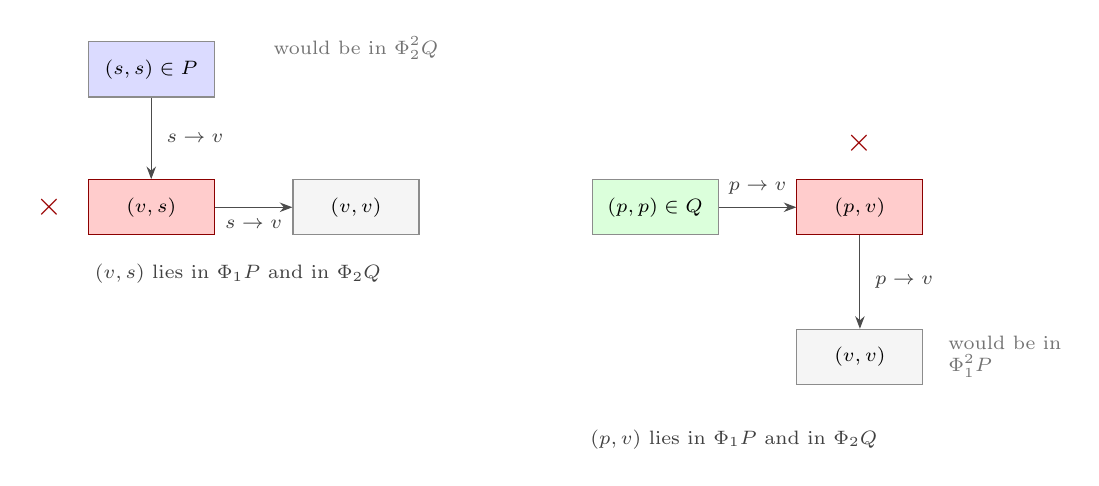
\begin{tikzpicture}[
  cell/.style={draw=black!45,minimum width=1.6cm,minimum height=0.7cm,align=center,
               font=\scriptsize,inner sep=1pt},
  pc/.style={cell,fill=blue!14},
  qc/.style={cell,fill=green!14},
  bad/.style={cell,fill=red!20,draw=red!55!black},
  neut/.style={cell,fill=black!4},
  ar/.style={-{Stealth[length=1.6mm]},draw=black!70},
  lab/.style={font=\scriptsize,text=black!75}
]
% ---- case 1: (v,v) not in Phi_2^2 Q
\node[pc]   (ss) at (0,1.75) {$(s,s)\in P$};
\node[bad]  (vs) at (0,0)    {$(v,s)$};
\node[neut] (vv) at (2.6,0)  {$(v,v)$};
\draw[ar] (ss) -- node[right=2pt,lab] {$s\to v$} (vs);
\draw[ar] (vs) -- node[below=1pt,lab] {$s\to v$} (vv);
\node[font=\large,text=red!60!black,anchor=east] at (-1.0,0) {$\times$};
\node[lab,anchor=north,align=center] at (1.1,-0.6) {$(v,s)$ lies in $\Phi_1P$ and in $\Phi_2Q$};
\node[lab,anchor=south,align=center,text=black!55] at (2.6,1.75) {would be in $\Phi_2^2Q$};
% ---- case 2: (v,v) not in Phi_1^2 P
\node[qc]   (pp) at (6.4,0)     {$(p,p)\in Q$};
\node[bad]  (pv) at (9.0,0)     {$(p,v)$};
\node[neut] (vv2) at (9.0,-1.9) {$(v,v)$};
\draw[ar] (pp) -- node[above=1pt,lab] {$p\to v$} (pv);
\draw[ar] (pv) -- node[right=2pt,lab] {$p\to v$} (vv2);
\node[font=\large,text=red!60!black,anchor=south] at (9.0,0.55) {$\times$};
\node[lab,anchor=north,align=center] at (7.4,-2.7) {$(p,v)$ lies in $\Phi_1P$ and in $\Phi_2Q$};
\node[lab,anchor=west,align=left,text=black!55] at (10.0,-1.9) {would be in\\ $\Phi_1^2P$};
\end{tikzpicture}

\caption{Why the diagonal survives (Step~5 of that proof) and why diagonals never conflict. \emph{Look
 at} the two halves: if a diagonal cell were in $\Phi_2^2Q$ (left) or in $\Phi_1^2P$ (right), the
 cell marked $\times$ would lie in both images at once. \emph{Why it matters:} the pair
 $(\mathcal L,\mathcal R)$ may conflict, but the diagonal members are conflict-free, so the pruning
 lemma is allowed to keep them --- and the diagonal is what makes the pruned pair admissible, i.e.\
 a competitor to $(P,Q)$.}
\label{fig:diagonal}
\end{figure}

\emph{No diagonal member conflicts.} Let $(v,v)\in\Delta$ and $(i,s)\in\mathcal R$ conflict, i.e.\
$v\to i$ and $s\to v$. Then $(s,s)\in P$, and advancing its first coordinate twice along
$s\to v\to i$ puts $(i,s)$ in $\Phi_1^2P$, contradicting $(i,s)\in\mathcal R$. Symmetrically, if
$(p,j)\in\mathcal L$ conflicts with the diagonal member $(v,v)$, then $p\to v$ and $v\to j$, and
advancing the second coordinate of $(p,p)\in Q$ twice along $v\to j$ puts $(p,j)$ in $\Phi_2^2Q$,
contradicting $(p,j)\in\mathcal L$. So every diagonal member is conflict-free, and the preservation
clause of \cref{lem:pruning} applies to all of them.

\steplabel{Step 6: the collisions are uncovered.}
Let $Z,H$ be the sets attached to $\mathcal L,\mathcal R$ by \cref{def:conflict}: a conflict
\[
 (p,j)\in\mathcal L,\qquad (i,s)\in\mathcal R,\qquad p\to i,\qquad s\to j
\]
contributes $(p,s)$ to $H$ and $(i,j)$ to $Z$. We claim
\begin{equation}\label{eq:H-uncovered}
 H\subseteq X^2\setminus\bigl(\Phi_1P\cup\Phi_2Q\bigr),
 \qquad\text{hence}\qquad \abs H\le u .
\end{equation}
Fix such a conflict. If $(p,s)\in\Phi_1P$, then $(u,s)\in P$ for some $u\to p$, and the path
$u\to p\to i$ puts $(i,s)$ in $\Phi_1^2P$, contradicting $(i,s)\in\mathcal R$. If
$(p,s)\in\Phi_2Q$, then $(p,t)\in Q$ for some $t\to s$, and the path $t\to s\to j$ puts $(p,j)$ in
$\Phi_2^2Q$, contradicting $(p,j)\in\mathcal L$. So $(p,s)$ is in neither image, which is
\eqref{eq:H-uncovered}.

\steplabel{Step 7: prune, and contradict maximality.}
Apply \cref{lem:pruning} to $\mathcal L$ and $\mathcal R$. This gives conflict-free
$\mathcal L'\subseteq\mathcal L$ and $\mathcal R'\subseteq\mathcal R$ containing every initially
conflict-free member, so $\Delta\subseteq\mathcal L'\cap\mathcal R'$ by Step~5, and
\begin{equation}\label{eq:prune-cost}
 \abs{\mathcal L\setminus\mathcal L'}+\abs{\mathcal R\setminus\mathcal R'}\le\abs H+q
 \qquad\text{with}\qquad
 q=\abs{\{z\in Z:\ z\text{ covered by no member of }\mathcal L'\cup\mathcal R'\}} .
\end{equation}
Put
\begin{equation}\label{eq:u-prime}
 u'=\abs X^2-\abs{\Phi_1\mathcal L'}-\abs{\Phi_2\mathcal R'} .
\end{equation}
Since $\mathcal L'$ and $\mathcal R'$ have no conflicts, $\Phi_1\mathcal L'\cap\Phi_2\mathcal R'=\varnothing$
(\cref{rem:compat}), so $u'$ is the number of points covered by neither of them. A point is covered
by a kept left member exactly when it lies in $\Phi_1\mathcal L'$, and by a kept right member exactly
when it lies in $\Phi_2\mathcal R'$. Hence the points of $Z$ that are covered by no member of
$\mathcal L'\cup\mathcal R'$ are exactly the points of $Z$ outside $\Phi_1\mathcal L'\cup\Phi_2\mathcal R'$,
of which there are at most $u'$; so $q\le u'$. By \eqref{eq:prune-cost} and \eqref{eq:H-uncovered},
at most $\abs H+q\le u+u'$ members were deleted. Using \eqref{eq:gain},
\begin{align}
 \abs{\mathcal L'}+\abs{\mathcal R'}+u'
 &\ge\abs{\mathcal L}+\abs{\mathcal R}-(u+u')+u'\notag\\
 &=\abs{\mathcal L}+\abs{\mathcal R}-u>M+2u-u=M+u .
 \label{eq:contradiction}
\end{align}
But $(\mathcal L',\mathcal R')$ is an admissible pair: it is compatible and contains the diagonal. So
\eqref{eq:contradiction} contradicts the maximality of $(P,Q)$ in \eqref{eq:objective}. This proves
\cref{prop:no-concavity}.
\end{proof}

\begin{figure}[t]
\centering
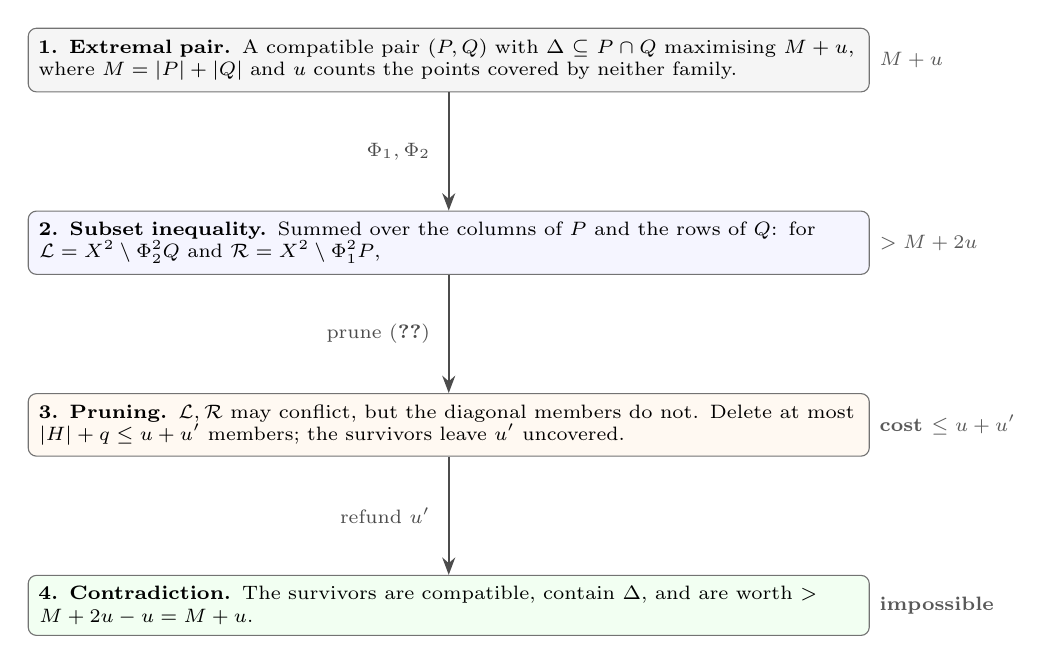
\begin{tikzpicture}[
  stage/.style={draw=black!55,rounded corners=3pt,align=left,font=\scriptsize,
                inner sep=4pt,text width=10.4cm,fill=#1},
  stage/.default=white,
  val/.style={font=\scriptsize\bfseries,text=black!65,anchor=west},
  ar/.style={-{Stealth[length=2.2mm]},draw=black!70,thick},
  lab/.style={font=\scriptsize,text=black!70,align=left}
]
\node[stage=black!4] (s1) at (0,0)
 {\textbf{1. Extremal pair.} A compatible pair $(P,Q)$ with $\Delta\subseteq P\cap Q$ maximising
  $M+u$, where $M=\abs P+\abs Q$ and $u$ counts the points covered by neither family.};
\node[val] at (s1.east) {$M+u$};
\node[stage=blue!4,below=15mm of s1] (s2)
 {\textbf{2. Subset inequality.} Summed over the columns of $P$ and the rows of $Q$: for
  $\mathcal L=X^2\setminus\Phi_2^2Q$ and $\mathcal R=X^2\setminus\Phi_1^2P$,};
\node[val] at (s2.east) {$>M+2u$};
\node[stage=orange!5,below=15mm of s2] (s3)
 {\textbf{3. Pruning.} $\mathcal L,\mathcal R$ may conflict, but the diagonal members do not. Delete
  at most $\abs H+q\le u+u'$ members; the survivors leave $u'$ uncovered.};
\node[val] at (s3.east) {cost $\le u+u'$};
\node[stage=green!5,below=15mm of s3] (s4)
 {\textbf{4. Contradiction.} The survivors are compatible, contain $\Delta$, and are worth
  $>M+2u-u=M+u$.};
\node[val] at (s4.east) {impossible};
\draw[ar] (s1.south) -- node[left=3pt,lab] {$\Phi_1,\Phi_2$} (s2.north);
\draw[ar] (s2.south) -- node[left=3pt,lab] {prune (\cref{lem:pruning})} (s3.north);
\draw[ar] (s3.south) -- node[left=3pt,lab] {refund $u'$} (s4.north);
\end{tikzpicture}

\caption{The four moves of \cref{sec:incompatibility}, with the numbers attached. \emph{Read from
 left to right:} the extremal compatible pair $(P,Q)$ has value $M+u$; the subset inequalities,
 summed over columns and rows, produce the complements with value greater than $M+2u$; the pruning
 lemma deletes at most $u+u'$ members and leaves $u'$ points uncovered; the survivors are compatible,
 contain the diagonal, and have value greater than $M+u$ --- which is impossible. \emph{Why it
 matters:} the figure shows where each of the two copies of $u$ in the gain is spent: one pays for
 the collisions $H$, the other survives as the refunded $u'$.}
\label{fig:extremal}
\end{figure}

\subsection{Hypotheses, weights, and where strictness is needed}\label{sec:remarks4}

\begin{remark}[Where each hypothesis of \cref{prop:no-concavity} is used]\label{rem:hypotheses}
The proof uses exactly three properties of $G$, and it is worth knowing where.
\begin{itemize}[leftmargin=1.4em,itemsep=2pt,topsep=1pt]
\item \emph{The relation is oriented}, in four places: the diagonal is compatible with itself
 (Step~1); the diagonal survives both complement families (Step~5, first half); no diagonal member
 conflicts (Step~5, second half); and $N_2^+(v)=F^2(\{v\})\setminus F(\{v\})$ in the first place.
 All four uses are of the same fact --- there is no pair of opposite arcs --- and each of them would
 fail for a general digraph.
\item \emph{Every vertex has an in-neighbor}, in two places: a column $P_j$ that equals all of $X$
 would put $X\times\{j\}$ inside $\Phi_1P$ and a single in-neighbor of $j$ would then put $(w,j)$
 inside $\Phi_2Q$ (Step~2); and the same for rows. Without in-neighbors, \eqref{eq:hypothesis} cannot
 be applied to the columns and rows at all.
\item \emph{Strict concavity} \eqref{eq:hypothesis}, in one place only: Step~3, summed over the
 columns and the rows. Everything after that is counting.
\end{itemize}
So a reader checking the proof should watch exactly four steps: 1, 2, 3 and 5.
\end{remark}

\begin{remark}[Why the objective weights uncovered points with coefficient exactly $1$]\label{rem:lambda}
Suppose we maximised $\abs P+\abs Q+\lambda u$ for some other $\lambda>0$. The gain of Step~4 is
unchanged, $>M+2u$; the pruning deletes at most $\abs H+q\le u+u'$ members and the survivors have
$u'$ uncovered points, so the new value is larger than
\[
 M+2u-(u+u')+\lambda u'=\underbrace{M+\lambda u}_{\text{old value}}+(1-\lambda)u+(\lambda-1)u'
 =(\text{old value})+(\lambda-1)(u'-u).
\]
This is a strict improvement only if $(\lambda-1)(u'-u)\ge0$. For $\lambda=1$ the last term vanishes
and the strictness comes entirely from the strict gain, which is what we want; for $\lambda<1$ the
argument fails whenever $u'>u$, and for $\lambda>1$ it fails whenever $u'<u$. Since both cases occur,
$\lambda=1$ is the only weight that works for all instances. The coefficient $1$ on $u$ is therefore
forced by the structure of the pruning bound, not chosen for convenience.
\end{remark}

\begin{example}[Where the argument stops on a directed triangle]\label{ex:triangle}
Let $G$ be the directed triangle $a\to b\to c\to a$, which has all indegrees positive, and let
$P=Q=\Delta$. Then
\[
 \abs X^2=9,\qquad M=\abs P+\abs Q=6,\qquad u=9-3-3=3,
\]
because $\Phi_1\Delta=\Phi_2\Delta=\{(i,j):j\to i\}$, the arc set, has three elements, and
and $\Phi_1^2\Delta=\Phi_2^2\Delta=\Delta$, so the two complement families of Step~4 satisfy
\[
 \abs{\mathcal L}+\abs{\mathcal R}=2\cdot9-3-3=12=M+2u .
\]
The gain is $M+2u$ exactly, not more, because strict concavity fails for this graph: at $U=\{a\}$ we
have $1+1=2=2\cdot1$. Consequently the survivors are worth only
$\ge M+2u-(u+u')+u'=M+u$, which does not contradict maximality. \Cref{ex:triangle} therefore shows
precisely which strict inequality the whole argument rests on: the concavity hypothesis must be
strict, and the contradiction is the difference between `>' and `$\ge$'.
\end{example}

\begin{proof}[Proof of \cref{thm:main}]
If \cref{thm:main} were false, \cref{prop:reduction} would produce a nonempty finite oriented graph
with positive indegrees satisfying \eqref{eq:impossible} for every nonempty proper vertex set, and
\cref{prop:no-concavity} says that no such graph exists.
\end{proof}

\begin{checkpoint}
The proof of the main theorem is complete, and it used exactly two ingredients beyond the definitions:
the subset inequality (\cref{lem:deficit,lem:blowup}, giving \cref{prop:reduction}) and the pruning
lemma (\cref{lem:pruning}). Everything in the remaining two sections is a consequence.
\end{checkpoint}

\begin{remark}[Why the argument cannot be short-circuited]\label{rem:why-hard}
It is instructive to see which step fails if one tries to simplify the argument.
\begin{itemize}[leftmargin=1.4em,itemsep=2pt,topsep=1pt]
\item \emph{Why not just take $P=Q=\Delta$ and stop?} The diagonal is admissible --- that is Step~1
  --- but its value is $2\abs X+\abs X^2-2\abs A$ (because $\Phi_1\Delta=\{(i,j):j\to i\}$ and
  $\Phi_2\Delta=\{(i,j):i\to j\}$ are both copies of the arc set $A$), and what is needed is a pair
  that beats \emph{every} admissible pair. The diagonal's role is to make the maximum exist and to
  survive the pruning; the size has to come from the extremal choice.
\item \emph{Why not take larger $P,Q$ greedily?} Compatibility is a global condition: a single added
  member can cover an entire line of cells and destroy compatibility with the other family. The
  extremal choice is what handles this; there is no local augmentation argument.
\item \emph{Why is the pruning step not circular?} The pruning lemma is a statement about arbitrary
  relations; it does not know that $\mathcal L,\mathcal R$ come from an extremal pair. It is applied
  once, and the only thing it needs is that the diagonal members are conflict-free, which is Step~5.
\item \emph{Where does the strictness come from?} From \eqref{eq:hypothesis}, which is strict; the
  gain \eqref{eq:gain} is therefore strict, and the deletion bound is not strict, so the inequality
  survives. If \eqref{eq:hypothesis} were weak, the proof would only give $M+2u\ge\ldots$ and no
  contradiction.
\end{itemize}
\end{remark}

\section{Weighted consequences}\label{sec:weighted}

\begin{contract}
\textbf{Assumes:} \cref{thm:main}. \quad
\textbf{Produces:} the vertex- and arc-weighted forms of the conjecture
(\cref{cor:weighted}). \textbf{Why:} these are the forms in which the conjecture is usually applied;
the passage from the unweighted statement to them is Seacrest's, and is quoted rather than reproved.
Nothing in this section is used in the proof of \cref{thm:main}.
\end{contract}

The weighted forms come in two quantifier orders, and the difference matters. One can ask that
\emph{for every} weighting there be a vertex that does well (a max-min statement), or that there be
\emph{one} weighting for which every vertex does well (a min-max statement). Both hold, and both
follow from \cref{thm:main} through the equivalence proved by Seacrest~\cite{Seacrest2015}.

\begin{corollary}[Weighted second-neighborhood forms]\label{cor:weighted}
Let $D$ be a nonempty finite oriented graph and $A(D)$ its arc set. For a vertex weighting
$\eta:V(D)\to[0,\infty)$ write $\eta(S)=\sum_{x\in S}\eta(x)$. Then:
\begin{enumerate}[label=\textup{(\roman*)},leftmargin=1.6em,itemsep=3pt]
\item for every vertex weighting $\eta:V(D)\to[0,\infty)$ there is a vertex $v$ with
  \[
   \eta(N_1^+(v))\le\eta(N_2^+(v));
  \]
\item there is a vertex weighting $\eta:V(D)\to[0,\infty)$ with $\sum_{x\in V(D)}\eta(x)=1$ such that
  \[
   \eta(N_1^+(v))\le\eta(N_2^+(v))\qquad\text{for every }v\in V(D),
  \]
  whose entries need not all be positive;
\item for every arc weighting $w:A(D)\to[0,\infty)$, extended by $w(vs)=0$ when $vs\notin A(D)$, and
  with
  \[
   \beta_v^w(s)=\max\Bigl(\{0\}\cup\{w(us)-w(vs):\ u\in V(D),\ v\to u\to s\}\Bigr),
  \]
  there is a vertex $v$ with
  \[
   \sum_{s\in V(D)}\beta_v^w(s)\ \ge\ \sum_{u\in N_1^+(v)}w(vu).
  \]
\end{enumerate}
\end{corollary}

\inwords{Weighted by nonnegative numbers, either every weighting admits a good vertex, or one
weighting makes every vertex good; and the same holds for weights on arcs, with a two-step maximum
in place of the second neighborhood.}

\begin{proof}
\emph{(iii)} is Seacrest's arc-weighted conjecture, which his Proposition~2 shows to be equivalent to
the unweighted conjecture~\cite{Seacrest2015}; \cref{thm:main} is the unweighted conjecture, so (iii)
holds.

\emph{(i) follows from (iii).} Given $\eta$, set $w(us)=\eta(s)$ for every arc $us$. Then for
$v,s\in V(D)$,
\[
 \beta_v^w(s)=\begin{cases}\eta(s),&s\in N_2^+(v),\\ 0,&s\notin N_2^+(v),\end{cases}
\]
as \cref{fig:beta} illustrates: if $v\to s$ then every eligible difference
$w(us)-w(vs)=\eta(s)-\eta(s)$ is $0$, and if $s$ is at exact distance two from $v$ then $w(vs)=0$ and
the maximum is $\eta(s)$. So the two sides of (iii) become $\eta(N_2^+(v))$ and $\eta(N_1^+(v))$,
which is (i).

\emph{(ii) follows from (i) by duality.} Let $M_D$ be the matrix with rows and columns indexed by
$V(D)$, with entry $1$ at $(v,s)$ when $s\in N_2^+(v)$, entry $-1$ when $s\in N_1^+(v)$, and entry
$0$ otherwise. Reversing all arcs transposes this matrix, $M_{\overleftarrow D}=M_D^{\mathsf T}$,
because reversing swaps the roles of first and second out-neighborhoods. By Farkas' lemma in the form
used by Seacrest~\cite[Theorem~1]{Seacrest2015}, exactly one of the following holds: there is a
nonzero $\eta\ge0$ with $M_D\eta\ge0$, or there is $\xi\ge0$ with $M_D^{\mathsf T}\xi<0$ entrywise.
The second alternative is impossible: it would say that in the reversed graph $\overleftarrow D$ every
vertex $v$ has $\xi(N_1^+(v))>\xi(N_2^+(v))$, contradicting (i) applied to $\overleftarrow D$ with the
weighting $\xi$. So the first alternative holds; normalizing $\eta$ to total weight $1$ gives (ii).
\end{proof}

\begin{figure}[t]
\centering
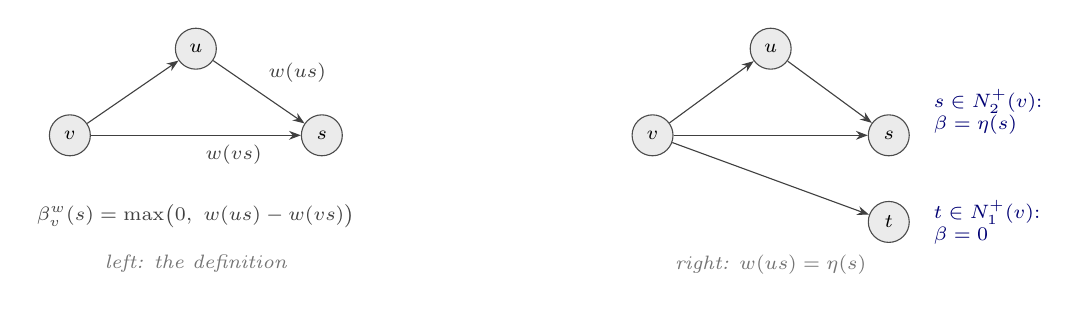
\begin{tikzpicture}[
  v/.style={circle,draw=black!70,fill=black!8,inner sep=0pt,minimum size=5.2mm,font=\scriptsize},
  ar/.style={-{Stealth[length=1.5mm]},draw=black!75},
  lab/.style={font=\scriptsize,text=black!75},
  wl/.style={font=\scriptsize,text=blue!45!black,align=left},
  pan/.style={font=\scriptsize\itshape,text=black!55}
]
% ---------------- left: the definition
\node[v] (v) at (0,1.3) {$v$};
\node[v] (u) at (1.6,2.4) {$u$};
\node[v] (s) at (3.2,1.3) {$s$};
\draw[ar] (v) -- (u);
\draw[ar] (u) -- node[above right=0pt,lab] {$w(us)$} (s);
\draw[ar] (v) -- node[below right=0pt,lab] {$w(vs)$} (s);
\node[lab,anchor=north] at (1.6,0.55) {$\beta_v^w(s)=\max\bigl(0,\ w(us)-w(vs)\bigr)$};
\node[pan,anchor=north] at (1.6,-0.1) {left: the definition};
% ---------------- right: the specialization
\begin{scope}[shift={(7.4,0)}]
\node[v] (v2) at (0,1.3) {$v$};
\node[v] (u2) at (1.5,2.4) {$u$};
\node[v] (s3) at (3.0,1.3) {$s$};
\node[v] (t2) at (3.0,0.2) {$t$};
\draw[ar] (v2) -- (u2);
\draw[ar] (u2) -- (s3);
\draw[ar] (v2) -- (s3);
\draw[ar] (v2) -- (t2);
\node[wl,anchor=west] at (3.45,1.6) {$s\in N_2^+(v)$:\\ $\beta=\eta(s)$};
\node[wl,anchor=west] at (3.45,0.2) {$t\in N_1^+(v)$:\\ $\beta=0$};
\node[pan,anchor=north] at (1.5,-0.1) {right: $w(us)=\eta(s)$};
\end{scope}
\end{tikzpicture}

\caption{The arc weighting $\beta_v^w$ of \cref{cor:weighted}(iii), and the substitution of (i).
\emph{Left:} for each two-step path $v\to u\to s$ one compares the last arc weight $w(us)$ with the
first arc weight $w(vs)$; $\beta_v^w(s)$ is the largest excess over all intermediate vertices $u$,
and $0$ if there is none. \emph{Right:} with the constant weighting $w(us)=\eta(s)$ the excess is
$\eta(s)$ at an exact second out-neighbor and $0$ everywhere else, so the inequality of (iii) becomes
$\eta(N_2^+(v))\ge\eta(N_1^+(v))$. \emph{Why it matters:} the figure shows why the arc-weighted form
is the right common generalization: its two sides are a sum over out-arcs and a sum over two-step
excesses, and the vertex-weighted statements are the two specializations.}
\label{fig:beta}
\end{figure}

\begin{remark}[What is new here and what is quoted]\label{rem:quoted}
Only \cref{thm:main} is new. The passage from it to \cref{cor:weighted} is Seacrest's: (iii)
$\Leftrightarrow$ unweighted is his Proposition~2, and the Farkas duality between (i) and (ii) is his
Theorem~1. We quote these rather than reprove them, and we have verified that the statements quoted
are the ones used: in particular, (iii) is the form with a \emph{maximum over intermediate vertices},
not a sum over paths, and the arc weights are allowed to vanish.
\end{remark}

\section{Directed-cycle consequences}\label{sec:cycles}

\begin{contract}
\textbf{Assumes:} \cref{thm:main}. \quad
\textbf{Produces:} degree and order bounds for oriented graphs without a directed triangle, including
a minimum-degree threshold of $n/3$ for the existence of a directed triangle
(\cref{cor:cycles}). \textbf{Why:} these are the standard corollaries; they show what the theorem buys
and they are the reason the conjecture is studied alongside the Caccetta--H\"aggkvist problem.
Nothing here is used earlier.
\end{contract}

The mechanism is one observation: in an oriented graph without a directed triangle, no second
out-neighbor can be an in-neighbor, because a path $v\to u\to w$ together with the arc $w\to v$ would
be a directed triangle. So the second out-neighborhood sits inside the set of \emph{non-neighbors},
and \cref{thm:main} becomes a counting statement about three disjoint classes of vertices.

\begin{corollary}[Non-neighbors and directed cycles]\label{cor:cycles}
Let $D$ be a nonempty finite oriented graph of order $n$. For $v\in V(D)$ put
\[
 N_1^-(v)=\{u:u\to v\},\qquad d^\pm(v)=\abs{N_1^\pm(v)},\qquad
 \delta^\pm(D)=\min_{x\in V(D)}d^\pm(x),
\]
and let
\[
 \overline N(v)=V(D)\setminus\bigl(\{v\}\cup N_1^+(v)\cup N_1^-(v)\bigr)
\]
be the set of \emph{non-neighbors} of $v$ (vertices adjacent to $v$ in neither direction). Then:
\begin{enumerate}[label=\textup{(\roman*)},leftmargin=1.6em,itemsep=3pt]
\item if $D$ has no directed $3$-cycle, then some vertex $v$ satisfies
  \[
   d^+(v)\le\abs{\overline N(v)},\qquad n-1\ge2d^+(v)+d^-(v);
  \]
\item if $\delta^+(D)\ge n/3$ and $\delta^-(D)\ge n/3$, then $D$ contains a directed $3$-cycle;
\item if $r\ge1$ is an integer, $d^+(v)=d^-(v)=r$ for every vertex, and $D$ has directed girth
  exactly four, then $n\ge3r+1$.
\end{enumerate}
Here the directed girth is the length of a shortest directed cycle.
\end{corollary}

\inwords{Without a directed triangle, some vertex has at most as many out-neighbors as non-neighbors,
which forces $n-1\ge2d^++d^-$; hence minimum in- and out-degree at least $n/3$ forces a directed
triangle, and a regular oriented graph of girth four satisfies $n\ge3r+1$.}

\usedin{Not used in the proof of \cref{thm:main}; these are consequences, and \cref{sec:history}
records where they appear in the literature.}

\begin{proof}
Assume that $D$ has no directed $3$-cycle, and let $w\in N_2^+(v)$; choose a path $v\to u\to w$. By
the definition of exact distance, $w\ne v$ and $w\notin N_1^+(v)$. If also $w\in N_1^-(v)$, then
$w\to v$, and $v\to u\to w\to v$ is a directed $3$-cycle --- impossible. Hence
\begin{equation}\label{eq:N2-in-Z}
 N_2^+(v)\subseteq\overline N(v)\qquad\text{for every }v .
\end{equation}
By \cref{thm:main} there is a vertex $v$ with
\[
 d^+(v)=\abs{N_1^+(v)}\le\abs{N_2^+(v)}\overset{\eqref{eq:N2-in-Z}}{\le}\abs{\overline N(v)} .
\]
Since $D$ is oriented, $N_1^+(v)$ and $N_1^-(v)$ are disjoint and both avoid $v$, so the three sets in
the definition of $\overline N(v)$ partition $V(D)\setminus\{v\}$:
\begin{equation}\label{eq:partition}
 n-1=d^+(v)+d^-(v)+\abs{\overline N(v)}\ge 2d^+(v)+d^-(v),
\end{equation}
which is (i); \cref{fig:cycles} draws the partition.

For (ii), if $D$ had no directed $3$-cycle then (i) would give
\[
 n-1\ge2\delta^+(D)+\delta^-(D)\ge2\cdot\frac n3+\frac n3=n,
\]
a contradiction. (The degrees are integers, so $\delta^\pm(D)\ge n/3$ means
$\delta^\pm(D)\ge\lceil n/3\rceil$; the argument covers the endpoint when $3$ divides $n$.)

For (iii), directed girth four excludes directed triangles, and $d^+=d^-=r$ turns
\eqref{eq:partition} into $n-1\ge3r$.
\end{proof}

\begin{figure}[t]
\centering
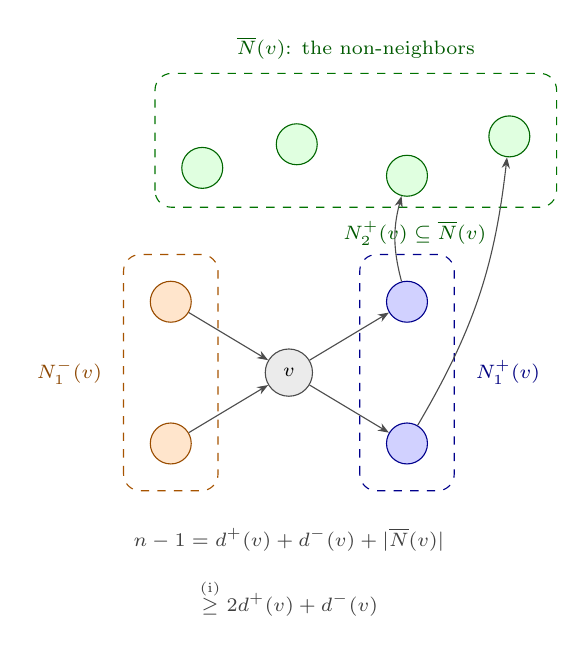
\begin{tikzpicture}[
  v/.style={circle,draw=black!70,fill=black!8,inner sep=0pt,minimum size=6mm,font=\scriptsize},
  o/.style={circle,draw=blue!55!black,fill=blue!18,inner sep=0pt,minimum size=5.2mm,font=\scriptsize},
  i/.style={circle,draw=orange!60!black,fill=orange!20,inner sep=0pt,minimum size=5.2mm,font=\scriptsize},
  nn/.style={circle,draw=green!40!black,fill=green!12,inner sep=0pt,minimum size=5.2mm,font=\scriptsize},
  ar/.style={-{Stealth[length=1.4mm]},draw=black!70},
  lab/.style={font=\scriptsize,text=black!75}
]
% regions
\draw[green!45!black,dashed,rounded corners=6pt] (-1.7,2.1) rectangle (3.4,3.8);
\draw[orange!65!black,dashed,rounded corners=6pt] (-2.1,-1.5) rectangle (-0.9,1.5);
\draw[blue!55!black,dashed,rounded corners=6pt] (0.9,-1.5) rectangle (2.1,1.5);
% vertices
\node[v] (v) at (0,0) {$v$};
\node[o] (a) at (1.5,0.9) {};
\node[o] (b) at (1.5,-0.9) {};
\node[i] (c) at (-1.5,0.9) {};
\node[i] (d) at (-1.5,-0.9) {};
\node[nn] (e) at (0.1,2.9) {};
\node[nn] (f) at (1.5,2.5) {};
\node[nn] (g) at (2.8,3.0) {};
\node[nn] (h) at (-1.1,2.6) {};
% arcs
\draw[ar] (v) -- (a);
\draw[ar] (v) -- (b);
\draw[ar] (c) -- (v);
\draw[ar] (d) -- (v);
\draw[ar] (a) to[bend left=15] (f);
\draw[ar] (b) to[bend right=12] (g);
% labels
\node[lab,anchor=west,text=blue!50!black] at (2.25,0) {$N_1^+(v)$};
\node[lab,anchor=east,text=orange!55!black] at (-2.25,0) {$N_1^-(v)$};
\node[lab,anchor=south,text=green!35!black] at (0.85,3.85) {$\overline N(v)$: the non-neighbors};
\node[lab,anchor=north,text=green!35!black] at (1.6,2.05) {$N_2^+(v)\subseteq\overline N(v)$};
% the count
\node[lab,anchor=north] at (0,-1.85) {$n-1=d^+(v)+d^-(v)+\abs{\overline N(v)}$};
\node[lab,anchor=north] at (0,-2.5) {$\overset{\text{(i)}}{\ge}2d^+(v)+d^-(v)$};
\end{tikzpicture}

\caption{The partition behind \eqref{eq:partition}, in an oriented graph without a directed triangle.
\emph{Look at} the three classes around $v$: out-neighbors, in-neighbors and non-neighbors. The
label inside the third class records \eqref{eq:N2-in-Z}, that the second out-neighborhood
sits inside it: a second out-neighbor that was also an in-neighbor would close a directed
triangle. \emph{Why it matters:} \cref{thm:main} bounds the first class by the second
out-neighborhood, hence by the third class, and the three classes partition $V\setminus\{v\}$; this
gives $n-1\ge2d^++d^-$ with no further input.}
\label{fig:cycles}
\end{figure}

\begin{remark}[Where these statements come from]\label{rem:cycles-history}
Part (i) is the oriented-graph form of Thomass\'e's non-neighbor statement, recorded as
Conjecture~6.12 in Sullivan's survey~\cite{Sullivan2006}; the consequence for minimum in- and
out-degree is noted in Section~3 of the same survey, and the regular girth-four bound in Section~4,
where it is attributed to the Behzad--Chartrand--Wall minimum-order
conjecture~\cite{BehzadChartrandWall1970}. The point of recording them here is that they follow from
\cref{thm:main} alone, with no additional hypothesis on $D$.
\end{remark}

\appendix
\section{Toolkit: the five facts we use from outside graph theory}\label{app:toolkit}

Everything in this appendix is standard, and none of it is new. It is collected here, with proofs,
because the rewrite is addressed to a reader who has had one course in graph theory and none in
linear algebra beyond the rank of a matrix. The main text uses \cref{thm:konig,lem:minor-matching}
repeatedly; \cref{thm:farkas} is used exactly once, in \cref{sec:weighted}, and a reader willing to
take the vertex-weighted corollary on trust may skip it.

\subsection{Matchings, covers, and K\H{o}nig's theorem}\label{app:konig}

Let $\Gamma$ be a bipartite graph with parts $A$ and $B$. A \emph{matching} is a set of edges no two
of which share a vertex; $\nu(\Gamma)$ is the largest size of a matching. A \emph{vertex cover} is a
set $K\subseteq A\cup B$ meeting every edge.

\begin{theorem}[K\H{o}nig]\label{thm:konig}
In a bipartite graph $\Gamma$, the maximum size of a matching equals the minimum size of a vertex
cover. Moreover, if $\mathcal M$ is a maximum matching and $A_0$ is the set of vertices of $A$
unmatched by $\mathcal M$, then the set $K$ constructed below is a vertex cover with
$\abs K=\abs{\mathcal M}$ that contains exactly one endpoint of every edge of $\mathcal M$ and no
unmatched vertex.
\end{theorem}

\begin{proof}
A cover has at least one vertex from each edge of a matching, so $\abs K\ge\nu(\Gamma)$ for every
cover $K$; it suffices to exhibit a cover of size $\nu(\Gamma)$. Let $\mathcal M$ be a maximum
matching. Starting from all unmatched vertices of $A$, follow edges \emph{outside} $\mathcal M$ from
$A$ to $B$ and edges \emph{in} $\mathcal M$ from $B$ to $A$; let $W_A\subseteq A$ and $W_B\subseteq B$
be the sets of vertices reached.

\emph{No unmatched vertex of $B$ is reached}: an alternating path from an unmatched vertex of $A$ to
an unmatched vertex of $B$ would be augmenting, and augmenting it would enlarge $\mathcal M$.

\emph{The endpoints of a matched edge are either both reached or both unreached}. If the $B$-endpoint
is reached, the matching edge leads to its $A$-endpoint, so that is reached too; conversely a reached
$A$-vertex that is matched was reached along its matching edge from its partner.

Put $K=(A\setminus W_A)\cup W_B$. It covers every edge: an edge $ab$ with $a\in W_A$ and
$b\notin W_B$ would be neither outside $\mathcal M$ (then $b$ would be reached) nor in $\mathcal M$
(since matched endpoints share their status). It contains exactly one endpoint of each matched edge
and no unmatched vertex, because every unmatched vertex of $A$ lies in $W_A$ and, by the first
paragraph, no unmatched vertex of $B$ lies in $W_B$. Hence
$\abs K=\abs{\mathcal M}=\nu(\Gamma)$.
\end{proof}

\subsection{Ranks}\label{app:ranks}

For a real matrix $M$ with $c$ columns, \emph{rank--nullity} is the statement
$\dim\ker M=c-\rank M$: the rank is the dimension of the image and the domain splits as the kernel
direct sum a complement.

\begin{lemma}[Sylvester's rank inequality]\label{lem:sylvester}
For real matrices $X$ (with $c$ columns) and $Y$ (with $c$ rows),
\[
 \rank(XY)\ \ge\ \rank X-\dim\ker Y .
\]
\end{lemma}

\begin{proof}
The map $Y$ sends $\im X$ onto $\im(XY)$, and its kernel on $\im X$ is $\im X\cap\ker Y$. A linear
map on a space of dimension $d$ with kernel of dimension $e$ has image of dimension $d-e$, so
$\rank(XY)=\dim\im X-\dim(\im X\cap\ker Y)\ge\rank X-\dim\ker Y$.
\end{proof}

\begin{lemma}[A nonzero minor exhibits a matching]\label{lem:minor-matching}
Let $T\subseteq I\times J$ be finite and let $M$ be a real matrix supported on $T$, that is, with
$M_{ij}=0$ whenever $(i,j)\notin T$. Then
\[
 \rank M\ \le\ \nu(T),
\]
where $\nu(T)$ is the largest size of a set of entries of $T$ no two in the same row or column.
In particular, if $\mathcal M$ is a maximum matching in the support $T$, then every matrix supported
on $T$ has rank at most $\abs{\mathcal M}$, and equality is attained by some matrix supported
on $T$.
\end{lemma}

\begin{proof}
Let $r=\rank M$, so $M$ has an $r\times r$ submatrix $\widehat M$ with $\det\widehat M\ne0$. Expanding
the determinant,
\[
 \det\widehat M=\sum_{\sigma}\operatorname{sgn}(\sigma)\prod_{i}\widehat M_{i\sigma(i)},
\]
and every product in the sum is a product of entries of $T$ with distinct rows and distinct columns,
i.e.\ of a matching of size $r$ in $T$; such a matching exists as soon as one product is nonzero, and
one is nonzero because the sum is. Hence $r\le\nu(T)$.

For the last sentence: the identity matrix on a matching of size $\nu(T)$ (entries $1$ on the matched
pairs, $0$ elsewhere) is supported on $T$ and has rank $\nu(T)$.
\end{proof}

\begin{remark}[What we do and do not need]\label{rem:no-edmonds}
The classical statement is that the \emph{maximum rank} over matrices supported on $T$ equals
$\nu(T)$; the second half of \cref{lem:minor-matching} is that statement, in the easy direction,
and we use only this. In the proof of the matching bound (\cref{sec:matching}) the two inequalities
are used as follows: an upper bound $\rank L\le\ell$ for \emph{every} assignment of the variables,
because the support of $L$ contains no matching larger than $\ell$ (\cref{lem:minor-matching},
first part); and the existence of \emph{one} assignment with $\rank L=\ell$, exhibited by an explicit
minor whose determinant is a nonzero polynomial (\cref{sec:matching}, Step~5). No appeal to the
hard direction is needed, and in particular this document does not rely on the
Edmonds/Egerv\'ary rank formula.
\end{remark}

\subsection{The Farkas alternative}\label{app:farkas}

\begin{theorem}[Farkas, in the form we use]\label{thm:farkas}
For a real matrix $M$ with $n$ columns, exactly one of the following holds:
\begin{enumerate}[label=\textup{(\roman*)},leftmargin=1.6em,itemsep=1pt,topsep=1pt]
\item there is $\eta\in\R^n$ with $\eta\ge0$, $\eta\ne0$ and $M\eta\ge0$;
\item there is $\xi\ge0$ with $M^{\mathsf T}\xi<0$ in every coordinate.
\end{enumerate}
\end{theorem}

\begin{proof}[Sketch]
Apply Farkas' lemma in the form: exactly one of
$\{\xi\ge0:\ A\xi\ge b\}\ne\varnothing$ and $\{\eta\ge0:\ A^{\mathsf T}\eta\le0,\ b^{\mathsf T}\eta>0\}\ne\varnothing$
holds. Take $A=-M^{\mathsf T}$ and $b=\mathbf 1$. The first alternative becomes
$\xi\ge0$, $M^{\mathsf T}\xi\le-\mathbf 1$, which is equivalent to (ii) by rescaling; the second
becomes $\eta\ge0$, $M\eta\ge0$, $\mathbf 1^{\mathsf T}\eta>0$, which is (i).
\end{proof}

\begin{remark}[Where each external input is used]\label{rem:inputs}
For the main theorem, the only inputs from outside the definitions are \cref{thm:konig} and
\cref{lem:sylvester,lem:minor-matching} (all proved above, all elementary). The weighted forms of
\cref{sec:weighted} additionally use \cref{thm:farkas} for part (ii) and Seacrest's
equivalence~\cite{Seacrest2015} for part (iii); \cref{sec:cycles} uses nothing beyond
\cref{thm:main}.
\end{remark}

\appendix
\section{Proof dependency graph}\label{app:depgraph}

\begin{figure}[h]
\centering
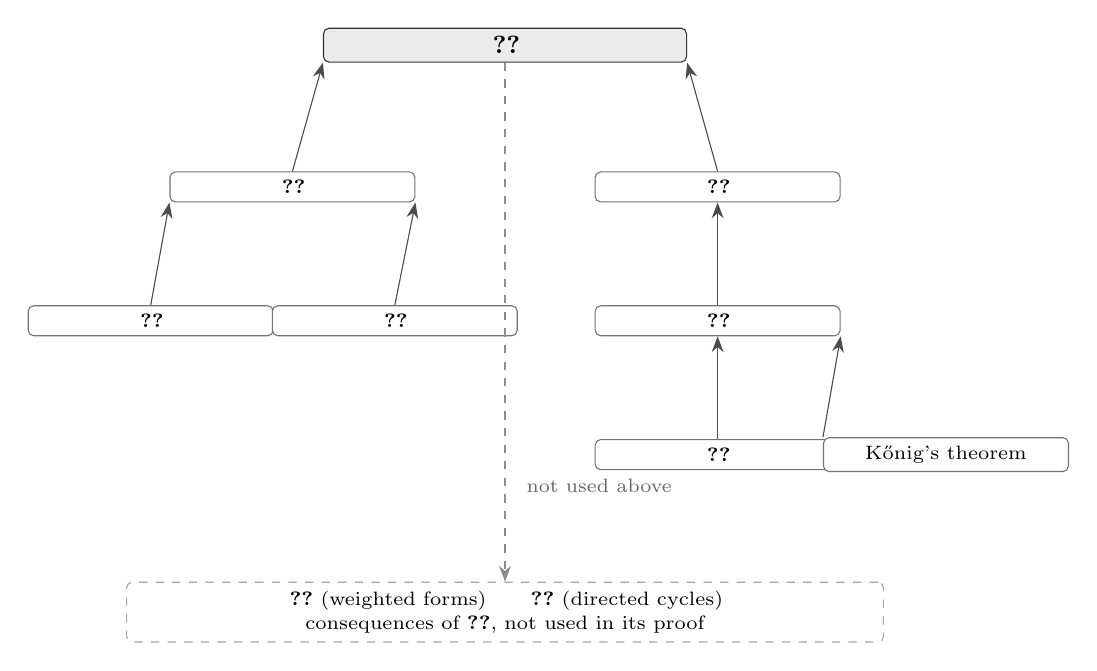
\begin{tikzpicture}[
  st/.style={draw=black!55,rounded corners=2pt,align=center,font=\scriptsize,inner sep=3pt,
             text width=2.9cm,fill=white},
  thm/.style={st,draw=black!80,fill=black!8,font=\small,text width=4.4cm},
  dep/.style={-{Stealth[length=2mm]},draw=black!70},
  ddep/.style={-{Stealth[length=2mm]},draw=black!45,dashed},
  cons/.style={st,draw=black!35,dashed,text width=9.4cm},
  lab/.style={font=\scriptsize,text=black!60}
]
\node[thm] (T) at (0,0) {\cref{thm:main}};
\node[st] (P2) at (-2.7,-1.8) {\cref{prop:reduction}};
\node[st] (P4) at (2.7,-1.8) {\cref{prop:no-concavity}};
\node[st] (L22) at (-4.5,-3.5) {\cref{lem:deficit}};
\node[st] (L23) at (-1.4,-3.5) {\cref{lem:blowup}};
\node[st] (L31) at (2.7,-3.5) {\cref{lem:pruning}};
\node[st] (L32) at (2.7,-5.2) {\cref{lem:kernel}};
\node[st] (KON) at (5.6,-5.2) {K\H{o}nig's theorem};
\node[cons] (C) at (0,-7.2)
  {\cref{cor:weighted} (weighted forms)\qquad \cref{cor:cycles} (directed cycles)\\[1pt]
   consequences of \cref{thm:main}, not used in its proof};
\draw[dep] (L22.north) -- (P2.south west);
\draw[dep] (L23.north) -- (P2.south east);
\draw[dep] (L31.north) -- (P4.south);
\draw[dep] (L32.north) -- (L31.south);
\draw[dep] (KON.north west) -- (L31.south east);
\draw[dep] (P2.north) -- (T.south west);
\draw[dep] (P4.north) -- (T.south east);
\draw[ddep] (T.south) -- (C.north);
\node[lab,anchor=west] at (0.15,-5.6) {not used above};
\end{tikzpicture}

\caption{Which numbered statement uses which. Read upwards: an arrow from $A$ to $B$ means that the
 proof of $B$ uses $A$. \emph{Look at} the two chains: the theorem uses exactly two propositions, and
 each proposition uses one substantial lemma. \emph{Why it matters:} the dashed box at the bottom shows
 that \cref{cor:weighted,cor:cycles} consume the theorem and feed nothing, so they can be skipped; and
 the two columns are independent of each other, so the reduction and the pruning can be read in
 either order.}
\label{fig:depgraph}
\end{figure}

\begin{table}[h]
\centering
\small
\renewcommand{\arraystretch}{1.2}
\begin{tabular}{@{}llp{6.6cm}@{}}
\toprule
statement & depends on & role \\
\midrule
\cref{thm:main} & \cref{prop:reduction,prop:no-concavity} & main result \\
\cref{prop:reduction} & \cref{lem:deficit,lem:blowup} & counterexample $\Rightarrow$ strict subset inequality \\
\cref{lem:deficit} & minimality of the counterexample & subset deficit in a minimal counterexample \\
\cref{lem:blowup} & \cref{lem:deficit} & amplifies the deficit by the block size \\
\cref{prop:no-concavity} & \cref{lem:pruning} & extremal argument, disjoint from \cref{prop:reduction} \\
\cref{lem:pruning} & \cref{lem:kernel}, K\H{o}nig's theorem & pruning of two families of pairs \\
\cref{lem:kernel} & --- & linear algebra of maximum-rank matrices \\
\cref{cor:weighted} & \cref{thm:main}, \cite{Seacrest2015} & weighted forms (quoted equivalence) \\
\cref{cor:cycles} & \cref{thm:main} & directed-cycle and degree consequences \\
\bottomrule
\end{tabular}
\caption{The same information as \cref{fig:depgraph}, in words.}
\label{tab:dep}
\end{table}

\section{Dictionary: notation and numbering against the original}\label{app:dictionary}

This document follows the original preprint statement by statement, but some symbols were renamed so
that no symbol carries two meanings. The table translates. The numbering of the propositions,
theorems and corollaries agrees with the original; inside the sections it does not, because remarks
are numbered in the same sequence here. The differences are: the original's Lemma~2.3 (blowup) is
this document's Lemma~\ref{lem:blowup}, the original's Lemma~3.1 (pruning) is
Lemma~\ref{lem:pruning}, and the original's Lemma~3.2 (kernels) is Lemma~\ref{lem:kernel}.

{\small
\renewcommand{\arraystretch}{1.15}
\begin{center}
\begin{tabular}{@{}llp{6.2cm}@{}}
\toprule
original & here & why the change \\
\midrule
$F,\ F_D$, $F^2$ & $F$, $F^2$ & unchanged: the vertex-set image operator \\
$F_1,\ F_2$ & $\Phi_1,\ \Phi_2$ & distinct glyphs; $F$ now has one meaning \\
$f$ (inside a block) & $\tau$ & avoids the $F/f$ collision \\
$T\subseteq E$ & $Y\subseteq E$ & $T$ is reserved for the tournament $T_m$ \\
$D_T$ & $D_Y$ & same reason \\
$Q=F(\{v\})\cap(E\setminus T)$ & $Q_v$ & subscripted: $Q$ alone is a family of pairs in \cref{sec:incompatibility} \\
$C=F(Q)\setminus(I\cup T\cup Q\cup F(T))$ & $\Lambda$ & $C$ alone is the right family in \cref{lem:pruning} \\
$d_1,\ d_2$ & $d_1,\ d_2$ & unchanged (degrees at a vertex) \\
$d$ (uncovered), $d'$ & $u$, $u'$ & $d$ is now only a degree \\
$g(T)$ & $g(Y)$ & notation only \\
$H_0=F(S)\cup F^2(S)$ & $W$ & $H$ is the collision set in \cref{lem:pruning} \\
$R,\ C$ (families) & $\mathcal L,\ \mathcal R$ & ``left'' and ``right'' is what they are \\
$R,\ C$ (complements in \S4) & $\mathcal L,\ \mathcal R$ & the same role after pruning \\
$P',\ Q'$ & $\mathcal L',\ \mathcal R'$ & primes never attach to the extremal pair \\
$Z,\ H$ & $Z,\ H$ & unchanged: conflict points, collisions \\
$Z(v)$ (non-neighbors, \S6) & $\overline N(v)$ & $Z$ is taken by the conflict points \\
$u^r,\ v^c$ (lifts) & $\lambda^r,\ \kappa^c$ & $u$ is the uncovered count in \S4 \\
$\lambda^r_a,\ \mu^c_b$ (coefficients) & $\xi^r_a,\ \eta^c_b$ & frees $\lambda$ for the lift vector \\
$k,\ \ell,\ t$ & $k,\ \ell,\ t$ & unchanged \\
$M$ (maximum matching) & $\mathcal M$ & $M=\abs P+\abs Q$ in \S4 \\
\bottomrule
\end{tabular}
\end{center}}

\section{Verification notes}\label{app:checks}

This section records what was checked and how, so that a reader can decide what to trust and what to
re-check. Three kinds of check were used.

\paragraph{(V1) Re-derivation.} Every display of the original was re-derived from the definitions
during the rewrite, and every inequality direction was checked at the point of use. Three places
deserve a note because they are easy to misread.
\begin{itemize}[leftmargin=1.4em,itemsep=2pt,topsep=2pt]
\item In the ledger step of \cref{lem:deficit} the second out-neighborhood of $v$ is confined to $I\cup Y\cup F(Y)$
 \emph{after} the deletion, and this uses $v\in S$ (which comes from the choice of $v$, not from the
 definition of $Q_v$). Without $v\in S$ the inclusion fails.
\item In the block accounting in \cref{lem:blowup} the sum over $S\setminus W$ is extended to $S\setminus F(S)$; this is an
 inequality, not an identity, because a block in $F(S)$ is already fully counted. Treating it as an
 identity would be a mistake.
\item In the kernel step of \cref{lem:pruning} the auxiliary matrix $D^{p,i}$ has maximum rank on $T^{p,i}$, and the
 hypothesis $(s,j)\in T^{p,i}$ is exactly $s\to j$; the vanishing is asserted only for such pairs.
 For $(s,j)\notin T^{p,i}$ the entry $b_{sj}$ is zero and there is nothing to prove.
\end{itemize}

\paragraph{(V2) Exhaustive and random computation.} The combinatorial statements of the paper were
checked on small instances by the scripts in \code{checks/verify.py} of the repository. All checks
pass. The checks are implications and identities rather than the statements themselves, since the
hypotheses of \cref{lem:deficit,lem:blowup,prop:no-concavity} are (conjecturally) unsatisfiable ---
that is the theorem.
\begin{center}
\small
\renewcommand{\arraystretch}{1.15}
\begin{tabular}{@{}p{8.5cm}p{5.6cm}@{}}
\toprule
what & result \\
\midrule
\cref{thm:main} on all oriented graphs with $n\le4$ (760 graphs) and $20000$ random graphs with $5\le n\le9$
 & holds in every case \\
the ledger of the ledger step of \cref{lem:deficit}: the four inclusions, \eqref{eq:g-diff}, the sandwich, and the strict increment
 & $2336$ random $(D,S,Y)$ configurations, no failure \\
the algebra of \cref{lem:blowup}: \eqref{eq:FG}, \eqref{eq:FG2}, \eqref{eq:blowup-main}
 & $24942$ random $(D,m,U)$ instances, no failure \\
the identities of \cref{prop:no-concavity}: fibrewise images, complement gain, diagonal survival, $H$ uncovered
 & $250$ random compatible pairs, no failure \\
the statement of \cref{lem:pruning}, by brute force over all subfamilies
 & $1200$ random instances with $\abs X\le4$, no counterexample \\
\cref{cor:cycles}(i) and the partition \eqref{eq:partition} on $3$-cycle-free graphs; (ii) on random graphs; (iii) on regular girth-$4$ graphs
 & $34114$ graphs, no failure \\
\bottomrule
\end{tabular}
\end{center}

\paragraph{(V3) Formalisation.} A Lean~4 development accompanies this document (\code{lean/} in the
repository). It contains the definitions of oriented graph, first and second out-neighborhood, the
statements of \cref{thm:main,prop:reduction,prop:no-concavity,lem:pruning}, a fully checked proof of
the final assembly of \cref{thm:main} from the two propositions, and a fully checked proof of
\cref{cor:cycles} from \cref{thm:main}. The deep lemmas (\cref{lem:deficit,lem:blowup,lem:pruning})
are stated in Lean but their proofs are not formalised; they are recorded as explicit hypotheses so
that the reader can see exactly which part of the argument is machine-checked and which is not. The
formalisation therefore checks the \emph{statements} and the \emph{logical architecture}, not the
three engines.

\paragraph{What this does not establish.} A pleasant presentation and a passing test suite do not
prove a theorem. The only complete proof in this document is the mathematical text itself; the
computations of (V2) test small cases, and the formalisation of (V3) checks the statements and the
architecture. Neither substitutes for reading the proofs of \cref{lem:deficit,lem:blowup,lem:pruning}.

\section{Index of statements and figures}\label{app:index}

{\small
\renewcommand{\arraystretch}{1.12}
\begin{center}
\begin{tabular}{@{}llp{7.6cm}@{}}
\toprule
\cref{thm:main} & main theorem & every nonempty finite oriented graph has $v$ with $\abs{N_1^+(v)}\le\abs{N_2^+(v)}$ \\
\cref{prop:reduction} & reduction & a counterexample yields \eqref{eq:strict-growth} with positive indegrees \\
\cref{lem:deficit} & subset deficit & $\abs{F^2(S)\setminus F(S)}<\abs{F(S)\setminus S}$ in a minimal counterexample \\
\cref{lem:blowup} & blowup & transitive-tournament blowup gives \eqref{eq:strict-growth} \\
\cref{def:conflict} & conflicts & conflict, conflict point, collision, covering, compatible \\
\cref{lem:pruning} & pruning & compatible subfamilies losing at most $\abs H+q$ members \\
\cref{lem:kernel} & rank lemma & kernels at maximum support rank have disjoint supports \\
\cref{prop:no-concavity} & no graph & \eqref{eq:impossible} is impossible \\
\cref{cor:weighted} & weighted forms & vertex- and arc-weighted statements \\
\cref{cor:cycles} & directed cycles & degree and order bounds without directed triangles \\
\bottomrule
\end{tabular}
\end{center}}

\begin{center}
\small
\renewcommand{\arraystretch}{1.1}
\begin{tabular}{@{}ll@{}}
\cref{fig:definitions}: the two neighborhoods & \cref{fig:roadmap}: architecture of the proof \\
\cref{fig:deficit}: the split of $F(S)$ & \cref{fig:deletion}: the deletion step \\
\cref{fig:blowup}: the blowup & \cref{fig:conflict}: a conflict as a rectangle \\
\cref{fig:pruning-graph}: the augmented graph & \cref{fig:cover}: the charge to the cover \\
\cref{fig:fourmaps}: the commutative square & \cref{fig:grid}: families in the grid \\
\cref{fig:diagonal}: the diagonal survives & \cref{fig:extremal}: the four moves of \cref{sec:incompatibility} \\
\cref{fig:beta}: the arc weighting & \cref{fig:cycles}: non-neighbors and the partition \\
\cref{fig:depgraph}: dependencies & \\
\end{tabular}
\end{center}


\bibliographystyle{plain}
\bibliography{references}
\end{document}
